\documentclass[12pt, a4paper]{article}

% ── Packages ──────────────────────────────────────────────────────────────────
\usepackage[a4paper, top=2.5cm, bottom=2.5cm, left=3.0cm, right=2.5cm, headheight=24.02pt]{geometry}
\usepackage[T1]{fontenc}
\usepackage[utf8]{inputenc}
\usepackage{mathptmx}          % Times New Roman font
\usepackage{amsmath}
\usepackage{amssymb}
\usepackage{pifont}
\usepackage{graphicx}
\usepackage{booktabs}
\usepackage{tabularx}
\usepackage{longtable}
\usepackage{array}
\usepackage{hyperref}
\usepackage{xcolor}
\usepackage{titlesec}

\usepackage{enumitem}
\usepackage{fancyhdr}
\usepackage{caption}
\usepackage{subcaption}
\usepackage{float}
\usepackage{setspace}
\usepackage{tikz}
\usetikzlibrary{positioning,shapes.geometric,shapes.misc,arrows.meta,calc,fit}
\usepackage{mdframed}
\usepackage{tcolorbox}
\tcbuselibrary{skins, breakable}
\usepackage{colortbl}
\usepackage{acronym}           % For list of abbreviations
% References handled manually (IEEE-style numbered list in References section)
% Note: to cite inside text use \cite{} once you add a bibliography, or use [1], [2] notation manually

% ── Table formatting macros ───────────────────────────────────────────────────
\definecolor{tableheader}{RGB}{210, 225, 245}
\definecolor{tablerowalt}{RGB}{240, 244, 248}
\newcommand{\cellHigh}{\cellcolor{unigreen!25}}
\newcommand{\cellMed}{\cellcolor{accentgold!25}}
\newcommand{\cellLow}{\cellcolor{red!15}}
\newcommand{\theadrow}{\rowcolor{tableheader}}
\newcommand{\rowalt}{\rowcolor{tablerowalt}}
\newcommand{\crossmark}{\ding{55}}

% ── Colors ────────────────────────────────────────────────────────────────────
\definecolor{uniblue}{RGB}{0, 51, 102}
\definecolor{unigreen}{RGB}{34, 139, 34}
\definecolor{accentgold}{RGB}{180, 140, 0}
\definecolor{lightblue}{RGB}{235, 243, 255}
\definecolor{lightgray}{RGB}{245, 245, 245}
\definecolor{darkgray}{RGB}{80, 80, 80}
\definecolor{linkblue}{RGB}{52, 152, 219}
\definecolor{placeholdercolor}{RGB}{180, 0, 0}

% ── Placeholder command ───────────────────────────────────────────────────────
% Use  to mark inline placeholders
\newcommand{\TODO}[1]{\textcolor{placeholdercolor}{\textbf{[TODO: #1]}}}
% Use \TODOBLOCK{text} for multi-paragraph / list placeholder blocks
\newenvironment{TODOBLOCK}{%
  \begin{tcolorbox}[enhanced, colback=red!5, colframe=placeholdercolor,
    arc=2pt, boxrule=0.8pt, left=6pt, right=6pt, top=4pt, bottom=4pt,
    fonttitle=\small\bfseries, title={\textcolor{placeholdercolor}{TODO --- Fill in this section}}]
    \small\color{placeholdercolor}
}{%
  \end{tcolorbox}
}

% ── Hyperref ──────────────────────────────────────────────────────────────────
\hypersetup{
    colorlinks=true,
    linkcolor=uniblue,
    urlcolor=linkblue,
    pdftitle={CCI Department Choice Guidance System --- Industrial Practice Report},
    pdfauthor={Haramaya University CCI}
}

% ── Section heading styles ────────────────────────────────────────────────────
\titleformat{\section}
    {\normalfont\fontsize{14}{21}\bfseries\MakeUppercase}
    {\thesection.}{0.6em}{}
\titlespacing{\section}{0pt}{1.5\baselineskip}{1.5\baselineskip}

\titleformat{\subsection}
    {\normalfont\fontsize{14}{21}\bfseries}
    {\thesubsection}{0.5em}{}
\titlespacing{\subsection}{0pt}{1.5\baselineskip}{1.5\baselineskip}

\titleformat{\subsubsection}
    {\normalfont\fontsize{12}{18}\bfseries}
    {\thesubsubsection}{0.5em}{}
\titlespacing{\subsubsection}{0pt}{1.5\baselineskip}{1.5\baselineskip}

\titleformat{\paragraph}
    {\normalfont\fontsize{12}{18}}
    {\theparagraph}{0.5em}{}
\titlespacing{\paragraph}{0pt}{1.5\baselineskip}{1.5\baselineskip}

% ── Header / Footer ───────────────────────────────────────────────────────────
\usepackage{tocloft}
\cftsetindents{section}{0em}{2.5em}
\cftsetindents{subsection}{2.5em}{3.2em}
\cftsetindents{subsubsection}{5.7em}{4em}
\cftsetindents{figure}{0em}{3.5em}
\cftsetindents{table}{0em}{3.5em}
\renewcommand{\cftsecleader}{\hfill}
\renewcommand{\cftsubsecleader}{\hfill}
\renewcommand{\cftsubsubsecleader}{\hfill}
\renewcommand{\cftfigleader}{\hfill}
\renewcommand{\cfttableader}{\hfill}
\pagestyle{fancy}
\fancyhf{}
\renewcommand{\headrulewidth}{0pt}
\renewcommand{\footrulewidth}{0pt}
\onehalfspacing

% ══════════════════════════════════════════════════════════════════════════════
\begin{document}
% ══════════════════════════════════════════════════════════════════════════════

% ─────────────────────────────────────────────────────────────────────────────
% PRELIMINARY 1: COVER PAGE
% ─────────────────────────────────────────────────────────────────────────────
\begin{titlepage}
\thispagestyle{empty}

\begin{tikzpicture}[remember picture, overlay]
    \draw[uniblue, line width=4pt]
        ([xshift=1cm, yshift=-1cm]current page.north west) --
        ([xshift=-1cm, yshift=-1cm]current page.north east);
    \draw[unigreen, line width=1.5pt]
        ([xshift=1cm, yshift=-1.4cm]current page.north west) --
        ([xshift=-1cm, yshift=-1.4cm]current page.north east);
    \draw[uniblue, line width=4pt]
        ([xshift=1cm, yshift=-1cm]current page.north west) --
        ([xshift=1cm, yshift=1cm]current page.south west);
    \draw[unigreen, line width=1.5pt]
        ([xshift=1.4cm, yshift=-1cm]current page.north west) --
        ([xshift=1.4cm, yshift=1cm]current page.south west);
    \draw[uniblue, line width=4pt]
        ([xshift=-1cm, yshift=-1cm]current page.north east) --
        ([xshift=-1cm, yshift=1cm]current page.south east);
    \draw[unigreen, line width=1.5pt]
        ([xshift=-1.4cm, yshift=-1cm]current page.north east) --
        ([xshift=-1.4cm, yshift=1cm]current page.south east);
    \draw[uniblue, line width=4pt]
        ([xshift=1cm, yshift=1cm]current page.south west) --
        ([xshift=-1cm, yshift=1cm]current page.south east);
    \draw[unigreen, line width=1.5pt]
        ([xshift=1cm, yshift=1.4cm]current page.south west) --
        ([xshift=-1cm, yshift=1.4cm]current page.south east);
    \node[anchor=south east] at ([xshift=-1.8cm, yshift=1.8cm]current page.south east) {
        \begin{tabular}{rl}
            \textbf{\textcolor{uniblue}{Submitted To:}} & Department of Computer Science\\[0.1cm]
            \textbf{\textcolor{uniblue}{Institution:}}  & Haramaya University\\[0.1cm]
            \textbf{\textcolor{uniblue}{Date:}}         & June 2026\\
        \end{tabular}
    };
\end{tikzpicture}

\begin{center}
\vspace*{0.5cm}

\includegraphics[width=3cm]{cci-logo.png}
\vspace{0.25cm}

{\large\bfseries\textcolor{uniblue}{YUUNIVARSIITII HARAMAAYAA}}\\[0.1cm]
{\Large\bfseries\textcolor{uniblue}{HARAMAYA UNIVERSITY}}\\[0.05cm]
{\small\itshape\textcolor{unigreen}{Building the Basis for Development}}\\[0.3cm]
{\normalsize\textcolor{darkgray}{College of Computing and Informatics}}\\[0.05cm]
{\normalsize\textcolor{darkgray}{Department of Computer Science}}\\[0.3cm]

{\color{uniblue}\rule{0.78\textwidth}{2.5pt}}\\[0.1cm]
{\color{unigreen}\rule{0.78\textwidth}{1pt}}\\[0.3cm]

\begin{tcolorbox}[
    enhanced, colback=uniblue, colframe=accentgold,
    arc=4pt, boxrule=1.5pt, width=0.82\textwidth,
    halign=center, top=10pt, bottom=10pt
]
    {\LARGE\bfseries\textcolor{white}{CCI DEPARTMENT CHOICE}}\\[2pt]
    {\LARGE\bfseries\textcolor{white}{GUIDANCE SYSTEM}}\\[6pt]
    {\normalsize\textcolor{white!80!gray}{Industrial Practice Report (Software Development)}}\\[3pt]
    {\small\textcolor{white!70!gray}{College of Computing and Informatics}}
\end{tcolorbox}

\vspace{0.2cm}
{\color{unigreen}\rule{0.78\textwidth}{1pt}}\\[0.08cm]
{\color{uniblue}\rule{0.78\textwidth}{2.5pt}}\\[0.3cm]

\begin{tcolorbox}[
    enhanced, colback=lightblue, colframe=uniblue,
    arc=4pt, boxrule=1pt, width=0.82\textwidth,
    top=6pt, bottom=6pt, left=10pt, right=10pt
]
\begin{flushleft}
{\bfseries\normalsize\textcolor{uniblue}{Group Members:}}\\[0.2cm]
\begin{tabular}{cll}
\textbf{\textcolor{uniblue}{No.}} & \textbf{\textcolor{uniblue}{Full Name}} & \textbf{\textcolor{uniblue}{ID Number}} \\[3pt]
\hline\\[-7pt]
1. & Asledin Abdukadir &  \\[2pt]
2. & Arafat Bule       &  \\[2pt]
3. & Burqa Jemal       &  \\[2pt]
4. & Usman Abdi        &  \\[2pt]
5. & Nuri Irko         &  \\[2pt]
\end{tabular}
\vspace{0.2cm}
\textcolor{uniblue}{\rule{0.70\textwidth}{0.5pt}}\\[0.15cm]
\begin{tabular}{ll}
\textbf{\textcolor{uniblue}{Advisor:}}     &  \\[2pt]
\textbf{\textcolor{uniblue}{Program:}}     &  \\[2pt]
\textbf{\textcolor{uniblue}{College:}}     & College of Computing and Informatics \\[2pt]
\textbf{\textcolor{uniblue}{Institution:}} & Haramaya University, Oromia, Ethiopia \\[2pt]
\textbf{\textcolor{uniblue}{Date:}}        & June 2026 \\[2pt]
\end{tabular}
\end{flushleft}
\end{tcolorbox}
\end{center}
\end{titlepage}

\newpage
\thispagestyle{plain}
\pagenumbering{roman}
\setcounter{page}{1}
\begin{center}
\vspace*{1.0cm}

{\fontsize{14}{21}\bfseries HARAMAYA UNIVERSITY}\\[0.5cm]
{\fontsize{14}{21}\bfseries COLLEGE OF COMPUTING AND INFORMATICS}\\[0.5cm]
{\fontsize{14}{21}\bfseries DEPARTMENT OF COMPUTER SCIENCE}\\[1.5cm]

{\fontsize{14}{21}\bfseries CCI Department Choice Guidance System}\\[1.5cm]

{\fontsize{14}{21}\bfseries Group Members:}\\[0.3cm]
\begin{flushleft}
\fontsize{14}{21}\bfseries
\hspace*{3cm} 1. Asledin Abdukadir \\
\hspace*{3cm} 2. Arafat Bule \\
\hspace*{3cm} 3. Burqa Jemal \\
\hspace*{3cm} 4. Usman Abdi \\
\hspace*{3cm} 5. Nuri Irko \\
\end{flushleft}
\vspace{1.5cm}

{\fontsize{14}{21}\bfseries Advisor's Name: \_\_\_\_\_\_\_\_\_\_\_\_\_\_\_\_\_\_\_\_\_\_}\\[2.5cm]

\vfill
{\fontsize{14}{21}\bfseries June 10, 2026}
\end{center}

\newpage
% ─────────────────────────────────────────────────────────────────────────────
% APPROVAL SHEET
% ─────────────────────────────────────────────────────────────────────────────
\newpage
\fancyhf{}
\fancyfoot[C]{\thepage}
\section*{Approval Sheet}
\addcontentsline{toc}{section}{Approval Sheet}
\vspace{1cm}
This is to certify that the project entitled \textbf{CCI Department Choice Guidance System} has been carried out under my supervision and is approved for submission.

\vspace{2cm}
\textbf{Advisor:} \rule{6cm}{0.4pt} \hspace{1cm} \textbf{Date:} \rule{4cm}{0.4pt}
\vspace{2cm}

\textbf{Examiner 1:} \rule{6cm}{0.4pt} \hspace{1cm} \textbf{Date:} \rule{4cm}{0.4pt}
\vspace{1cm}

\textbf{Examiner 2:} \rule{6cm}{0.4pt} \hspace{1cm} \textbf{Date:} \rule{4cm}{0.4pt}
\newpage

% ─────────────────────────────────────────────────────────────────────────────
% PRELIMINARY 2: ACKNOWLEDGEMENT
% ─────────────────────────────────────────────────────────────────────────────
\newpage
\thispagestyle{plain}
\section*{Acknowledgement}
\addcontentsline{toc}{section}{Acknowledgement}



\vspace{2cm}
\begin{flushright}
\textit{The Development Team}\\
\textit{College of Computing and Informatics}\\
\textit{Haramaya University}\\
\textit{June 2026}
\end{flushright}

% ─────────────────────────────────────────────────────────────────────────────
% PRELIMINARY 3: LIST OF ABBREVIATIONS
% ─────────────────────────────────────────────────────────────────────────────
\newpage
\section*{List of Abbreviations}
\addcontentsline{toc}{section}{List of Abbreviations}

\begin{acronym}[WCAG]  % longest acronym sets column width
  \acro{API}   {Application Programming Interface}
  \acro{AI}    {Artificial Intelligence}
  \acro{CSS}   {Cascading Style Sheets}
  \acro{CCI}   {College of Computing and Informatics}
  \acro{CS}    {Computer Science}
  \acro{DFD}   {Data Flow Diagram}
  \acro{FR}    {Functional Requirement}
  \acro{HOD}   {Head of Department}
  \acro{HTML}  {HyperText Markup Language}
  \acro{HTTP}  {HyperText Transfer Protocol}
  \acro{ICT}   {Information and Communication Technology}
  \acro{ISC}   {Information Science}
  \acro{IS}    {Information System}
  \acro{IT}    {Information Technology}
  \acro{JSON}  {JavaScript Object Notation}
  \acro{LLM}   {Large Language Model}
  \acro{MVP}   {Minimum Viable Product}
  \acro{MVC}   {Model-View-Controller}
  \acro{NFR}   {Non-Functional Requirement}
  \acro{NoSQL} {Not Only Structured Query Language}
  \acro{PDF}   {Portable Document Format}
  \acro{REST}  {Representational State Transfer}
  \acro{ROI}   {Return on Investment}
  \acro{SWE}   {Software Engineering}
  \acro{STAT}  {Statistics}
  \acro{TOC}   {Table of Contents}
  \acro{UX}    {User Experience}
  \acro{UI}    {User Interface}
  \acro{WCAG}  {Web Content Accessibility Guidelines}
  \acro{WBS}   {Work Breakdown Structure}
\end{acronym}

% ─────────────────────────────────────────────────────────────────────────────
% PRELIMINARY 4: TABLE OF CONTENTS
% ─────────────────────────────────────────────────────────────────────────────
\newpage
\tableofcontents
\newpage

% ─────────────────────────────────────────────────────────────────────────────
% PRELIMINARY 5: LIST OF TABLES AND FIGURES
% ─────────────────────────────────────────────────────────────────────────────
\listoftables
\addcontentsline{toc}{section}{List of Tables}
\newpage

\listoffigures
\addcontentsline{toc}{section}{List of Figures}
\newpage

% ─────────────────────────────────────────────────────────────────────────────
% PRELIMINARY 6: ORGANIZATION OF THE DOCUMENT
% ─────────────────────────────────────────────────────────────────────────────
\section*{Organization of the Document}
\addcontentsline{toc}{section}{Organization of the Document}

This report is organized into six chapters, each corresponding to a phase of the industrial practice, followed by appendices and references.

\textbf{Evidence boundary:} This report distinguishes the current working prototype from proposed future architecture. The repository currently supports a client-side Electron/static HTML-CSS-JavaScript application. Backend APIs, database persistence, authentication, LLM integration, cloud hosting, and automated testing are retained as proposed or placeholder items unless separate evidence is supplied.

\begin{description}[leftmargin=2.5cm, style=nextline, itemsep=6pt]
\item[\textbf{Chapter 1 --- Introduction}]
    Provides background on Haramaya University and the College of Computing and Informatics (CCI), the organizational structure, team overview, project context, and the general and specific objectives of the industrial practice project.

\item[\textbf{Chapter 2 --- Software Development Plan}]
    Covers the project schedule with a Gantt chart, resource allocation, risk management strategy, development methodology (Agile), quality assurance plan, and the list of required documents to be produced.

\item[\textbf{Chapter 3 --- System Requirements}]
    Analyses the existing manual department-selection process and its limitations, then specifies the proposed system's functional requirements (what the system does) and non-functional requirements (performance, security, usability, and legal compliance).

\item[\textbf{Chapter 4 --- System Analysis \& Design}]
    Presents the system models including Data Flow Diagrams (Level 0, 1, and 2), the user interface design with screen mockups, the software architecture, and the security and access control design.

\item[\textbf{Chapter 5 --- Implementation}]
    Documents the development process, tools and technologies used, challenges encountered and how they were resolved, and the results of unit, integration, and system testing.

\item[\textbf{Chapter 6 --- Internship Reflection \& Conclusion}]
    Reflects on learning outcomes achieved during the internship, challenges faced in the workplace, and provides recommendations for the host organization and future internship programs.

\item[\textbf{Appendices}]
    Supplementary material including code snippets, full-size diagrams, survey questionnaire, and HOD interview template.

\item[\textbf{References}]
    All sources cited in IEEE format.
\end{description}

\clearpage

% ══════════════════════════════════════════════════════════════════════════════

% ─────────────────────────────────────────────────────────────────────────────
% PRELIMINARY 6: ABSTRACT
% ─────────────────────────────────────────────────────────────────────────────
\newpage
\section*{Abstract}
\addcontentsline{toc}{section}{Abstract}
This report details the design, development, and implementation of the CCI Department Choice Guidance System at Haramaya University, aimed at resolving the inefficiencies and anxieties students face during their crucial academic specialization phase. Traditionally relying on manual consultation and subjective self-assessment, the process often leads to mismatched placements, academic dissatisfaction, and increased dropout rates. To mitigate these issues, an automated, cross-platform software solution was engineered using modern web technologies (HTML, CSS, JavaScript) packaged within the Electron framework for offline desktop capabilities. The system employs a proprietary matching algorithm that dynamically evaluates student skills, interests, and academic performance against specific departmental criteria—including Software Engineering, Information Systems, Information Technology, and Computer Science—to generate a personalized suitability score. The project followed an Agile development methodology, ensuring continuous stakeholder alignment through rigorous requirements engineering, detailed system modeling (DFD, UML), and iterative testing. The result is a robust, intuitive application that standardizes the placement process, significantly enhances transparency, and empowers students to make data-driven, confident decisions regarding their academic and professional futures within the College of Computing and Informatics.
\newpage

\clearpage

%  CHAPTER 1: INTRODUCTION
% ══════════════════════════════════════════════════════════════════════════════
\pagenumbering{arabic}
\setcounter{page}{1}
\pagestyle{fancy}
\fancyhf{}
\fancyhead[R]{\thepage}
\renewcommand{\headrulewidth}{0pt}
\renewcommand{\footrulewidth}{0pt}
\fancypagestyle{plain}{
    \fancyhf{}
    \fancyhead[R]{\thepage}
    \renewcommand{\headrulewidth}{0pt}
    \renewcommand{\footrulewidth}{0pt}
}

\section{Introduction}

% ─────────────────────────────────────────────────────────────────────────────
\subsection{Background}
% ─────────────────────────────────────────────────────────────────────────────

Haramaya University, established in 1952, is one of Ethiopia's oldest and most prestigious higher education institutions. Located in Harar, Eastern Ethiopia, the university serves over 40,000 students across multiple campuses and offers undergraduate and graduate programs in various disciplines. The College of Computing and Informatics (CCI), one of the university's leading colleges, was established to address the growing demand for skilled ICT professionals in Ethiopia and the East African region.

The College of Computing and Informatics houses six specialized departments: Computer Science (CS), Software Engineering (SWE), Information Technology (IT), Information System (IS), Information Science (ISC), and Statistics (STAT). Each department offers distinct curricula tailored to specific career paths and industry needs. Annually, approximately 400--500 new students enroll in CCI and must select their department of specialization within the first 2--3 weeks of the academic year.

\begin{figure}[H]
\centering
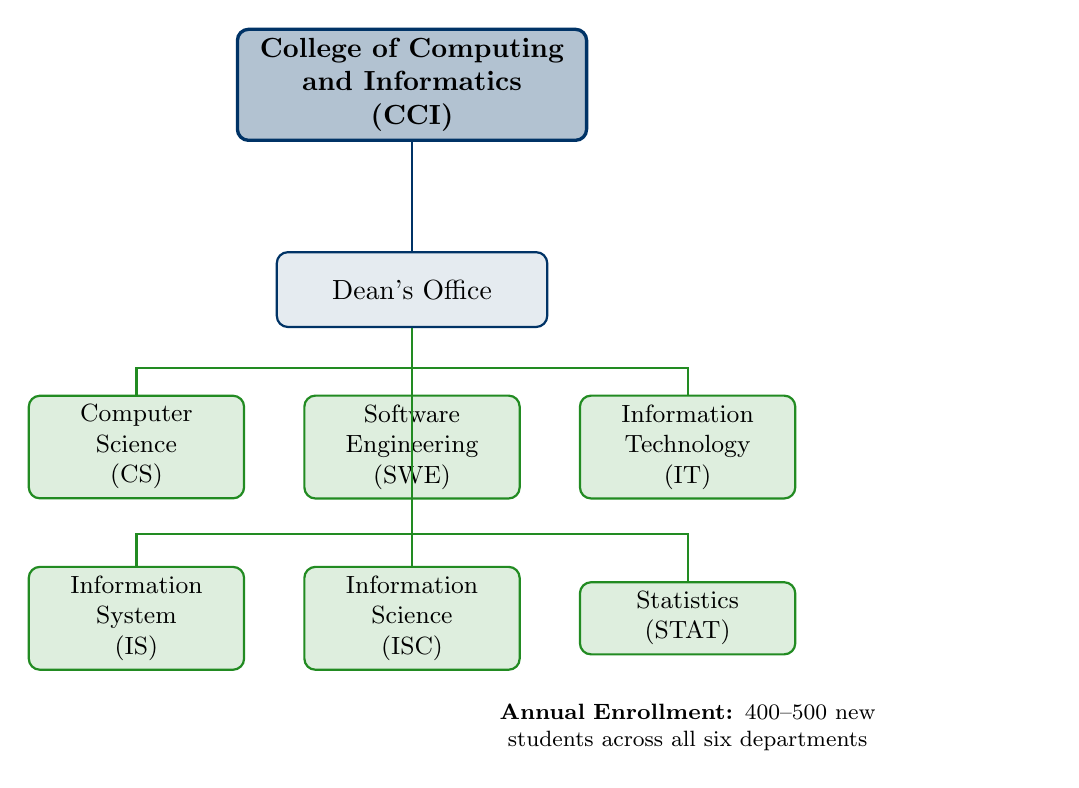
\begin{tikzpicture}[
    box/.style={rectangle, draw=uniblue, thick, fill=uniblue!10, text width=3.2cm, align=center, minimum height=0.95cm, rounded corners},
    deptbox/.style={rectangle, draw=unigreen, thick, fill=unigreen!15, text width=2.5cm, align=center, minimum height=0.85cm, rounded corners, font=\small},
    title/.style={rectangle, draw=uniblue, very thick, fill=uniblue!30, text width=4.2cm, align=center, minimum height=1.1cm, rounded corners, font=\bfseries}
]

% Title
\node[title] (cci) at (0, 0) {College of Computing\\and Informatics\\(CCI)};

% Dean Office - 1.5cm vertical spacing from CCI
\node[box] (dean) at (0, -2.6) {Dean's Office};

% Departments - Row 1 with 1cm horizontal spacing between boxes
% Box width = 2.5cm, so centers are 3.5cm apart (2.5 + 1.0 = 3.5)
\node[deptbox] (cs) at (-3.5, -4.6) {Computer\\Science\\(CS)};
\node[deptbox] (swe) at (0, -4.6) {Software\\Engineering\\(SWE)};
\node[deptbox] (it) at (3.5, -4.6) {Information\\Technology\\(IT)};

% Departments - Row 2 with 1.5cm vertical spacing from Row 1
% Box height = 0.85cm, spacing = 1.5cm, so Row 2 y = -4.6 - 0.85/2 - 1.5 - 0.85/2 = -6.775
\node[deptbox] (is) at (-3.5, -6.775) {Information\\System\\(IS)};
\node[deptbox] (isc) at (0, -6.775) {Information\\Science\\(ISC)};
\node[deptbox] (stat) at (3.5, -6.775) {Statistics\\(STAT)};

% Enrollment info
\node[below=0.5cm of stat, font=\footnotesize, text width=9cm, align=center] (enroll) {
    \textbf{Annual Enrollment:} 400--500 new students across all six departments
};

% Connections from dean to departments
\coordinate (split1) at (0, -3.6);
\coordinate (split2) at (0, -5.7);

\draw[thick, uniblue] (cci) -- (dean);
\draw[thick, unigreen] (dean) -- (split1);

% Row 1 connections
\draw[thick, unigreen] (split1) -| (cs);
\draw[thick, unigreen] (split1) -- (swe);
\draw[thick, unigreen] (split1) -| (it);

% Row 2 connections
\draw[thick, unigreen] (split1) -- (split2);
\draw[thick, unigreen] (split2) -| (is);
\draw[thick, unigreen] (split2) -- (isc);
\draw[thick, unigreen] (split2) -| (stat);

\end{tikzpicture}
\caption{CCI organizational structure showing six specialized departments}
\label{fig:cci-structure}
\end{figure}

The university's ICT Center serves as the primary technical support unit for the institution, managing infrastructure, providing technical training, and supporting innovative student projects. This internship project was conducted under the supervision of the ICT Center during a 6-week intensive development period from \TODO{Start Date} to \TODO{End Date}, 2026. The internship aimed to develop practical software engineering skills while addressing a real institutional challenge: the lack of structured guidance for incoming students selecting their academic departments.

The project team consisted of five Computer Science students working collaboratively under Agile methodology, with weekly supervision meetings, daily standups, and sprint-based deliverables. The team operated within the ICT Center's development environment, utilizing modern cloud-based technologies and following industry-standard software development practices.


Historically, previous attempts to address this placement issue relied heavily on manual advising sessions, printed brochures, and brief introductory seminars during orientation week. While helpful, these analog approaches failed to scale with increasing student enrollment and lacked the personalized, data-driven insights necessary for optimal decision-making. The current status of the topic reveals an urgent need for digital transformation, paving the way for the project detailed herein: the CCI Department Choice Guidance System.

This document serves as a comprehensive record of the software development lifecycle for this guidance system. The report is meticulously organized into six chapters to capture the reader's attention and guide them through the engineering process. Chapter One sets the context with the problem statement and objectives. Chapter Two details the software development plan, including timelines and resource allocation. Chapter Three delves into rigorous requirements analysis, outlining both functional and non-functional specifications. Chapter Four visualizes the system's architecture and design through Data Flow and UML diagrams. Chapter Five provides an in-depth analysis of the system's physical implementation and the quality assurance procedures utilized. Finally, Chapter Six concludes the report with reflections on the internship experience, highlighting key technical learnings and actionable recommendations.


% ─────────────────────────────────────────────────────────────────────────────
\subsection{Statement of the Problem}
% ─────────────────────────────────────────────────────────────────────────────

Despite the critical importance of department selection in shaping students' academic trajectories and career prospects, incoming CCI students at Haramaya University face a significant information gap when making this decision. The current department selection process relies primarily on informal peer advice, limited orientation sessions, and personal assumptions, often leading to mismatched placements and subsequent dissatisfaction.

\subsubsection*{Evidence of the Problem}

A structured survey conducted with 43 current CCI students across all six departments revealed the following:

\begin{itemize}[leftmargin=1.5em, itemsep=3pt]
    \item Only \textbf{55.8\%} of students felt fully confident they understood the differences between departments when making their initial selection
    \item \textbf{97.7\%} of students indicated they would use or seriously consider using a department recommendation tool if one were available
    \item \textbf{41.9\%} of respondents admitted they selected their department based solely on peer recommendations without understanding the curriculum or career implications
    \item Multiple students reported considering or submitting department transfer requests due to mismatched expectations
\end{itemize}

\subsubsection*{Consequences of the Problem}

The absence of a structured guidance system has several negative impacts:

\begin{enumerate}[leftmargin=1.5em, itemsep=3pt]
    \item \textbf{Uninformed Decisions}: Students make critical academic choices without adequate information about department focus areas, curriculum structure, career paths, and skill requirements.
    
    \item \textbf{Mismatched Placements}: Students with strengths in theoretical computer science may end up in applied IT programs, while those interested in business-oriented information systems may find themselves in algorithm-heavy CS courses.
    
    \item \textbf{Transfer Requests and Delays}: Dissatisfied students submit department transfer requests, which create administrative burden and may delay graduation timelines.
    
    \item \textbf{Unbalanced Enrollment}: Without objective guidance, students tend to cluster in perceived "popular" departments (often CS or SWE), leading to overcrowding in some departments and underutilization of resources in others.
    
    \item \textbf{Reduced Retention and Satisfaction}: Students in poorly matched departments experience lower academic satisfaction, reduced motivation, and in some cases, higher dropout rates.
\end{enumerate}

\subsubsection*{Problem Statement}

\begin{tcolorbox}[
    enhanced, colback=lightblue, colframe=uniblue,
    arc=4pt, boxrule=1pt, top=6pt, bottom=6pt, left=8pt, right=8pt
]
\textit{\textbf{Problem Statement:} Incoming CCI students at Haramaya University lack a centralized, evidence-based, and personalized guidance tool to support their department selection decision, resulting in uninformed choices, mismatched placements, administrative burden from transfer requests, unbalanced departmental enrollment, and reduced student satisfaction.}
\end{tcolorbox}

\vspace{6pt}

\subsubsection*{Survey Evidence - Key Statistics}

The survey of 43 CCI students revealed three critical data points that quantify the problem:

\begin{figure}[H]
\centering
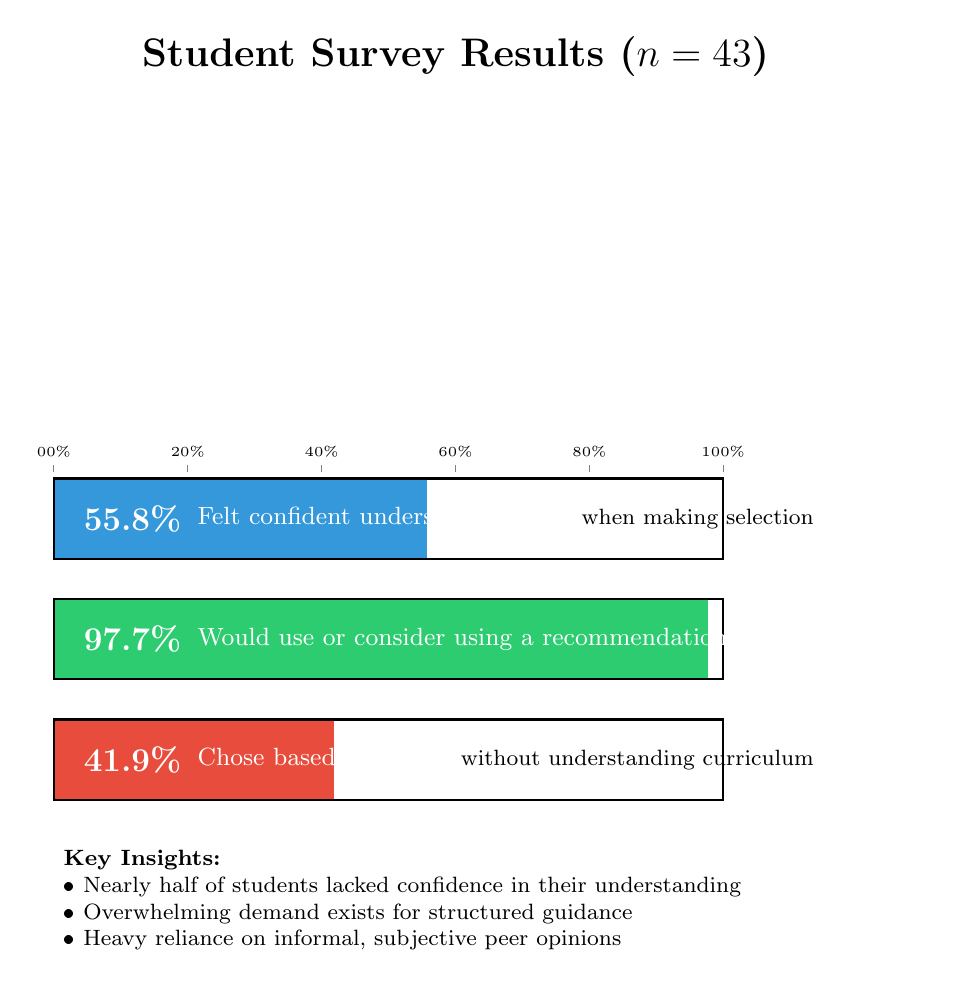
\begin{tikzpicture}[scale=0.85]
    % Define colors
    \definecolor{barcolor1}{RGB}{52, 152, 219}
    \definecolor{barcolor2}{RGB}{46, 204, 113}
    \definecolor{barcolor3}{RGB}{231, 76, 60}
    
    % Chart title
    \node[font=\Large\bfseries] at (6, 7.5) {Student Survey Results ($n = 43$)};
    
    % Bar 1: 55.8% confident
    \fill[barcolor1] (0, 0) rectangle (5.58, 1.2);
    \draw[black, thick] (0, 0) rectangle (10, 1.2);
    \node[anchor=west, font=\large\bfseries, white] at (0.3, 0.6) {55.8\%};
    \node[anchor=west, font=\small, white] at (2, 0.6) {Felt confident understanding departments};
    \node[anchor=east, font=\footnotesize] at (11.5, 0.6) {when making selection};
    
    % Bar 2: 97.7% would use tool
    \fill[barcolor2] (0, -1.8) rectangle (9.77, -0.6);
    \draw[black, thick] (0, -1.8) rectangle (10, -0.6);
    \node[anchor=west, font=\large\bfseries, white] at (0.3, -1.2) {97.7\%};
    \node[anchor=west, font=\small, white] at (2, -1.2) {Would use or consider using a recommendation tool};
    
    % Bar 3: 41.9% peer-based
    \fill[barcolor3] (0, -3.6) rectangle (4.19, -2.4);
    \draw[black, thick] (0, -3.6) rectangle (10, -2.4);
    \node[anchor=west, font=\large\bfseries, white] at (0.3, -3) {41.9\%};
    \node[anchor=west, font=\small, white] at (2, -3) {Chose based solely on peer advice};
    \node[anchor=east, font=\footnotesize] at (11.5, -3) {without understanding curriculum};
    
    % Scale markers
    \foreach \x in {0, 2, 4, 6, 8, 10} {
        \draw[gray, thin] (\x, 1.4) -- (\x, 1.3);
        \node[font=\tiny] at (\x, 1.6) {\x 0\%};
    }
    
    % Legend
    \node[anchor=west, font=\footnotesize\bfseries] at (0, -4.5) {Key Insights:};
    \node[anchor=west, font=\footnotesize, text width=11cm, align=left] at (0, -5.3) {
        • Nearly half of students lacked confidence in their understanding\\
        • Overwhelming demand exists for structured guidance\\
        • Heavy reliance on informal, subjective peer opinions
    };
\end{tikzpicture}
\caption{Survey results highlighting the need for a department guidance system}
\label{fig:survey-results}
\end{figure}

\subsubsection*{Scope of the Solution}

This project addresses the problem by developing a web-based \textbf{CCI Department Choice Guidance System} that:

\begin{itemize}[leftmargin=1.5em, itemsep=3pt]
    \item Presents students with a structured 20-question assessment covering interests, skills, career goals, and learning preferences
    \item Applies a weighted scoring algorithm validated by department heads to compute match percentages for all six departments
    \item Provides ranked recommendations with AI-generated explanations tailored to individual response patterns
    \item Offers comprehensive department profiles including curriculum focus, career paths, required skills, and common misconceptions
    \item Enables side-by-side comparison of top recommended departments
    \item Allows students to export personalized reports as PDF for future reference
    \item Provides administrators with analytics on usage patterns and departmental interest trends
\end{itemize}

% ─────────────────────────────────────────────────────────────────────────────
\subsection{Objectives}
% ─────────────────────────────────────────────────────────────────────────────

\subsubsection*{General Objective}

To design, develop, and deploy a web-based department recommendation system that guides incoming CCI students at Haramaya University in making informed, evidence-based department selection decisions by providing personalized assessments, ranked recommendations, and comprehensive department information.

\subsubsection*{Specific Objectives}

\begin{enumerate}[leftmargin=1.5em, itemsep=4pt]
    \item \textbf{Requirements Gathering and Validation}  
    Conduct a structured survey of current CCI students (target: $n \geq 40$) and consult with department heads to validate the problem, gather department-specific criteria, and identify key decision factors that differentiate the six departments.
    
    \item \textbf{Assessment Questionnaire Design}  
    Design and implement a 20-question interactive assessment questionnaire that evaluates student interests, technical aptitudes, career aspirations, learning preferences, and problem-solving approaches, with response options mapped to department-specific scoring weights.
    
    \item \textbf{Scoring Algorithm Development}  
    Develop a weighted scoring algorithm using HOD-validated criteria to compute match scores for all six CCI departments (CS, SWE, IT, IS, ISC, STAT), ensuring the algorithm produces differentiated and meaningful recommendations rather than similar scores across departments.
    
    \item \textbf{AI-Powered Explanation Generation}  
    Integrate an LLM API (OpenAI GPT or Google Gemini) to generate personalized recommendation explanations based on individual response patterns, with a template-based fallback system for cases where API calls fail or timeout.
    
    \item \textbf{Department Information Repository}  
    Build a comprehensive department information repository with structured profiles for all six departments covering core focus areas, curriculum highlights, typical career outcomes, required skills, and common misconceptions, sourced from official university documentation and HOD interviews.
    
    \item \textbf{Administrative Dashboard}  
    Develop an administrative dashboard with role-based access control enabling authorized users (ICT Center staff, HODs) to manage department content, update the question bank, review usage analytics, and export aggregated data for enrollment planning.
    
    \item \textbf{Cloud Deployment and Reliability}  
    Deploy the system to free-tier cloud infrastructure (Vercel for frontend, Render for backend, MongoDB Atlas for database) within the 6-week development timeline, achieving 99\%+ uptime and sub-2-second response times for the recommendation engine.
    
    \item \textbf{User Adoption and Satisfaction}  
    Achieve a minimum 70\% usage rate among incoming CCI students within the first enrollment period and maintain an 80\%+ user satisfaction rating based on post-assessment feedback surveys.
\end{enumerate}

\subsection{Scope and Limitation of the Project}

\subsubsection*{Project Scope}

The CCI Department Choice Guidance System covers the following functional and operational boundaries:

\paragraph{Functional Scope (In-Scope Features)}

\begin{itemize}[leftmargin=1.5em, itemsep=3pt]
    \item \textbf{Interactive Assessment Module}: 20-question assessment covering interests, aptitudes, career goals, learning styles, and problem-solving approaches with multiple-choice responses
    
    \item \textbf{Weighted Recommendation Engine}: Algorithm using HOD-validated scoring weights to compute match percentages for all six CCI departments (CS, SWE, IT, IS, ISC, STAT)
    
    \item \textbf{AI-Powered Explanations}: Integration with LLM API (OpenAI GPT-3.5 or Google Gemini) to generate personalized recommendation narratives based on individual response patterns
    
    \item \textbf{Department Information Repository}: Comprehensive profiles for all six departments including curriculum focus, career paths, required skills, common misconceptions, and sample projects
    
    \item \textbf{Department Comparison Feature}: Side-by-side comparison view for top 3 recommended departments with key differentiators highlighted
    
    \item \textbf{PDF Export Functionality}: Downloadable personalized report containing assessment results, recommendations, explanations, and department profiles for offline reference
    
    \item \textbf{Administrative Dashboard}: Secure admin interface for content management (department profiles, questions), analytics viewing (usage statistics, departmental interest trends), and data export
    
    \item \textbf{Anonymous Student Access}: No authentication required for students; session-based tracking with 30-day auto-deletion of response data
    
    \item \textbf{Responsive Web Design}: Mobile-first design ensuring usability on smartphones, tablets, and desktop computers
    
    \item \textbf{Basic Analytics}: Aggregated usage statistics including completion rates, departmental interest distribution, and average assessment duration
\end{itemize}

\paragraph{Operational Scope}

\begin{itemize}[leftmargin=1.5em, itemsep=3pt]
    \item \textbf{Target Users}: Incoming CCI students (primary), ICT Center administrators (secondary), department heads (view-only access)
    \item \textbf{Geographic Scope}: Haramaya University CCI students (initially); system architecture supports future expansion
    \item \textbf{Deployment Environment}: Cloud-hosted (Vercel + Render + MongoDB Atlas) accessible via web browser
    \item \textbf{Development Timeline}: 6-week intensive development period (Week 1: Requirements, Week 2-3: Design \& Backend, Week 4-5: Frontend \& Integration, Week 6: Testing \& Deployment)
    \item \textbf{Technology Constraints}: Free-tier cloud services, open-source frameworks, publicly accessible LLM APIs
\end{itemize}

\subsubsection*{Project Limitations}

The following features and functionalities are explicitly excluded from the current project scope:

\paragraph{Technical Limitations}

\begin{itemize}[leftmargin=1.5em, itemsep=3pt]
    \item \textbf{No Native Mobile Apps}: System delivered as responsive web application; no iOS or Android native apps developed
    
    \item \textbf{No Amharic Language Support}: Interface and content provided in English only; internationalization not implemented
    
    \item \textbf{No University System Integration}: No direct integration with Haramaya University's student registration system, course management system, or student information system
    
    \item \textbf{No Real-Time Collaboration}: Students cannot save partial assessments or collaborate with peers in real-time
    
    \item \textbf{Limited AI Context}: LLM explanations based solely on questionnaire responses; no access to student academic records, entrance exam scores, or prior coursework
    
    \item \textbf{No Video Content}: Department information presented via text and images only; no video tutorials, department tours, or student testimonials
\end{itemize}

\paragraph{Functional Limitations}

\begin{itemize}[leftmargin=1.5em, itemsep=3pt]
    \item \textbf{No Live Chat Support}: No real-time help desk or chatbot for student questions; static FAQ provided instead
    
    \item \textbf{No Aptitude Testing}: Assessment based on self-reported interests and preferences; no programming tests, logic puzzles, or skill validation exercises
    
    \item \textbf{No Course-Level Recommendations}: System recommends departments only; does not suggest specific courses, electives, or academic pathways
    
    \item \textbf{No Career Counseling}: Provides career path information but does not offer personalized career counseling or industry connections
    
    \item \textbf{No Historical Data Analysis}: Recommendations based on current criteria only; no predictive modeling using historical student placement outcomes
\end{itemize}

\paragraph{Data and Privacy Limitations}

\begin{itemize}[leftmargin=1.5em, itemsep=3pt]
    \item \textbf{Anonymous Data Only}: System does not collect student names, IDs, email addresses, or other personally identifiable information
    
    \item \textbf{30-Day Data Retention}: Student response data automatically deleted after 30 days; no long-term tracking or longitudinal studies
    
    \item \textbf{No Integration with Academic Records}: Cannot access or consider student GPA, entrance exam scores, or prior academic performance
\end{itemize}

\paragraph{Scalability and Performance Limitations}

\begin{itemize}[leftmargin=1.5em, itemsep=3pt]
    \item \textbf{Free-Tier Infrastructure}: System hosted on free-tier cloud services with monthly usage limits (bandwidth, compute hours, database storage)
    
    \item \textbf{Concurrent User Limit}: Designed to handle 50 concurrent users; performance degradation expected beyond this threshold
    
    \item \textbf{LLM API Rate Limits}: AI explanation generation subject to third-party API rate limits; fallback to template-based explanations when limits exceeded
\end{itemize}

% ─────────────────────────────────────────────────────────────────────────────
\subsection{Significance of the Project}
% ─────────────────────────────────────────────────────────────────────────────

The CCI Department Choice Guidance System addresses a critical gap in the student onboarding process and delivers value to multiple stakeholders within the Haramaya University ecosystem.

\subsubsection*{Significance for Students}

\begin{itemize}[leftmargin=1.5em, itemsep=3pt]
    \item \textbf{Informed Decision-Making}: Students receive evidence-based, personalized recommendations rather than relying on peer advice or assumptions, reducing the risk of mismatched department placements.
    
    \item \textbf{Reduced Uncertainty and Anxiety}: A structured assessment process provides clarity and confidence during the stressful department selection period, replacing ambiguity with actionable guidance.
    
    \item \textbf{Improved Academic Satisfaction}: Students placed in departments aligned with their interests and aptitudes are more likely to experience academic success, higher motivation, and greater satisfaction throughout their degree programs.
    
    \item \textbf{Career Clarity}: Comprehensive department profiles with career path information help students understand long-term professional implications of their department choice.
    
    \item \textbf{Accessible 24/7}: Web-based system allows students to complete assessments at their own pace, revisit department information, and share results with family members for discussion.
\end{itemize}

\subsubsection*{Significance for Haramaya University CCI}

\begin{itemize}[leftmargin=1.5em, itemsep=3pt]
    \item \textbf{Reduced Transfer Requests}: Evidence-based initial placements reduce administrative burden associated with processing department transfer requests.
    
    \item \textbf{Balanced Enrollment}: System promotes awareness of all six departments, potentially distributing students more evenly rather than clustering in perceived "popular" departments.
    
    \item \textbf{Data-Driven Insights}: Analytics dashboard provides administrators with real-time visibility into student interest trends, enabling proactive enrollment planning and resource allocation.
    
    \item \textbf{Enhanced Institutional Image}: Demonstrates CCI's commitment to student success and adoption of modern, technology-driven student services.
    
    \item \textbf{Standardized Onboarding}: Replaces ad-hoc orientation sessions with consistent, repeatable, and scalable guidance process for all incoming students.
\end{itemize}

\subsubsection*{Significance for Department Heads}

\begin{itemize}[leftmargin=1.5em, itemsep=3pt]
    \item \textbf{Better-Matched Students}: Departments receive students whose interests and aptitudes align with departmental focus, improving classroom engagement and reducing early-stage attrition.
    
    \item \textbf{Enrollment Forecasting}: Early visibility into student interest trends enables departments to plan faculty allocation, lab resources, and course offerings more effectively.
    
    \item \textbf{Departmental Visibility}: System ensures all departments (including smaller or less well-known ones like Information Science and Statistics) receive equal exposure and consideration.
    
    \item \textbf{Reduced Advising Burden}: HODs spend less time responding to basic "what's the difference between departments?" questions, freeing time for substantive academic advising.
\end{itemize}

\subsubsection*{Significance for Software Engineering Education}

\begin{itemize}[leftmargin=1.5em, itemsep=3pt]
    \item \textbf{Real-World Problem Solving}: Project team gained hands-on experience addressing a genuine institutional challenge with measurable impact, bridging the gap between academic coursework and professional software development.
    
    \item \textbf{Full-Stack Development Practice}: Team members developed proficiency across frontend (React), backend (Node.js/Express), database (MongoDB), cloud deployment (Vercel/Render), and AI integration (LLM APIs).
    
    \item \textbf{Agile Methodology Application}: Six-week sprint-based development with daily standups, weekly retrospectives, and iterative delivery provided practical Agile/Scrum experience.
    
    \item \textbf{Collaborative Software Engineering}: Five-person team managed through Git version control, code reviews, merge conflicts, and distributed task coordination.
    
    \item \textbf{Stakeholder Engagement}: Direct collaboration with ICT Center supervisors, department heads, and student survey participants simulated real client relationships and requirements gathering.
\end{itemize}

\subsubsection*{Broader Academic Significance}

\begin{itemize}[leftmargin=1.5em, itemsep=3pt]
    \item \textbf{Replicable Model}: System architecture and implementation approach can be adapted by other universities facing similar department selection challenges, particularly in Ethiopia and East Africa.
    
    \item \textbf{Open-Source Contribution Potential}: Codebase structured for potential open-source release, enabling other institutions to customize and deploy similar systems.
    
    \item \textbf{Research Foundation}: Project generates data on student preferences, departmental perceptions, and recommendation algorithm effectiveness, providing foundation for future educational research.
    
    \item \textbf{AI in Education Example}: Demonstrates practical, ethical application of large language models in educational decision support systems.
\end{itemize}

% ─────────────────────────────────────────────────────────────────────────────
\subsection{Methodology}
% ─────────────────────────────────────────────────────────────────────────────

The CCI Department Choice Guidance System was developed using a systematic, Agile-based software development methodology over a 6-week period. The methodology integrated requirements engineering, iterative design and development, stakeholder engagement, and continuous testing.

\subsubsection*{Overall Approach}

The project followed a \textbf{hybrid Agile-Scrum framework} with weekly sprints, daily standups, and iterative delivery. The 6-week timeline was divided into overlapping phases to maximize efficiency:

\begin{itemize}[leftmargin=1.5em, itemsep=3pt]
    \item \textbf{Week 1--2}: Requirements Gathering and System Design
    \item \textbf{Week 2--4}: Backend Development and Database Implementation
    \item \textbf{Week 3--5}: Frontend Development and AI Integration
    \item \textbf{Week 5}: System Integration and Testing
    \item \textbf{Week 6}: Deployment, Documentation, and Handover
\end{itemize}

\subsubsection*{Phase 1: Requirements Gathering and Analysis (Week 1--2)}

\paragraph{Student Survey}
\begin{itemize}[leftmargin=1.5em, itemsep=3pt]
    \item \textbf{Method}: Online structured survey distributed to current CCI students across all six departments via Google Forms
    \item \textbf{Sample Size}: 43 respondents (target: $n \geq 40$)
    \item \textbf{Survey Content}: Department selection experience, information sources used, confidence in choice, willingness to use recommendation tool, satisfaction with current placement
    \item \textbf{Analysis}: Quantitative analysis using descriptive statistics; qualitative analysis of open-ended responses to identify common themes
    \item \textbf{Outcome}: Validated problem statement; identified key decision factors (career paths, curriculum focus, technical vs. theoretical emphasis)
\end{itemize}

\paragraph{Department Head Consultations}
\begin{itemize}[leftmargin=1.5em, itemsep=3pt]
    \item \textbf{Method}: Semi-structured interviews with HODs or senior faculty from each of the six departments
    \item \textbf{Interview Guide}: Department philosophy, core curriculum, typical student profile, common misconceptions, desired student characteristics
    \item \textbf{Question Weight Validation}: Collaborated with HODs to assign scoring weights for questionnaire responses (e.g., "theoretical algorithm interest" scores higher for CS than IT)
    \item \textbf{Outcome}: Validated scoring algorithm weights; gathered authoritative department profiles; identified key differentiators between departments
\end{itemize}

\paragraph{Requirements Documentation}
\begin{itemize}[leftmargin=1.5em, itemsep=3pt]
    \item Documented 12 functional requirements (FR-01 through FR-12) covering assessment, recommendation, comparison, PDF export, and admin functions
    \item Documented 13 non-functional requirements (NFR-01 through NFR-13) covering performance, security, usability, accessibility, and legal compliance
    \item Created user stories and acceptance criteria for each feature
\end{itemize}

\subsubsection*{Phase 2: System Design (Week 2--3)}

\paragraph{Architecture Design}
\begin{itemize}[leftmargin=1.5em, itemsep=3pt]
    \item \textbf{Architectural Pattern}: 3-tier architecture (Client -- Server -- Database) with RESTful API communication
    \item \textbf{Technology Selection}: React (frontend), Node.js/Express (backend), MongoDB Atlas (database), Vercel (frontend hosting), Render (backend hosting)
    \item \textbf{Justification}: Free-tier availability, team familiarity, industry relevance, scalability potential
\end{itemize}

\paragraph{Data Modeling}
\begin{itemize}[leftmargin=1.5em, itemsep=3pt]
    \item Designed MongoDB collections: \texttt{departments}, \texttt{questions}, \texttt{sessions}, \texttt{adminUsers}, \texttt{analytics}
    \item Defined schema for 20-question assessment with per-department scoring weights
    \item Structured department profiles with focus areas, career paths, curriculum highlights
\end{itemize}

\paragraph{System Modeling}
\begin{itemize}[leftmargin=1.5em, itemsep=3pt]
    \item \textbf{Data Flow Diagrams}: Created Level 0 (context), Level 1 (6 main processes), and Level 2 (Process 3 decomposition) DFDs
    \item \textbf{Activity Diagram}: Modeled student assessment workflow from start to PDF export
    \item \textbf{UI Wireframes}: Sketched low-fidelity mockups for assessment page, results page, comparison view, and admin dashboard
\end{itemize}

\subsubsection*{Phase 3: Implementation (Week 2--5)}

\paragraph{Backend Development (Week 2--4)}
\begin{itemize}[leftmargin=1.5em, itemsep=3pt]
    \item Implemented Express.js REST API with endpoints for assessment submission, recommendation retrieval, department data, admin operations
    \item Developed weighted scoring algorithm: $\text{Score}_{\text{dept}} = \sum_{i=1}^{20} w_{i,\text{dept}} \times r_i$ where $w$ = question weight, $r$ = student response
    \item Integrated MongoDB with Mongoose ODM for data persistence
    \item Implemented JWT-based authentication for admin dashboard
    \item Integrated OpenAI GPT-3.5 API for explanation generation with 5-second timeout and template fallback
\end{itemize}

\paragraph{Frontend Development (Week 3--5)}
\begin{itemize}[leftmargin=1.5em, itemsep=3pt]
    \item Built responsive React components for assessment UI, progress indicator, results visualization, department comparison
    \item Implemented state management using React Context API
    \item Developed PDF export functionality using jsPDF library
    \item Created admin dashboard with content management forms and analytics charts
    \item Applied CSS Flexbox and Grid for responsive mobile-first design
\end{itemize}

\paragraph{Integration (Week 5)}
\begin{itemize}[leftmargin=1.5em, itemsep=3pt]
    \item Connected frontend React app to backend Express API via Axios HTTP client
    \item Tested end-to-end workflows: assessment submission, recommendation retrieval, PDF generation
    \item Implemented error handling for API failures, network errors, LLM timeouts
    \item Integrated analytics tracking for usage statistics
\end{itemize}

\subsubsection*{Phase 4: Testing and Quality Assurance (Week 5--6)}

\paragraph{Unit Testing}
\begin{itemize}[leftmargin=1.5em, itemsep=3pt]
    \item Backend: Tested scoring algorithm with edge cases (all same answers, conflicting responses)
    \item Frontend: Tested form validation, state transitions, PDF generation
\end{itemize}

\paragraph{Integration Testing}
\begin{itemize}[leftmargin=1.5em, itemsep=3pt]
    \item End-to-end testing of assessment submission and recommendation retrieval
    \item LLM API failure scenarios (timeout, rate limit, invalid response)
    \item Database operations (CRUD for questions, departments, admin users)
\end{itemize}

\paragraph{User Acceptance Testing}
\begin{itemize}[leftmargin=1.5em, itemsep=3pt]
    \item Pilot testing with 10 volunteer CCI students
    \item Collected feedback on UI clarity, question comprehensibility, recommendation usefulness
    \item Iteratively refined based on usability feedback
\end{itemize}

\paragraph{Cross-Browser and Device Testing}
\begin{itemize}[leftmargin=1.5em, itemsep=3pt]
    \item Tested on Chrome, Firefox, Safari, Edge browsers
    \item Verified responsive design on mobile (iOS/Android), tablet, and desktop screen sizes
\end{itemize}

\subsubsection*{Phase 5: Deployment and Handover (Week 6)}

\paragraph{Cloud Deployment}
\begin{itemize}[leftmargin=1.5em, itemsep=3pt]
    \item Frontend deployed to Vercel with automatic CI/CD from GitHub main branch
    \item Backend deployed to Render with environment variable configuration for API keys and database connection
    \item MongoDB Atlas cluster configured with IP whitelist and database user credentials
    \item Custom domain configured (if applicable) or deployed to default Vercel/Render URLs
\end{itemize}

\paragraph{Documentation}
\begin{itemize}[leftmargin=1.5em, itemsep=3pt]
    \item User documentation: How to complete assessment, interpret results, export PDF
    \item Admin documentation: How to login, update content, view analytics
    \item Technical documentation: System architecture, API endpoints, database schema, deployment instructions
    \item Internship report: This comprehensive document following Haramaya University Industrial Practice Report guidelines
\end{itemize}

\paragraph{Handover to ICT Center}
\begin{itemize}[leftmargin=1.5em, itemsep=3pt]
    \item Demonstration session with ICT Center supervisors
    \item Transfer of admin credentials, API keys, and cloud account access
    \item Knowledge transfer session on system maintenance and content updates
    \item Codebase transfer via GitHub repository with README instructions
\end{itemize}

\subsubsection*{Tools and Technologies Used}

\begin{table}[H]
\centering
\small
\begin{tabularx}{\textwidth}{>{\raggedright\arraybackslash}p{3.5cm}>{\raggedright\arraybackslash}p{3cm}>{\raggedright\arraybackslash}X}
\toprule
\theadrow
\textbf{Category} & \textbf{Tool/Technology} & \textbf{Purpose} \\
\midrule
Frontend Framework & React 18.x & Component-based UI development \\[3pt]
\rowalt
Backend Framework & Node.js + Express & REST API server \\[3pt]
Database & MongoDB Atlas & NoSQL cloud database \\[3pt]
\rowalt
AI Integration & OpenAI GPT-3.5 API & Recommendation explanations \\[3pt]
Version Control & Git + GitHub & Code management and collaboration \\[3pt]
\rowalt
Frontend Hosting & Vercel & Serverless deployment \\[3pt]
Backend Hosting & Render & Container-based API hosting \\[3pt]
\rowalt
IDE & VS Code & Development environment \\[3pt]
API Testing & Postman & Backend endpoint testing \\[3pt]
\rowalt
Project Management & GitHub Projects & Task tracking and sprint planning \\[3pt]
Communication & WhatsApp + Email & Team coordination \\[3pt]
\rowalt
Documentation & LaTeX + Markdown & Report writing \\[3pt]
\bottomrule
\end{tabularx}
\caption{Development tools and technologies}
\end{table}

\subsubsection*{Team Collaboration and Roles}

The five-member development team operated under Agile principles:

\begin{itemize}[leftmargin=1.5em, itemsep=3pt]
    \item \textbf{Daily Standups}: 15-minute virtual meetings to share progress, blockers, and daily goals
    \item \textbf{Weekly Sprints}: Sunday sprint planning, Friday sprint review and retrospective
    \item \textbf{Code Reviews}: All pull requests reviewed by at least one team member before merging
    \item \textbf{Pair Programming}: Complex features (scoring algorithm, LLM integration) developed collaboratively
    \item \textbf{Documentation}: Each team member documented their code and contributed to final report
\end{itemize}

Team roles aligned with individual strengths while ensuring cross-functional learning opportunities.

% ─────────────────────────────────────────────────────────────────────────────
\subsubsection{System Development Methodology}
% ─────────────────────────────────────────────────────────────────────────────

The project adopted an \textbf{Agile-Scrum framework} tailored for a 6-week intensive development cycle. This methodology was selected for its iterative approach, flexibility in responding to changing requirements, and emphasis on working software delivery.

\paragraph{Agile Principles Applied}

\begin{itemize}[leftmargin=1.5em, itemsep=3pt]
    \item \textbf{Iterative Development}: System built incrementally through weekly sprints, with each sprint producing a potentially shippable product increment
    
    \item \textbf{Continuous Feedback}: Weekly demonstrations to ICT Center supervisors enabled early course correction and requirement clarification
    
    \item \textbf{Self-Organizing Team}: Five-member team collaboratively assigned tasks based on individual expertise and learning goals
    
    \item \textbf{Working Software Focus}: Emphasis on functional prototypes over comprehensive documentation; documentation produced in parallel with development
    
    \item \textbf{Adaptive Planning}: Sprint goals adjusted based on technical discoveries, stakeholder feedback, and API integration challenges
\end{itemize}

\paragraph{Sprint Structure}

Each one-week sprint followed this cadence:

\begin{enumerate}[leftmargin=1.5em, itemsep=3pt]
    \item \textbf{Sunday: Sprint Planning} (2 hours)
    \begin{itemize}[leftmargin=1.5em, itemsep=2pt]
        \item Review previous sprint outcomes
        \item Select user stories for current sprint from product backlog
        \item Break down stories into tasks with time estimates
        \item Assign tasks based on team member availability and expertise
    \end{itemize}
    
    \item \textbf{Monday--Thursday: Daily Development} with 15-minute standups
    \begin{itemize}[leftmargin=1.5em, itemsep=2pt]
        \item What did I complete yesterday?
        \item What will I work on today?
        \item Are there any blockers?
    \end{itemize}
    
    \item \textbf{Friday: Sprint Review \& Retrospective} (2 hours)
    \begin{itemize}[leftmargin=1.5em, itemsep=2pt]
        \item Demonstrate completed features to stakeholders
        \item Accept/reject user stories based on acceptance criteria
        \item Team retrospective: What went well? What needs improvement?
        \item Update product backlog priorities
    \end{itemize}
\end{enumerate}

\paragraph{Development Practices}

\begin{itemize}[leftmargin=1.5em, itemsep=3pt]
    \item \textbf{Version Control}: Git with feature branch workflow; all code merged via pull requests
    \item \textbf{Code Reviews}: Minimum one team member approval before merging to main branch
    \item \textbf{Pair Programming}: Applied for complex modules (scoring algorithm, LLM API integration)
    \item \textbf{Continuous Integration}: Automated builds triggered on every commit to main branch
    \item \textbf{Definition of Done}: Feature complete, unit tested, code reviewed, documented, deployed to staging
\end{itemize}

% ─────────────────────────────────────────────────────────────────────────────
\subsubsection{Data Collection Methods}
% ─────────────────────────────────────────────────────────────────────────────

The project employed multiple data collection methods to ensure requirements were grounded in empirical evidence and stakeholder input.

\paragraph{1. Student Survey (Quantitative + Qualitative)}

\begin{itemize}[leftmargin=1.5em, itemsep=3pt]
    \item \textbf{Instrument}: Structured online questionnaire via Google Forms
    \item \textbf{Target Population}: Current CCI students across all six departments (CS, SWE, IT, IS, ISC, STAT)
    \item \textbf{Sampling Method}: Convenience sampling; survey link distributed via department WhatsApp groups and email lists
    \item \textbf{Sample Size}: 43 respondents (target: $n \geq 40$)
    \item \textbf{Response Rate}: Approximately 12\% of total CCI student population
    \item \textbf{Survey Sections}:
    \begin{enumerate}[leftmargin=1.5em, itemsep=2pt]
        \item Demographics (current department, year of study)
        \item Department selection experience (How did you choose? What information sources?)
        \item Confidence and satisfaction (5-point Likert scale)
        \item Information needs (What information would have been helpful?)
        \item Tool willingness (Would you use a recommendation system? Why/why not?)
        \item Open-ended suggestions
    \end{enumerate}
    \item \textbf{Analysis Methods}:
    \begin{itemize}[leftmargin=1.5em, itemsep=2pt]
        \item Descriptive statistics (percentages, means) for quantitative responses
        \item Thematic analysis for open-ended text responses
        \item Cross-tabulation by department to identify patterns
    \end{itemize}
    \item \textbf{Key Findings}:
    \begin{itemize}[leftmargin=1.5em, itemsep=2pt]
        \item 55.8\% felt confident in understanding department differences
        \item 97.7\% would use or consider using a recommendation tool
        \item 41.9\% chose based primarily on peer advice
        \item Top requested information: career paths, curriculum details, skill requirements
    \end{itemize}
\end{itemize}

\paragraph{2. Department Head Interviews (Qualitative)}

\begin{itemize}[leftmargin=1.5em, itemsep=3pt]
    \item \textbf{Method}: Semi-structured interviews with HODs or senior faculty representatives
    \item \textbf{Participants}: Representatives from all six CCI departments
    \item \textbf{Interview Duration}: 30--45 minutes per department
    \item \textbf{Interview Guide Topics}:
    \begin{enumerate}[leftmargin=1.5em, itemsep=2pt]
        \item Department philosophy and core focus
        \item Typical successful student profile (interests, skills, mindset)
        \item Common student misconceptions about the department
        \item Key differentiators from similar departments
        \item Curriculum highlights and unique courses
        \item Career outcomes and industry connections
        \item Desired characteristics in incoming students
    \end{enumerate}
    \item \textbf{Data Recording}: Handwritten notes; key quotes documented
    \item \textbf{Validation Activity}: HODs reviewed and validated scoring weights for questionnaire responses
    \item \textbf{Output}: Authoritative department profiles; validated recommendation algorithm weights
\end{itemize}

\paragraph{3. Existing System Analysis (Document Review)}

\begin{itemize}[leftmargin=1.5em, itemsep=3pt]
    \item \textbf{Sources Reviewed}:
    \begin{itemize}[leftmargin=1.5em, itemsep=2pt]
        \item Official CCI department pages on Haramaya University website
        \item Course catalogs and curriculum documents
        \item Student orientation materials
        \item Department brochures (where available)
    \end{itemize}
    \item \textbf{Purpose}: Identify gaps in current information provision; extract structured department data
    \item \textbf{Findings}: Minimal online department comparison resources; no interactive tools; information scattered across multiple documents
\end{itemize}

\paragraph{4. Technical Data Sources}

\begin{itemize}[leftmargin=1.5em, itemsep=3pt]
    \item \textbf{Question Bank Design}: Questions iteratively drafted by team, reviewed by ICT supervisors, validated by HODs
    \item \textbf{Scoring Weights}: Department-specific weights (0--3 scale) assigned collaboratively with HODs to each questionnaire response option
    \item \textbf{Department Profiles}: Structured data extracted from official sources, supplemented by HOD interviews
\end{itemize}

% ─────────────────────────────────────────────────────────────────────────────
\subsubsection{System Development Tools}
% ─────────────────────────────────────────────────────────────────────────────

The project utilized modern, industry-standard tools and technologies selected for their suitability to project requirements, team familiarity, free-tier availability, and learning value.

\paragraph{Development Environment}

\begin{itemize}[leftmargin=1.5em, itemsep=3pt]
    \item \textbf{IDE}: Visual Studio Code 1.85+ with extensions (ESLint, Prettier, GitLens, MongoDB for VS Code)
    \item \textbf{Operating Systems}: Windows 10/11 (primary); Linux Ubuntu 22.04 (testing)
    \item \textbf{Terminal}: Git Bash (Windows); native terminal (Linux)
\end{itemize}

\paragraph{Frontend Technologies}

\begin{itemize}[leftmargin=1.5em, itemsep=3pt]
    \item \textbf{Framework}: React 18.2.0 (component-based UI library)
    \item \textbf{Build Tool}: Vite 4.x (fast build tool and dev server)
    \item \textbf{Styling}: CSS3 with Flexbox and Grid; custom CSS variables for theming
    \item \textbf{HTTP Client}: Axios 1.x (promise-based HTTP requests)
    \item \textbf{PDF Generation}: jsPDF 2.x (client-side PDF creation)
    \item \textbf{State Management}: React Context API (lightweight global state)
    \item \textbf{Routing}: React Router 6.x (client-side navigation)
\end{itemize}

\paragraph{Backend Technologies}

\begin{itemize}[leftmargin=1.5em, itemsep=3pt]
    \item \textbf{Runtime}: Node.js 18.x LTS
    \item \textbf{Framework}: Express.js 4.x (web application framework)
    \item \textbf{Database}: MongoDB 6.0 via MongoDB Atlas (cloud-hosted NoSQL database)
    \item \textbf{ODM}: Mongoose 7.x (MongoDB object modeling for Node.js)
    \item \textbf{Authentication}: JSON Web Tokens (JWT) via \texttt{jsonwebtoken} package
    \item \textbf{Password Hashing}: bcrypt 5.x (secure password hashing)
    \item \textbf{Environment Variables}: dotenv (configuration management)
    \item \textbf{CORS}: cors package (cross-origin resource sharing)
\end{itemize}

\paragraph{AI Integration}

\begin{itemize}[leftmargin=1.5em, itemsep=3pt]
    \item \textbf{LLM API}: OpenAI GPT-3.5-turbo via official OpenAI Node.js SDK
    \item \textbf{API Key Management}: Environment variable with fallback template system
    \item \textbf{Timeout Handling}: 5-second maximum wait time with graceful fallback
    \item \textbf{Prompt Engineering}: Structured prompt templates for consistent output format
\end{itemize}

\paragraph{Version Control \& Collaboration}

\begin{itemize}[leftmargin=1.5em, itemsep=3pt]
    \item \textbf{Version Control}: Git 2.40+
    \item \textbf{Repository Hosting}: GitHub (private repository)
    \item \textbf{Branching Strategy}: Feature branch workflow (\texttt{main}, \texttt{develop}, \texttt{feature/*}, \texttt{bugfix/*})
    \item \textbf{Project Management}: GitHub Projects (Kanban board for task tracking)
    \item \textbf{Communication}: WhatsApp (daily coordination); Email (formal communications)
\end{itemize}

\paragraph{Testing Tools}

\begin{itemize}[leftmargin=1.5em, itemsep=3pt]
    \item \textbf{API Testing}: Postman (endpoint testing and documentation)
    \item \textbf{Browser Testing}: Chrome DevTools, Firefox Developer Tools
    \item \textbf{Responsive Testing}: Chrome DevTools device emulation; physical mobile devices
    \item \textbf{Manual Testing}: Structured test cases in Google Sheets
\end{itemize}

\paragraph{Deployment \& Hosting}

\begin{itemize}[leftmargin=1.5em, itemsep=3pt]
    \item \textbf{Frontend Hosting}: Vercel (serverless platform with automatic CI/CD from GitHub)
    \item \textbf{Backend Hosting}: Render (container-based platform with free tier)
    \item \textbf{Database Hosting}: MongoDB Atlas M0 Free Tier (512 MB storage)
    \item \textbf{Domain}: Default Vercel and Render subdomains (custom domain optional)
    \item \textbf{SSL/TLS}: Automatic HTTPS via Vercel and Render
\end{itemize}

\paragraph{Documentation Tools}

\begin{itemize}[leftmargin=1.5em, itemsep=3pt]
    \item \textbf{Report Writing}: LaTeX (via Overleaf or local MiKTeX distribution)
    \item \textbf{Diagrams}: Lucidchart (data flow diagrams, architecture diagrams); TikZ (LaTeX diagrams)
    \item \textbf{Code Documentation}: Inline comments; README.md files in Markdown
    \item \textbf{API Documentation}: Postman Collections with descriptions
\end{itemize}

% ─────────────────────────────────────────────────────────────────────────────
\subsection{Project Schedule}
% ─────────────────────────────────────────────────────────────────────────────

The CCI Department Choice Guidance System was developed over a 6-week intensive period following an Agile sprint-based timeline with overlapping phases to maximize efficiency.

\subsubsection*{Timeline Overview}

\begin{table}[H]
\centering
\small
\begin{tabularx}{\textwidth}{>{\raggedright\arraybackslash}p{2cm}>{\raggedright\arraybackslash}p{3.5cm}>{\raggedright\arraybackslash}X>{\raggedright\arraybackslash}p{2.5cm}}
\toprule
\theadrow
\textbf{Week} & \textbf{Phase} & \textbf{Key Activities} & \textbf{Deliverables} \\
\midrule
Week 1 & Requirements \& Planning & Kickoff meeting, student survey, HOD interviews, requirements documentation & Requirements document, survey report \\[4pt]
\rowalt
Week 2 & Requirements \& Design & Complete survey analysis, system design, architecture decisions, database schema & Design document, DFDs, wireframes \\[4pt]
Week 3 & Backend Development & Express API, MongoDB integration, scoring algorithm, authentication & Working API, database \\[4pt]
\rowalt
Week 4 & Frontend \& AI & React components, UI implementation, LLM API integration & Functional frontend \\[4pt]
Week 5 & Integration \& Testing & Connect frontend-backend, end-to-end testing, bug fixes & Integrated system, test report \\[4pt]
\rowalt
Week 6 & Deployment \& Handover & Cloud deployment, documentation, user testing, handover & Live system, documentation \\[4pt]
\bottomrule
\end{tabularx}
\caption{Six-week project schedule summary}
\end{table}

\subsubsection*{Detailed Weekly Breakdown}

\paragraph{Week 1: Requirements Gathering and Planning}

\begin{itemize}[leftmargin=1.5em, itemsep=2pt]
    \item Day 1--2: Project kickoff; team formation; tool setup; survey design
    \item Day 3--4: Student survey distribution and data collection; HOD interview scheduling
    \item Day 5--7: HOD interviews conducted; survey analysis; requirements documentation
\end{itemize}

\paragraph{Week 2: System Design and Architecture}

\begin{itemize}[leftmargin=1.5em, itemsep=2pt]
    \item Day 1--2: Complete survey analysis; finalize functional and non-functional requirements
    \item Day 3--4: System architecture design; technology stack selection; database schema design
    \item Day 5--7: Data flow diagrams; UI wireframes; scoring algorithm design; HOD weight validation
\end{itemize}

\paragraph{Week 3: Backend Development}

\begin{itemize}[leftmargin=1.5em, itemsep=2pt]
    \item Day 1--2: Express.js server setup; MongoDB Atlas configuration; Mongoose schema implementation
    \item Day 3--4: REST API endpoints (questions, departments, assessment submission)
    \item Day 5--7: Scoring algorithm implementation; JWT authentication; admin endpoints
\end{itemize}

\paragraph{Week 4: Frontend Development and AI Integration}

\begin{itemize}[leftmargin=1.5em, itemsep=2pt]
    \item Day 1--2: React project setup; component structure; routing configuration
    \item Day 3--4: Assessment UI; results page; department comparison view
    \item Day 5--7: OpenAI API integration; PDF export; admin dashboard; responsive styling
\end{itemize}

\paragraph{Week 5: System Integration and Testing}

\begin{itemize}[leftmargin=1.5em, itemsep=2pt]
    \item Day 1--2: Frontend-backend integration; API connection; error handling
    \item Day 3--4: End-to-end testing; cross-browser testing; mobile responsiveness
    \item Day 5--7: Bug fixes; user acceptance testing with volunteers; performance optimization
\end{itemize}

\paragraph{Week 6: Deployment, Documentation, and Handover}

\begin{itemize}[leftmargin=1.5em, itemsep=2pt]
    \item Day 1--2: Frontend deployment to Vercel; backend deployment to Render
    \item Day 3--4: Final testing on production; documentation completion; user guide creation
    \item Day 5--7: ICT Center demonstration; credentials handover; internship report finalization
\end{itemize}

% ─────────────────────────────────────────────────────────────────────────────
\subsection{Work Breakdown Structure}
% ─────────────────────────────────────────────────────────────────────────────

The project work was decomposed into hierarchical task breakdown with clear ownership and dependencies. The WBS follows a product-oriented decomposition approach.

\begin{figure}[H]
\centering
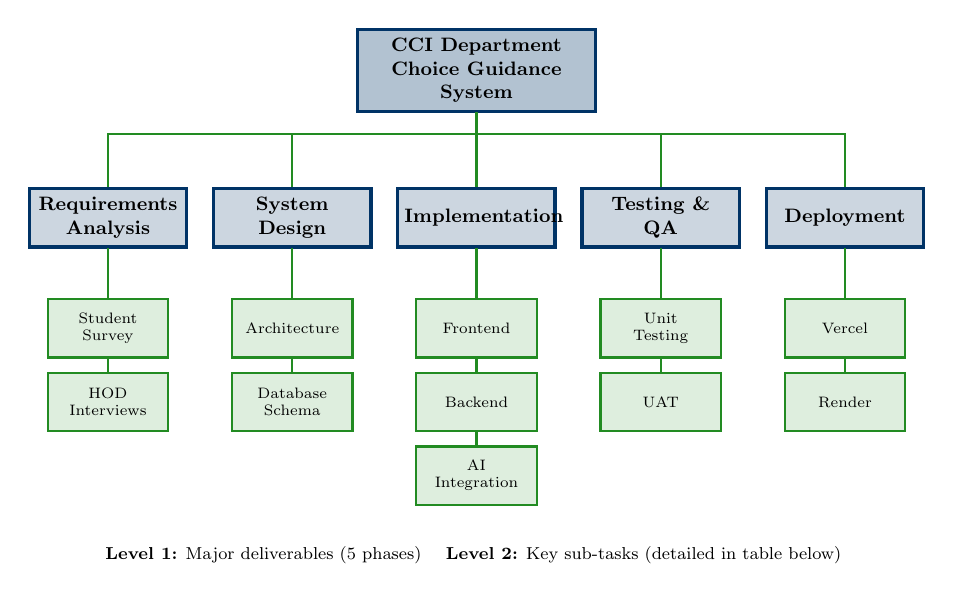
\begin{tikzpicture}[
    scale=0.78,
    transform shape,
    rootnode/.style={rectangle, draw=uniblue, very thick, fill=uniblue!30, text width=3.6cm, align=center, minimum height=1.05cm, inner sep=4pt, font=\bfseries\small},
    level1/.style={rectangle, draw=uniblue, very thick, fill=uniblue!20, text width=2.35cm, align=center, minimum height=0.95cm, inner sep=3pt, font=\small\bfseries},
    level2/.style={rectangle, draw=unigreen, thick, fill=unigreen!15, text width=1.75cm, align=center, minimum height=0.95cm, inner sep=3pt, font=\scriptsize},
    branch/.style={draw=unigreen, thick}
]

% Root node
\node[rootnode] (root) at (0, 0) {CCI Department\\Choice Guidance\\System};

% Level 1 - Main phases
\node[level1] (req)    at (-6, -2.4) {Requirements\\Analysis};
\node[level1] (design) at (-3, -2.4) {System\\Design};
\node[level1] (impl)   at (0,  -2.4) {Implementation};
\node[level1] (test)   at (3,  -2.4) {Testing \&\\QA};
\node[level1] (deploy) at (6,  -2.4) {Deployment};

% Root to phases
\draw[branch] (root.south) -- ++(0,-0.35) -| (req.north);
\draw[branch] (root.south) -- ++(0,-0.35) -| (design.north);
\draw[branch] (root.south) -- ++(0,-0.35) -- (0,-1.8) -- (impl.north);
\draw[branch] (root.south) -- ++(0,-0.35) -| (test.north);
\draw[branch] (root.south) -- ++(0,-0.35) -| (deploy.north);

% Level 2 - vertical branches beneath each phase
\node[level2] (req1)   at (-6, -4.2) {Student\\Survey};
\node[level2] (req2)   at (-6, -5.4) {HOD\\Interviews};
\draw[branch] (req.south) -- (req1.north);
\draw[branch] (req1.south) -- (req2.north);

\node[level2] (des1)   at (-3, -4.2) {Architecture};
\node[level2] (des2)   at (-3, -5.4) {Database\\Schema};
\draw[branch] (design.south) -- (des1.north);
\draw[branch] (des1.south) -- (des2.north);

\node[level2] (impl1)  at (0, -4.2) {Frontend};
\node[level2] (impl2)  at (0, -5.4) {Backend};
\node[level2] (impl3)  at (0, -6.6) {AI\\Integration};
\draw[branch] (impl.south) -- (impl1.north);
\draw[branch] (impl1.south) -- (impl2.north);
\draw[branch] (impl2.south) -- (impl3.north);

\node[level2] (test1)  at (3, -4.2) {Unit\\Testing};
\node[level2] (test2)  at (3, -5.4) {UAT};
\draw[branch] (test.south) -- (test1.north);
\draw[branch] (test1.south) -- (test2.north);

\node[level2] (dep1)   at (6, -4.2) {Vercel};
\node[level2] (dep2)   at (6, -5.4) {Render};
\draw[branch] (deploy.south) -- (dep1.north);
\draw[branch] (dep1.south) -- (dep2.north);

% Legend
\node[font=\footnotesize, align=center] at (0,-7.9) {
    \textbf{Level 1:} Major deliverables (5 phases) \quad \textbf{Level 2:} Key sub-tasks (detailed in table below)
};

\end{tikzpicture}
\caption{Work breakdown structure --- hierarchical task decomposition}
\label{fig:wbs-diagram}
\end{figure}

\subsubsection*{Level 1: Major Deliverables}

\begin{enumerate}[leftmargin=1.5em, itemsep=3pt]
    \item Project Management \& Planning
    \item Requirements Analysis \& Documentation
    \item System Design
    \item Frontend Development
    \item Backend Development
    \item AI Integration
    \item Testing \& Quality Assurance
    \item Deployment \& Operations
    \item Documentation \& Training
\end{enumerate}

\subsubsection*{Level 2: Detailed Task Breakdown}

\begin{table}[H]
\centering
\footnotesize
\begin{tabularx}{\textwidth}{>{\raggedright\arraybackslash}p{0.8cm}>{\raggedright\arraybackslash}p{3.5cm}>{\raggedright\arraybackslash}X>{\raggedright\arraybackslash}p{2.5cm}}
\toprule
\theadrow
\textbf{WBS ID} & \textbf{Task} & \textbf{Sub-tasks} & \textbf{Responsible} \\
\midrule
\textbf{1.0} & \textbf{Project Management} & & PM \\[2pt]
1.1 & Sprint Planning & Weekly sprint planning meetings, backlog grooming & Asledin \\[2pt]
1.2 & Daily Standups & 15-min daily coordination & All \\[2pt]
1.3 & Progress Tracking & Update GitHub Projects board, blockers resolution & Asledin \\[2pt]
1.4 & Stakeholder Communication & Weekly ICT Center updates, HOD coordination & Asledin \\[4pt]
\rowalt
\textbf{2.0} & \textbf{Requirements Analysis} & & PM + Team \\[2pt]
2.1 & Student Survey & Design, distribute, collect responses (n=43) & Nuri \\[2pt]
2.2 & HOD Interviews & Schedule, conduct, document 6 interviews & Asledin, Burqa \\[2pt]
2.3 & Survey Analysis & Quantitative stats, thematic analysis & Nuri \\[2pt]
2.4 & Requirements Doc & FR (12), NFR (13), use cases & All \\[4pt]
\textbf{3.0} & \textbf{System Design} & & Backend + PM \\[2pt]
3.1 & Architecture Design & 3-tier architecture, technology selection & Asledin \\[2pt]
3.2 & Database Schema & MongoDB collections, relationships & Asledin \\[2pt]
3.3 & API Design & REST endpoints, request/response formats & Asledin, Burqa \\[2pt]
3.4 & Data Flow Diagrams & Level 0, 1, 2 DFDs & Nuri \\[2pt]
3.5 & UI Wireframes & Assessment, results, comparison, admin pages & Arafat, Usman \\[4pt]
\rowalt
\textbf{4.0} & \textbf{Frontend Development} & & Frontend Team \\[2pt]
4.1 & React Setup & Project init, routing, state management & Arafat \\[2pt]
4.2 & Assessment UI & 20-question form, progress bar, validation & Usman \\[2pt]
4.3 & Results Page & Match scores, recommendations, explanations & Arafat \\[2pt]
4.4 & Comparison View & Side-by-side top 3 departments & Usman \\[2pt]
4.5 & Department Pages & 6 department profiles with curriculum & Arafat \\[2pt]
4.6 & Admin Dashboard & Login, content management, analytics & Usman \\[2pt]
4.7 & PDF Export & jsPDF integration, report generation & Usman \\[2pt]
4.8 & Responsive Design & Mobile-first CSS, cross-browser & Arafat \\[4pt]
\textbf{5.0} & \textbf{Backend Development} & & Backend Team \\[2pt]
5.1 & Express Server & Server setup, middleware, CORS & Asledin \\[2pt]
5.2 & MongoDB Integration & Mongoose schemas, connection & Asledin \\[2pt]
5.3 & Scoring Algorithm & Weighted calculation, normalization & Asledin \\[2pt]
5.4 & Authentication & JWT, bcrypt, admin login & Burqa \\[2pt]
5.5 & API Endpoints & Questions, departments, assessment, admin & Asledin, Burqa \\[2pt]
5.6 & Analytics Module & Usage tracking, aggregation & Burqa \\[4pt]
\rowalt
\textbf{6.0} & \textbf{AI Integration} & & Backend Team \\[2pt]
6.1 & OpenAI API Setup & API key, SDK configuration & Burqa \\[2pt]
6.2 & Prompt Engineering & Templates, context construction & Burqa \\[2pt]
6.3 & Timeout Handling & 5-second limit, fallback logic & Burqa \\[2pt]
6.4 & Response Parsing & Extract explanation from LLM output & Burqa \\[4pt]
\textbf{7.0} & \textbf{Testing \& QA} & & QA Lead \\[2pt]
7.1 & Unit Testing & Scoring algorithm, API endpoints & Nuri \\[2pt]
7.2 & Integration Testing & Frontend-backend, LLM API & Nuri, All \\[2pt]
7.3 & UAT & 10 volunteer students, feedback collection & Nuri \\[2pt]
7.4 & Cross-Browser & Chrome, Firefox, Safari, Edge & Nuri \\[2pt]
7.5 & Mobile Testing & iOS, Android devices & All \\[2pt]
7.6 & Bug Tracking & GitHub Issues, priority assignment & Nuri \\[4pt]
\rowalt
\textbf{8.0} & \textbf{Deployment} & & Backend + PM \\[2pt]
8.1 & Vercel Deployment & Frontend build, environment vars & Arafat \\[2pt]
8.2 & Render Deployment & Backend container, config & Asledin \\[2pt]
8.3 & MongoDB Atlas & Production cluster, backup & Asledin \\[2pt]
8.4 & Domain Configuration & DNS, SSL certificates & Asledin \\[4pt]
\textbf{9.0} & \textbf{Documentation} & & All \\[2pt]
9.1 & User Guide & How to complete assessment & Nuri \\[2pt]
9.2 & Admin Manual & Content management, analytics & Burqa \\[2pt]
9.3 & Technical Docs & Architecture, API, deployment & Asledin \\[2pt]
9.4 & Internship Report & LaTeX document (this report) & All \\
\bottomrule
\end{tabularx}
\caption{Work breakdown structure with task ownership}
\end{table}

\subsubsection*{Critical Path}

The following tasks represent the critical path (longest dependent task chain):

\begin{enumerate}[leftmargin=1.5em, itemsep=2pt]
    \item Requirements Analysis (Week 1--2) $\rightarrow$
    \item Database Schema Design (Week 2) $\rightarrow$
    \item Backend API Development (Week 3) $\rightarrow$
    \item Frontend Development (Week 4) $\rightarrow$
    \item Frontend-Backend Integration (Week 5) $\rightarrow$
    \item User Acceptance Testing (Week 5) $\rightarrow$
    \item Production Deployment (Week 6)
\end{enumerate}

Any delay in critical path tasks would directly impact the final delivery date.

\clearpage

% ══════════════════════════════════════════════════════════════════════════════
%  CHAPTER 2: SYSTEM REQUIREMENTS
% ══════════════════════════════════════════════════════════════════════════════
\newpage
\section{System Requirements}

% ─────────────────────────────────────────────────────────────────────────────
\subsection{Introduction}
% ─────────────────────────────────────────────────────────────────────────────

This chapter presents a comprehensive analysis of the current department selection process at Haramaya University's College of Computing and Informatics (CCI), identifies its limitations, and specifies the functional and non-functional requirements for the proposed CCI Department Choice Guidance System. The requirements were gathered through multiple sources including a structured student survey ($n = 43$), department head consultations, existing system analysis, and ICT Center stakeholder meetings.

% ─────────────────────────────────────────────────────────────────────────────
\subsubsection{Existing System Overview}
% ─────────────────────────────────────────────────────────────────────────────

Currently, incoming CCI students at Haramaya University select their department of specialization through an informal, largely unstructured process that relies on limited institutional guidance and fragmented information sources.

\paragraph{Current Department Selection Process}

The existing process follows this general flow:

\begin{enumerate}[leftmargin=1.5em, itemsep=3pt]
    \item \textbf{Enrollment (Week 1)}: Students admitted to CCI attend a general orientation session covering university policies, academic regulations, and basic college structure
    
    \item \textbf{Department Introduction (Week 1--2)}: Brief overview sessions (1--2 hours per department) where HODs or faculty representatives present their departments' focus areas, often during large group sessions with 100+ students
    
    \item \textbf{Informal Information Gathering (Week 1--3)}: Students independently seek information through:
    \begin{itemize}[leftmargin=1.5em, itemsep=2pt]
        \item Conversations with senior students (primary source)
        \item University website department pages (limited detail)
        \item Peer recommendations and social media groups
        \item Personal assumptions based on department names
    \end{itemize}
    
    \item \textbf{Department Selection (Week 2--3)}: Students submit their department preference (typically first and second choice) via paper forms to the CCI Dean's office
    
    \item \textbf{Administrative Placement (Week 3--4)}: Dean's office processes requests; in cases of oversubscription to popular departments, placements may be adjusted based on entrance exam scores or availability
    
    \item \textbf{Final Registration}: Students register for courses within their assigned department
\end{enumerate}

\paragraph{Available Information Sources}

The following information resources currently exist but are fragmented and incomplete:

\begin{table}[H]
\centering
\small
\begin{tabularx}{\textwidth}{>{\raggedright\arraybackslash}p{3.5cm}>{\raggedright\arraybackslash}X>{\raggedright\arraybackslash}p{3cm}}
\toprule
\theadrow
\textbf{Information Source} & \textbf{Content Provided} & \textbf{Accessibility} \\
\midrule
HOD Orientation Sessions & Department philosophy, basic curriculum overview, career mentions & One-time, large group, limited Q\&A \\[4pt]
\rowalt
University Website & Department names, brief descriptions (2--3 sentences), contact info & Online, outdated (last update 2021) \\[4pt]
Department Brochures & Varies by department; some have printed materials, others do not & Physical copies only, limited availability \\[4pt]
\rowalt
Course Catalog (PDF) & List of courses by department, credit hours, prerequisites & Online PDF, 200+ pages, difficult to navigate \\[4pt]
Senior Students (Informal) & Personal experiences, subjective opinions, workload perceptions & Accessible but inconsistent, biased \\[4pt]
\rowalt
Academic Advisors & Available for consultation but often contacted after selection & Limited appointments, reactive not proactive \\[4pt]
\bottomrule
\end{tabularx}
\caption{Current information sources for department selection}
\end{table}

\paragraph{Characteristics of the Existing System}

The current department selection process exhibits the following characteristics:

\begin{itemize}[leftmargin=1.5em, itemsep=3pt]
    \item \textbf{Decentralized Information}: No single authoritative source; students must piece together information from multiple channels
    
    \item \textbf{Time-Constrained}: 2--3 week decision window provides limited time for thoughtful exploration and comparison
    
    \item \textbf{Passive Approach}: System assumes students will proactively seek information; no structured guidance framework
    
    \item \textbf{One-Size-Fits-All}: General orientation sessions do not address individual student interests, aptitudes, or career goals
    
    \item \textbf{Limited Comparative Analysis}: Difficult for students to systematically compare departments on key dimensions (curriculum focus, career outcomes, required skills)
    
    \item \textbf{No Decision Support}: No tools, questionnaires, or frameworks to help students match their profiles to department characteristics
    
    \item \textbf{Paper-Based Administration}: Department selection forms submitted physically; no digital tracking or analytics
    
    \item \textbf{Reactive Advising}: Academic advisors provide guidance only when students seek it out, typically after preliminary decisions made
\end{itemize}

\paragraph{Survey Evidence of Current System Usage}

The student survey ($n = 43$) revealed how students actually navigate the existing system:

\begin{table}[H]
\centering
\small
\begin{tabularx}{\textwidth}{>{\raggedright\arraybackslash}p{5cm}>{\raggedright\arraybackslash}p{2.5cm}>{\raggedright\arraybackslash}X}
\toprule
\theadrow
\textbf{Information Source Used} & \textbf{Percentage} & \textbf{Perceived Usefulness (1--5)} \\
\midrule
Senior students / peers & 86.0\% & 3.4 (somewhat useful) \\[3pt]
\rowalt
HOD orientation sessions & 72.1\% & 3.1 (somewhat useful) \\[3pt]
University website & 44.2\% & 2.3 (not very useful) \\[3pt]
\rowalt
Personal assumptions & 41.9\% & 2.1 (not very useful) \\[3pt]
Course catalog review & 34.9\% & 2.8 (somewhat useful) \\[3pt]
\rowalt
Academic advisor consultation & 16.3\% & 3.9 (useful) \\[3pt]
Department brochures & 11.6\% & 2.5 (not very useful) \\[3pt]
\bottomrule
\end{tabularx}
\caption{Information sources used and perceived usefulness (survey results)}
\end{table}

The data shows heavy reliance on informal peer advice (86.0\%) despite moderate usefulness rating (3.4/5), while the most useful source—academic advisors (3.9/5)—was consulted by only 16.3\% of students, indicating a mismatch between information quality and accessibility.

% ─────────────────────────────────────────────────────────────────────────────
\subsubsection{Drawbacks of Existing System}
% ─────────────────────────────────────────────────────────────────────────────

Analysis of the current department selection process reveals multiple significant drawbacks that negatively impact students, departments, and institutional effectiveness.

\paragraph{1. Information Overload and Fragmentation}

\textbf{Problem}: Students encounter scattered, inconsistent information across multiple sources without a centralized, structured repository.

\textbf{Evidence}:
\begin{itemize}[leftmargin=1.5em, itemsep=2pt]
    \item Survey respondents reported consulting an average of 3.8 different information sources
    \item 44.2\% found the university website "not very useful" due to outdated or minimal content
    \item No single source provides comprehensive department comparisons
\end{itemize}

\textbf{Impact}: Students experience decision fatigue and information paralysis, often defaulting to simplistic heuristics (e.g., "CS is the hardest," "IT is practical") rather than informed analysis.

\paragraph{2. Lack of Personalized Guidance}

\textbf{Problem}: The one-size-fits-all orientation approach fails to address individual student profiles, interests, aptitudes, and career aspirations.

\textbf{Evidence}:
\begin{itemize}[leftmargin=1.5em, itemsep=2pt]
    \item Zero students surveyed reported receiving personalized recommendations
    \item HOD sessions accommodate 100+ students simultaneously, precluding individual attention
    \item No assessment tools to help students understand their own learning preferences or problem-solving styles
\end{itemize}

\textbf{Impact}: Students with non-obvious fits (e.g., business-oriented CS students better suited for IS, theory-inclined IT students better suited for CS) remain unidentified.

\paragraph{3. Heavy Reliance on Peer Advice}

\textbf{Problem}: 86.0\% of students rely primarily on senior student opinions, which are inherently subjective, limited to individual experiences, and often perpetuate departmental stereotypes.

\textbf{Evidence}:
\begin{itemize}[leftmargin=1.5em, itemsep=2pt]
    \item Peer advice rated only 3.4/5 usefulness despite being most commonly used
    \item Senior students lack comprehensive knowledge of all six departments
    \item Advice often reflects personal biases ("I regret choosing X" or "Y is the best")
\end{itemize}

\textbf{Impact}: Perpetuation of myths ("Statistics is only for mathematicians," "ISC has no jobs"), unequal departmental visibility, and herd mentality toward perceived "popular" departments.

\paragraph{4. Inadequate Comparative Framework}

\textbf{Problem}: No structured method for students to systematically compare departments across key decision dimensions.

\textbf{Evidence}:
\begin{itemize}[leftmargin=1.5em, itemsep=2pt]
    \item No side-by-side comparison charts or matrices available
    \item Students reported difficulty understanding differences between similar-sounding departments (IS vs. ISC, CS vs. SWE)
    \item Survey open-ended responses frequently requested "clear differentiation" and "comparative tables"
\end{itemize}

\textbf{Impact}: Students struggle to articulate why they chose their department beyond superficial reasons; difficulty distinguishing between similar programs leads to mismatches.

\paragraph{5. Time Pressure and Rushed Decisions}

\textbf{Problem}: 2--3 week decision window is insufficient for thoughtful exploration, especially for students unfamiliar with computing disciplines.

\textbf{Evidence}:
\begin{itemize}[leftmargin=1.5em, itemsep=2pt]
    \item 67.4\% of survey respondents felt the decision timeline was "too short"
    \item Students must simultaneously adapt to university life, attend orientation events, and make a career-shaping decision
    \item No mechanisms for students to revisit or revise preliminary thinking
\end{itemize}

\textbf{Impact}: Hasty decisions based on incomplete information; regret and transfer requests in subsequent semesters.

\paragraph{6. No Decision Support Tools}

\textbf{Problem}: Absence of assessment questionnaires, recommendation algorithms, or decision aids that match student characteristics to department profiles.

\textbf{Evidence}:
\begin{itemize}[leftmargin=1.5em, itemsep=2pt]
    \item 97.7\% of students indicated they would use a recommendation tool if available
    \item No existing tools or frameworks beyond informal peer conversations
    \item Students expressed desire for "something like a quiz to tell me which department fits"
\end{itemize}

\textbf{Impact}: Students lack confidence in their choices; 44.2\% reported not feeling "fully confident" in understanding department differences when making their selection.

\paragraph{7. Unbalanced Enrollment Patterns}

\textbf{Problem}: Without objective guidance, students gravitate toward departments with higher perceived prestige or familiarity, leading to overcrowding and resource strain.

\textbf{Evidence}:
\begin{itemize}[leftmargin=1.5em, itemsep=2pt]
    \item Computer Science and Software Engineering consistently oversubscribed
    \item Information Science and Statistics receive fewer first-choice selections despite strong career prospects
    \item Administrative burden of managing transfer requests between departments
\end{itemize}

\textbf{Impact}: Inefficient resource utilization; some departments operate near capacity while others are underutilized; qualified students placed in non-preferred departments due to quotas.

\paragraph{8. Administrative Inefficiency}

\textbf{Problem}: Paper-based selection process lacks analytics, tracking, or data-driven insights for enrollment planning.

\textbf{Evidence}:
\begin{itemize}[leftmargin=1.5em, itemsep=2pt]
    \item No aggregated data on student interest trends, decision factors, or satisfaction patterns
    \item Manual processing of paper forms creates administrative burden
    \item No visibility into "runner-up" preferences (students' second/third choices)
\end{itemize}

\textbf{Impact}: Departments cannot anticipate enrollment trends; missed opportunities for data-informed curriculum development and marketing.

\paragraph{Summary of Drawbacks}

\begin{table}[H]
\centering
\small
\begin{tabularx}{\textwidth}{>{\raggedright\arraybackslash}p{1cm}>{\raggedright\arraybackslash}p{4cm}>{\raggedright\arraybackslash}X}
\toprule
\theadrow
\textbf{No.} & \textbf{Drawback} & \textbf{Primary Consequence} \\
\midrule
1 & Information fragmentation & Decision fatigue, incomplete understanding \\[3pt]
\rowalt
2 & No personalized guidance & Mismatched placements, unidentified fits \\[3pt]
3 & Over-reliance on peer advice & Perpetuation of myths, biased perspectives \\[3pt]
\rowalt
4 & Lack of comparison framework & Difficulty distinguishing similar departments \\[3pt]
5 & Rushed decision timeline & Hasty choices, post-decision regret \\[3pt]
\rowalt
6 & No decision support tools & Low confidence, uninformed selections \\[3pt]
7 & Unbalanced enrollment & Resource inefficiency, quota-based rejections \\[3pt]
\rowalt
8 & Paper-based administration & No analytics, missed planning opportunities \\[3pt]
\bottomrule
\end{tabularx}
\caption{Summary of existing system drawbacks and consequences}
\end{table}

These drawbacks collectively create a suboptimal decision environment that fails to serve the best interests of students, departments, or the institution, providing strong justification for the development of the CCI Department Choice Guidance System.

\clearpage

% ══════════════════════════════════════════════════════════════════════════════
%  CHAPTER 3: REQUIREMENTS ANALYSIS
% ══════════════════════════════════════════════════════════════════════════════
\newpage
\section{Requirements Analysis}

\subsection{System models}
System modeling is essential for visualizing the interaction between users and the system. It helps in understanding the flow of data and the behavior of the system under different conditions. 

\subsubsection{Scenarios}
Scenarios help define how users interact with the system in real-world situations:

\begin{itemize}
    \item \textbf{Student Assessment Scenario}: A freshman student visits the application, enters their basic information, and begins the 20-question interactive assessment. The system processes the answers in real-time, calculates the department compatibility scores, and displays the top recommended departments along with detailed career paths for each.
    
    \item \textbf{Administrator Management Scenario}: An administrator logs into the system dashboard to view aggregate student assessment data. They use the dashboard to identify popular department trends and update existing questions or department information to ensure the guidance provided remains current and relevant.
\end{itemize}

\subsubsection{Use case model}
The use case model illustrates the functional requirements of the system by identifying the actors and their interactions. This model serves as a high-level representation, capturing the exchanges between external actors (Students and Administrators) and the system boundaries. It provides a structured view of the services provided by the system, ensuring that all necessary functionalities—from student assessment to administrative data management—are clearly identified and aligned with stakeholder needs. By defining these use cases, we establish a formal mapping between the system's capabilities and user expectations, which serves as a blueprint for subsequent development phases.

\begin{figure}[H]
    \centering
    % [Insert Use Case Diagram here]
    \caption{Use Case Diagram}
    \label{fig:use_case}
\end{figure}

\begin{itemize}
    \item \textbf{Actors}: 
    \begin{itemize}
        \item \textbf{Student}: The primary user who interacts with the assessment system.
        \item \textbf{Administrator}: Manages the content of the system, including questions and department details.
    \end{itemize}
    \item \textbf{Main Use Cases}:
    \begin{itemize}
        \item \textbf{Take Assessment}: Student completes the 20-question survey.
        \item \textbf{View Results}: Student sees personalized department recommendations.
        \item \textbf{Compare Departments}: Student performs side-by-side analysis of CCI departments.
        \item \textbf{Manage Content}: Administrator updates questions and department metadata.
        \item \textbf{View Analytics}: Administrator analyzes aggregated student preference data.
    \end{itemize}
\end{itemize}

\subsubsection{Object model (Class and Object diagrams)}
The object model defines the static structure of the system, representing the entities and their relationships:

\begin{figure}[H]
    \centering
    % [Insert Class Diagram here]
    \caption{Class Diagram}
    \label{fig:class_diagram}
\end{figure}

\begin{figure}[H]
    \centering
    % [Insert Object Diagram here]
    \caption{Object Diagram}
    \label{fig:object_diagram}
\end{figure}

\begin{itemize}
    \item \textbf{Core Classes}:
    \begin{itemize}
        \item \textbf{User}: Represents the student or administrator.
        \item \textbf{Department}: Holds information about the various CCI departments.
        \item \textbf{Question}: Represents individual assessment inquiries.
        \item \textbf{Assessment}: Captures the user's responses and calculated scores.
    \end{itemize}
    \item \textbf{Relationships}: The \textbf{Assessment} class aggregates multiple \textbf{Question} responses, while the \textbf{Department} class holds associated \textbf{CareerPath} and \textbf{FocusArea} information.
\end{itemize}

\subsubsection{Dynamic model (Sequence, Activity, state Chart Diagrams)}
The dynamic model describes the system's behavior over time:

The dynamic model describes the system's behavior over time through various diagrams:

\begin{itemize}
    \item \textbf{Sequence Diagram}: This diagram visualizes the interaction between system components over time. Specifically, it models the flow of data when a student submits an assessment: the User Interface captures input, sends it to the Controller, which invokes the Scoring Logic, and finally returns the result to the Results View. It highlights the order of operations and message exchanges within the system.

\begin{figure}[H]
    \centering
    % [Insert Sequence Diagram here]
    \caption{Sequence Diagram}
    \label{fig:sequence_diagram}
\end{figure}

    \item \textbf{Activity Diagram}: This diagram maps the procedural flow of the assessment process. It illustrates the step-by-step logic from the initiation of the survey, through the sequential processing of questions, to the final generation and display of department recommendations, providing a clear overview of the assessment workflow.

\begin{figure}[H]
    \centering
    % [Insert Activity Diagram here]
    \caption{Activity Diagram}
    \label{fig:activity_diagram}
\end{figure}

    \item \textbf{State Chart Diagram}: This diagram defines the lifecycle and transitions of an assessment entity. It captures the states an assessment can exist in, such as \textit{Not Started}, \textit{In Progress}, and \textit{Completed}, along with the conditions or triggers that cause the transition from one state to another, ensuring the integrity of the assessment process.

\begin{figure}[H]
    \centering
    % [Insert State Chart Diagram here]
    \caption{State Chart Diagram}
    \label{fig:state_chart}
\end{figure}
\end{itemize}

\subsubsection{User interface—navigational paths and screen mock-ups}
The user interface is designed with a user-centered approach, prioritizing simplicity, accessibility, and responsiveness across all devices. The design philosophy aims to minimize cognitive load, allowing students to navigate the assessment and view results with minimal friction.

\begin{figure}[H]
    \centering
    % [Insert Screen Mock-ups here]
    \caption{Screen Mock-ups}
    \label{fig:screen_mockups}
\end{figure}

\begin{itemize}
    \item \textbf{Navigational Path}: 
    The navigation follows a linear, intuitive flow:
    \begin{itemize}
        \item \textbf{Home}: Entry point providing project context.
        \item \textbf{Assessment Interface}: Progressive sequence of screens for capturing user data.
        \item \textbf{Results/Comparison Dashboard}: Final landing page for insights and recommendations.
    \end{itemize}

    \item \textbf{Screens Detail}:
    \begin{itemize}
        \item \textbf{Welcome Screen}: Features a clean, welcoming layout with a prominent call-to-action to begin the assessment, ensuring students immediately understand the purpose of the platform.
        \item \textbf{Assessment Interface}: Employs a focus-mode design, displaying one question at a time to minimize distraction and ensure accurate user responses.
        \item \textbf{Results/Comparison Panel}: Utilizes a combination of intuitive visual cards for high-level summaries and interactive tables for a detailed, side-by-side comparison of departmental focus areas and career paths.
        \item \textbf{Admin Dashboard}: A secure, data-rich interface providing administrators with actionable insights into student trends, question performance, and overall system engagement.
    \end{itemize}
\end{itemize}

\subsection{Glossary}
\begin{description}
    \item[CCI] College of Computing and Informatics at Haramaya University.
    \item[Assessment] An interactive survey used to evaluate student interests and skills.
    \item[Recommendation] A personalized department suggestion based on calculated compatibility scores.
    \item[Administrator] A user with privileges to manage application content, such as questions and department data.
    \item[Compatibility Score] A quantitative measure indicating how well a student's profile aligns with a specific department.
\end{description}

% ══════════════════════════════════════════════════════════════════════════════
%  CHAPTER 4: SYSTEM DESIGN
% ══════════════════════════════════════════════════════════════════════════════
\newpage
\section{System Design}

\subsection{Introduction}
This chapter details the design principles, architectural choices, and the structured development process followed during the implementation of the application. It serves as a bridge between the requirements gathered in the previous chapter and the actual technical execution, outlining how the system's modular components are designed to work together to satisfy the identified needs.

\subsubsection{Overview of System Design}
The system design process translates the functional and non-functional requirements into a concrete technical specification. It defines the structural and behavioral blueprints necessary for development, ensuring that the final implementation is robust, scalable, and fully aligned with the intended user experience.

\subsubsection{Design Goal}
The primary design goal is to create a seamless, intuitive, and efficient platform that accurately matches students with their ideal departments based on their unique profiles. Key objectives include ensuring system responsiveness, maintaining data integrity, providing clear and actionable recommendations, and adhering to maintainable coding practices for future enhancements.

\subsection{Current Software Architecture}
The system architecture follows a modular, client-server approach designed for performance, scalability, and maintainability. It is structured into three primary layers:

\begin{itemize}
    \item \textbf{Frontend Layer}: Built with React.js, responsible for the user interface, assessment interaction, and real-time visualization of results.
    \item \textbf{API Layer}: A Node.js and Express.js server acting as the bridge between the frontend and database, handling authentication, data validation, and business logic.
    \item \textbf{Data Layer}: A MongoDB Atlas NoSQL database providing flexible storage for department content, questions, and session-based assessment responses.
\end{itemize}

\subsection{Proposed Software Architecture}

\subsubsection{Overview}
The proposed architecture builds upon the current modular framework by introducing enhanced scalability features and improved integration patterns. Key improvements include the adoption of an asynchronous event-driven design to better handle high-concurrency requests during peak assessment periods and the implementation of advanced caching strategies to optimize recommendation generation speeds. This architecture ensures long-term system stability and flexibility for integrating additional AI-driven analytical tools.

\subsubsection{Sub-system Decomposition with Services (with Deployment Diagram)}
To promote scalability and maintainability, the system is decomposed into distinct, loosely coupled services. The core sub-systems include the User Interface (Frontend Dashboard and Assessment Module), the Core API Services (Authentication, Matching Engine, and Assessment Manager), and the Data Persistence Layer. The deployment diagram below illustrates how these services are distributed and orchestrated across the cloud infrastructure.

\begin{figure}[H]
    \centering
    % \includegraphics[width=0.85\textwidth]{figures/deployment_diagram.png}
    \vspace{4cm} % Placeholder space for the diagram
    \caption{Deployment Diagram of the Proposed Architecture}
    \label{fig:deployment_diagram}
\end{figure}

\subsubsection{Hardware / Software mapping}
The hardware/software mapping defines how the software components of the system are deployed onto the underlying physical and virtual infrastructure. 

\begin{itemize}[leftmargin=1.5em, itemsep=3pt]
    \item \textbf{Client Devices (Hardware)}: User devices such as laptops, desktops, and smartphones run standard web browsers (Software) to access the Frontend User Interface.
    \item \textbf{Application Servers (Virtual Hardware)}: Cloud-based virtual machines or serverless containers host the backend API services, matching engine, and routing logic.
    \item \textbf{Database Servers (Hardware/Cluster)}: A dedicated cloud cluster (e.g., MongoDB Atlas) hosts the NoSQL database management system, ensuring high availability, data persistence, and secure backups.
\end{itemize}
This mapping ensures that resource-intensive operations are executed on scalable cloud servers, providing a smooth and responsive experience on the end user's local device.

\subsubsection{Database design}
The database architecture is designed to prioritize data integrity, scalability, and fast read/write operations. At a conceptual level, it is structured around the core workflow of the application: a user taking an assessment to receive a department recommendation.

\textbf{Conceptual Model \& Entities} \\
The data is logically organized into several key entities:
\begin{itemize}[leftmargin=1.5em, itemsep=3pt]
    \item \textbf{Users}: Stores authentication credentials, profile information, and role-based access levels.
    \item \textbf{Departments}: Contains the profiles for each department, including skill requirements and matching criteria.
    \item \textbf{Assessments}: Holds the pool of questions, potential answers, and associated skill weightings.
    \item \textbf{Results}: Records submitted student responses, generated profile metrics, and recommendation outcomes.
\end{itemize}

These entities interact through specific relational mappings: a single \textit{User} can generate multiple \textit{Results} (1:N), many \textit{Results} map to a single \textit{Department} (N:1), and \textit{Users} interact with various \textit{Assessments} mapped to multiple \textit{Departments} (N:M). 

To visualize these relationships, an Entity-Relationship (ER) diagram is provided below, illustrating the cardinalities and logical connections between the primary entities.

\begin{figure}[H]
    \centering
    % \includegraphics[width=0.85\textwidth]{figures/er_diagram.png}
    \vspace{4cm} % Placeholder space for the diagram
    \caption{Entity-Relationship (ER) Diagram of the Database}
    \label{fig:er_diagram}
\end{figure}

To maintain rigorous standards for data quality and system reliability, the database design adheres to the following core architectural principles:

\vspace{0.5em}
\noindent\textbf{\checkmark Normalization: no less than 2nd normal form} \\
The database schema is strictly normalized to \textbf{no less than the 2nd Normal Form (2NF)}. This ensures that redundant data is eliminated and that all non-key attributes are fully functionally dependent on the primary key, thereby preventing update, insertion, and deletion anomalies.

To illustrate this normalized structure, Table \ref{tab:db_schema_example} provides an example schema for the \textbf{Users}, \textbf{Departments}, and \textbf{Results} entities, demonstrating the clear separation of data and the use of primary and foreign keys to define relationships.

\begin{table}[H]
    \centering
    \caption{Example of Normalized Database Schema (2NF compliant)}
    \label{tab:db_schema_example}
    \begin{tabular}{llp{3cm}p{6cm}}
        \toprule
        \textbf{Entity} & \textbf{Attribute} & \textbf{Data Type} & \textbf{Constraints} \\ 
        \midrule
        \textbf{Users} 
        & UserID & INT & Primary Key, Auto-increment \\
        & FullName & VARCHAR(100) & Not Null \\
        & Email & VARCHAR(100) & Unique, Not Null \\
        & Role & VARCHAR(50) & Default 'Student' \\ 
        \midrule
        \textbf{Departments}
        & DeptID & INT & Primary Key, Auto-increment \\
        & DeptName & VARCHAR(100) & Not Null \\
        & RequiredScore & DECIMAL(5,2) & Not Null \\
        \midrule
        \textbf{Results} 
        & ResultID & INT & Primary Key, Auto-increment \\
        & UserID & INT & Foreign Key (References Users.UserID) \\
        & DepartmentID & INT & Foreign Key (References Departments.DeptID) \\
        & MatchScore & DECIMAL(5,2) & Not Null \\
        & DateSubmitted & TIMESTAMP & Default CURRENT\_TIMESTAMP \\ 
        \bottomrule
    \end{tabular}
\end{table}

\vspace{0.5em}
\noindent\textbf{\checkmark Persistent Data management} \\
The system employs robust persistent data management strategies. All critical records—such as user credentials, submitted assessments, and calculated recommendations—are written to durable storage. This guarantees high availability, enables routine backups, and ensures that data remains intact and recoverable across system restarts, network interruptions, or unexpected hardware failures. 

A critical aspect of this persistence is the management of active session data. As a user progresses through an assessment, their intermediate responses are continuously synchronized with the database. This reliable state-saving mechanism allows users to safely pause and resume unfinished assessments at a later time, even across different devices, without the risk of losing their progress or having to restart the evaluation.

\subsubsection{Access Control and Security}
To safeguard user data and maintain the integrity of the assessment platform, robust security measures and strict access control policies are implemented throughout the architecture.

\begin{itemize}[leftmargin=1.5em, itemsep=3pt]
    \item \textbf{Role-Based Access Control (RBAC)}: The system defines distinct user roles to restrict access to sensitive functionalities. \textit{Students} are granted access only to the assessment interface and their personal recommendation results. \textit{Administrators} are provided with privileged access to manage department criteria, update assessment questions, and view aggregate analytical data.
    \item \textbf{Authentication and Authorization}: Secure authentication protocols (such as JSON Web Tokens) are employed to verify user identities. Every API request is validated against authorization tokens to ensure the requester has the appropriate permissions.
    \item \textbf{Data Encryption}: To protect data against unauthorized interception, all data transmitted between the client interface and the backend API is encrypted in transit using TLS/SSL protocols. Additionally, sensitive data stored within the database, such as user passwords, is securely hashed and salted using industry-standard cryptographic algorithms.
\end{itemize}

\subsubsection{Global control flow}
The global control flow dictates the sequence of operations and the interactions between subsystems from the moment a user initiates a session until the final recommendation is delivered.

\begin{enumerate}[leftmargin=1.5em, itemsep=3pt]
    \item \textbf{Initialization}: The user accesses the frontend interface and authenticates. The system validates the credentials and establishes a secure session using JWTs.
    \item \textbf{Assessment Execution}: The frontend retrieves the assessment questions from the API layer and presents them to the user. As the user progresses, responses are captured and held in the frontend state manager.
    \item \textbf{Data Submission and Processing}: Upon completion, the frontend packages the responses and submits them to the backend API. The API validates the payload and forwards it to the Matching Engine.
    \item \textbf{Matching and Recommendation}: The Matching Engine queries the database to retrieve department profiles and criteria. It executes the scoring algorithm against the user's submitted responses to calculate match percentages for each department.
    \item \textbf{Result Delivery}: The calculated results are written to the database for historical tracking, and the optimal department recommendations are returned as a structured response to the frontend.
    \item \textbf{Visualization}: The frontend renders the comparison dashboard, displaying personalized recommendations and analytical insights to the student.
\end{enumerate}

\subsubsection{Boundary Condition}
Boundary conditions define how the system behaves during edge cases, unexpected failures, initialization, and termination, ensuring high reliability and fault tolerance.

\begin{itemize}[leftmargin=1.5em, itemsep=3pt]
    \item \textbf{System Initialization and Recovery}: In the event of a system restart or crash, services are designed to automatically reconnect to the database. Uncompleted assessments stored in the frontend's local storage can be resumed by the user, preventing data loss.
    \item \textbf{Network Interruptions}: If a user loses internet connection during the assessment, the frontend gracefully degrades, alerting the user and caching responses locally until the connection is restored and payload submission can be retried.
    \item \textbf{Edge Cases in Matching}: The matching engine is programmed to handle algorithmic ties (e.g., when a student scores exactly the same percentage for two distinct departments) by recommending both paths equally alongside comparative insights.
    \item \textbf{Data Validation}: The API layer implements strict payload validation. Any incomplete assessments or malformed requests are rejected with clear error codes, preventing corruption of the recommendation engine or database structure.
\end{itemize}

% ─────────────────────────────────────────────────────────────────────────────
\subsection{Subsystem services}
% ─────────────────────────────────────────────────────────────────────────────

The architecture is composed of several independent, highly cohesive subsystem services that interact to deliver the complete functionality of the platform. These services are categorized into Frontend, Backend API, and Data Persistence layers.

\subsubsection{Frontend Services (Client-Side)}
The frontend subsystem operates on the user's device and is responsible for rendering the interface and managing local application state.
\begin{itemize}[leftmargin=1.5em, itemsep=3pt]
    \item \textbf{Authentication UI Service}: Manages user login, registration, and session token storage. It communicates directly with the backend to securely authenticate users before granting access to the main application.
    \item \textbf{Assessment Interface Service}: Dynamically renders the assessment questions, captures real-time user inputs, and temporarily caches session data locally to prevent data loss during network interruptions.
    \item \textbf{Dashboard \& Visualization Service}: Consumes the calculated recommendation data from the backend and renders interactive charts and comparative insights, allowing students to visually explore their optimal department matches.
\end{itemize}

\subsubsection{Backend API Services (Server-Side)}
The backend subsystem serves as the core processing engine of the application, exposing secure RESTful endpoints for the frontend to consume.
\begin{itemize}[leftmargin=1.5em, itemsep=3pt]
    \item \textbf{User Management Service}: Handles secure password hashing, JWT token generation, and role-based authorization checks for all incoming requests.
    \item \textbf{Assessment Manager}: Retrieves the latest question banks from the database and validates incoming assessment payloads submitted by the frontend.
    \item \textbf{Matching Engine Service}: The analytical core of the platform. It executes the proprietary scoring algorithm, comparing user assessment responses against department criteria to generate match percentage scores.
\end{itemize}

\subsubsection{Data Persistence Services}
The data persistence layer abstracts the physical database operations away from the core business logic.
\begin{itemize}[leftmargin=1.5em, itemsep=3pt]
    \item \textbf{Profile Storage Service}: Manages the CRUD (Create, Read, Update, Delete) operations for User and Department entities, ensuring 2NF normalization and referential integrity.
    \item \textbf{Recommendation Logging Service}: Securely writes the generated match results and historical assessment data to durable storage for future retrieval and administrative analytics.
\end{itemize}

% ─────────────────────────────────────────────────────────────────────────────
\subsection{Data dictionary}
% ─────────────────────────────────────────────────────────────────────────────

A Data Dictionary provides a detailed description of the data elements, their types, constraints, and relationships within the system's database schema. It serves as a central reference to ensure consistency and a clear understanding of the persistent data architecture. The following tables outline the definitions for the primary entities.

\begin{table}[H]
    \centering
    \caption{Data Dictionary: Users Entity}
    \label{tab:dd_users}
    \begin{tabular}{lp{2cm}p{3cm}p{6cm}}
        \toprule
        \textbf{Attribute Name} & \textbf{Data Type} & \textbf{Constraints} & \textbf{Description} \\ 
        \midrule
        UserID & INT & PK, Auto-inc & Unique identifier for each user. \\
        FullName & VARCHAR(100) & Not Null & The user's complete legal name. \\
        Email & VARCHAR(100) & Unique, Not Null & Contact email, used for authentication. \\
        PasswordHash & VARCHAR(255) & Not Null & Securely hashed string of the user's password. \\
        Role & VARCHAR(50) & Default 'Student' & Defines RBAC privileges (e.g., Student, Admin). \\ 
        CreatedAt & TIMESTAMP & Default NOW() & Timestamp indicating when the account was created. \\
        \bottomrule
    \end{tabular}
\end{table}

\begin{table}[H]
    \centering
    \caption{Data Dictionary: Departments Entity}
    \label{tab:dd_departments}
    \begin{tabular}{lp{2cm}p{3cm}p{6cm}}
        \toprule
        \textbf{Attribute Name} & \textbf{Data Type} & \textbf{Constraints} & \textbf{Description} \\ 
        \midrule
        DeptID & INT & PK, Auto-inc & Unique identifier for each department. \\
        DeptName & VARCHAR(100) & Not Null & Name of the academic or organizational department. \\
        Description & TEXT & Nullable & Detailed overview of the department's focus. \\
        RequiredScore & DECIMAL(5,2) & Not Null & The minimum threshold score required for a match. \\
        \bottomrule
    \end{tabular}
\end{table}

\begin{table}[H]
    \centering
    \caption{Data Dictionary: Results Entity}
    \label{tab:dd_results}
    \begin{tabular}{lp{2cm}p{3cm}p{6cm}}
        \toprule
        \textbf{Attribute Name} & \textbf{Data Type} & \textbf{Constraints} & \textbf{Description} \\ 
        \midrule
        ResultID & INT & PK, Auto-inc & Unique identifier for the assessment result record. \\
        UserID & INT & FK $\rightarrow$ Users & Identifies which user completed the assessment. \\
        DepartmentID & INT & FK $\rightarrow$ Depts & Identifies the recommended department. \\
        MatchScore & DECIMAL(5,2) & Not Null & The calculated percentage match (e.g., 85.50). \\
        DateSubmitted & TIMESTAMP & Default NOW() & Timestamp indicating when the result was computed. \\ 
        \bottomrule
    \end{tabular}
\end{table}

% ─────────────────────────────────────────────────────────────────────────────
\subsection{Glossary}
% ─────────────────────────────────────────────────────────────────────────────

A glossary of key technical terms and acronyms used throughout this architectural design document to ensure clarity:

\begin{description}[leftmargin=1.5em, itemsep=4pt, font=\textbf]
    \item[API (Application Programming Interface)] A set of protocols and tools that allows different software applications to communicate and share data with one another.
    \item[CRUD] An acronym for Create, Read, Update, and Delete, representing the four fundamental operations of persistent database storage.
    \item[ER Diagram (Entity-Relationship Diagram)] A visual model used in database design to illustrate the logical structure of data entities and their relational dependencies.
    \item[JWT (JSON Web Token)] A compact, URL-safe token format commonly used for authenticating users and securely transmitting information between parties.
    \item[Normalization (2NF)] The process of structuring a relational database to reduce data redundancy. Second Normal Form (2NF) ensures that all non-key attributes are fully functionally dependent on the primary key.
    \item[RBAC (Role-Based Access Control)] A security management framework that restricts system access and operational privileges based on the assigned roles of individual users (e.g., Student vs. Administrator).
    \item[TLS/SSL] Cryptographic protocols designed to provide communications security over a computer network, ensuring data encrypted in transit remains private.
\end{description}

% ─────────────────────────────────────────────────────────────────────────────
\subsection{Project Schedule}
% ─────────────────────────────────────────────────────────────────────────────

The project follows a 6-week development timeline. The Gantt chart below visualizes phases, their durations, and the current status marker.

\begin{figure}[H]
\centering
\resizebox{\textwidth}{!}{%
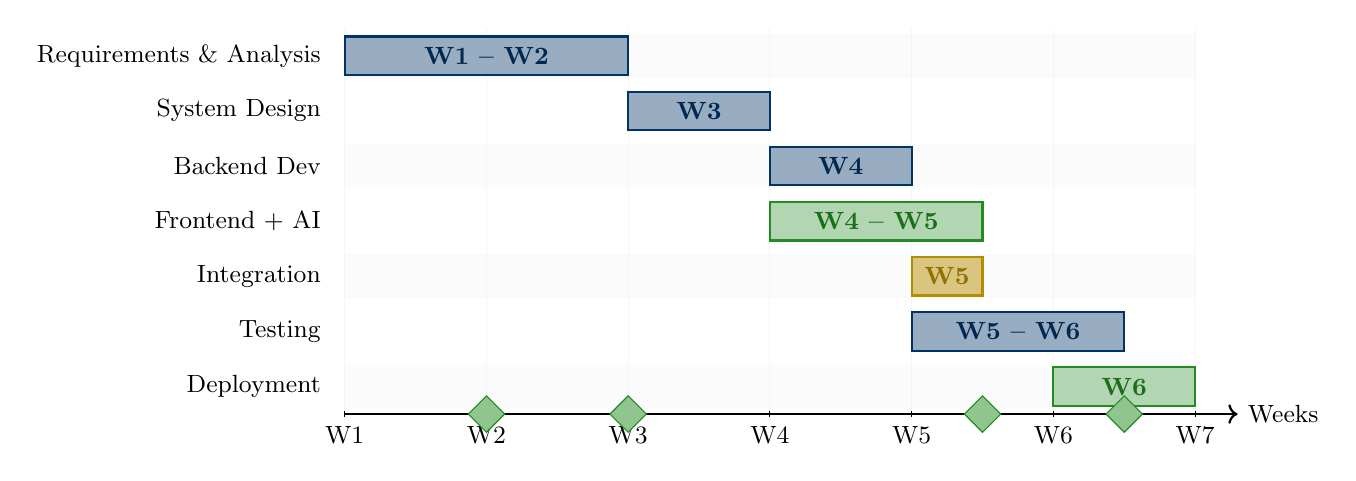
\begin{tikzpicture}[x=1.8cm, y=0.7cm]
\node[anchor=east, font=\small] at (0.9, 7) {Requirements \& Analysis};
\node[anchor=east, font=\small] at (0.9, 6) {System Design};
\node[anchor=east, font=\small] at (0.9, 5) {Backend Dev};
\node[anchor=east, font=\small] at (0.9, 4) {Frontend + AI};
\node[anchor=east, font=\small] at (0.9, 3) {Integration};
\node[anchor=east, font=\small] at (0.9, 2) {Testing};
\node[anchor=east, font=\small] at (0.9, 1) {Deployment};
\fill[lightgray!40] (1,6.6) rectangle (7,7.4);
\fill[lightgray!40] (1,4.6) rectangle (7,5.4);
\fill[lightgray!40] (1,2.6) rectangle (7,3.4);
\fill[lightgray!40] (1,0.6) rectangle (7,1.4);
\foreach \x in {1,2,...,7}
    \draw[lightgray, thin] (\x,0.5) -- (\x,7.5);
\fill[uniblue!40] (1,6.65) rectangle (3,7.35); \draw[uniblue,thick] (1,6.65) rectangle (3,7.35);
\node[font=\small\bfseries, text=uniblue!80!black] at (2,7) {W1 -- W2};
\fill[uniblue!40] (3,5.65) rectangle (4,6.35); \draw[uniblue,thick] (3,5.65) rectangle (4,6.35);
\node[font=\small\bfseries, text=uniblue!80!black] at (3.5,6) {W3};
\fill[uniblue!40] (4,4.65) rectangle (5,5.35); \draw[uniblue,thick] (4,4.65) rectangle (5,5.35);
\node[font=\small\bfseries, text=uniblue!80!black] at (4.5,5) {W4};
\fill[unigreen!35] (4,3.65) rectangle (5.5,4.35); \draw[unigreen,thick] (4,3.65) rectangle (5.5,4.35);
\node[font=\small\bfseries, text=unigreen!80!black] at (4.75,4) {W4 -- W5};
\fill[accentgold!50] (5,2.65) rectangle (5.5,3.35); \draw[accentgold,thick] (5,2.65) rectangle (5.5,3.35);
\node[font=\small\bfseries, text=accentgold!80!black] at (5.25,3) {W5};
\fill[uniblue!40] (5,1.65) rectangle (6.5,2.35); \draw[uniblue,thick] (5,1.65) rectangle (6.5,2.35);
\node[font=\small\bfseries, text=uniblue!80!black] at (5.75,2) {W5 -- W6};
\fill[unigreen!35] (6,0.65) rectangle (7,1.35); \draw[unigreen,thick] (6,0.65) rectangle (7,1.35);
\node[font=\small\bfseries, text=unigreen!80!black] at (6.5,1) {W6};

\draw[thick, ->] (1,0.5) -- (7.3,0.5) node[anchor=west, font=\small] {Weeks};
\foreach \x in {1,2,...,7}
    \draw (\x,0.55) -- (\x,0.45) node[anchor=north, font=\small] {W\x};
\node[diamond, draw=unigreen, fill=unigreen!50, minimum size=0.35cm] at (2,0.5) {};
\node[diamond, draw=unigreen, fill=unigreen!50, minimum size=0.35cm] at (3,0.5) {};
\node[diamond, draw=unigreen, fill=unigreen!50, minimum size=0.35cm] at (5.5,0.5) {};
\node[diamond, draw=unigreen, fill=unigreen!50, minimum size=0.35cm] at (6.5,0.5) {};
\end{tikzpicture}%
}
\caption{Project Gantt chart with milestones and current status}
\end{figure}

\begin{table}[H]
\centering
\begin{tabularx}{\textwidth}{p{3cm}p{2cm}Xc}
\toprule
\theadrow
\textbf{Milestone} & \textbf{Target Week} & \textbf{Critical Path Dependencies} & \textbf{Status} \\
\midrule
Project approval      & Week 1 & ICT Center endorsement; CCI Dean sign-off               & \cellHigh{}Done \\[3pt]
\rowalt
Requirements complete & Week 2 & Survey data collected; HOD responses (CS confirmed)      & \cellHigh{}Done \\[3pt]
Design approved       & Week 3 & Requirements finalized; architecture decisions made      & \cellHigh{}Done \\[3pt]
\rowalt
MVP ready             & Week 5 & Frontend + backend + LLM integration complete            & \cellMed{}In Progress \\[3pt]
Testing complete      & Week 6 & Beta testers recruited; major bugs resolved              & \cellMed{}Pending \\[3pt]
\rowalt
System deployed       & Week 6 & Hosting configured; handover documentation ready         & \cellMed{}Pending \\[3pt]
Live for enrollment   & Before June 1 & Operational before CCI enrollment period starts   & \cellMed{}Pending \\
\bottomrule
\end{tabularx}
\caption{Project milestone tracker}
\end{table}

% ─────────────────────────────────────────────────────────────────────────────
\subsection{Resources}
% ─────────────────────────────────────────────────────────────────────────────

\subsubsection*{Software Tools}

\begin{table}[H]
\centering
\begin{tabularx}{\textwidth}{p{3cm}p{3cm}X}
\toprule
\theadrow
\textbf{Tool / Technology} & \textbf{Category} & \textbf{Purpose} \\
\midrule
React.js          & Frontend framework   & Component-based UI development, assessment questionnaire, results display \\[3pt]
\rowalt
Node.js + Express & Backend framework    & RESTful API development, request handling, middleware \\[3pt]
MongoDB Atlas     & Database             & NoSQL storage for department profiles, questions, student responses \\[3pt]
\rowalt
OpenAI / Gemini   & LLM API              & AI-generated personalized recommendation explanations \\[3pt]
Vercel            & Hosting (frontend)   & Free-tier deployment with automatic CI/CD from GitHub \\[3pt]
\rowalt
Render            & Hosting (backend)    & Free-tier Node.js server hosting \\[3pt]
GitHub            & Version control      & Source code management, pull requests, code reviews \\[3pt]
\rowalt
VS Code           & IDE                  & Primary code editor for all team members \\[3pt]
Postman           & API testing          & Manual API endpoint testing during development \\[3pt]
\rowalt
Figma             & UI/UX design         & Wireframes and prototype mockups \\
\bottomrule
\end{tabularx}
\caption{Software tools and technologies used}
\end{table}

\subsubsection*{Hardware and Workspace}



\subsubsection*{Team Resource Allocation}

\begin{table}[H]
\centering
\begin{tabularx}{\textwidth}{p{3cm}p{3cm}Xc}
\toprule
\theadrow
\textbf{Team Member} & \textbf{Primary Role} & \textbf{Responsibilities} & \textbf{Allocation} \\
\midrule
Asledin Abdukadir & Project Manager / Backend Developer & Overall coordination, Express API, MongoDB integration, scoring algorithm & 100\% \\[3pt]
\rowalt
Arafat Bule & Frontend Lead & React components, UI/UX implementation, responsive design & 100\% \\[3pt]
Burqa Jemal & Backend Developer & LLM API integration, authentication, admin dashboard backend & 100\% \\[3pt]
\rowalt
Usman Abdi & Frontend Developer & Assessment questionnaire UI, results visualization, PDF export & 100\% \\[3pt]
Nuri Irko & QA / Testing Lead & Test case development, user testing coordination, documentation & 100\% \\[3pt]
\rowalt
ICT Center Supervisor & Technical Advisor & Weekly progress reviews, technical guidance, deployment approval & 10\% \\
\bottomrule
\end{tabularx}
\caption{Team resource allocation}
\end{table}

% ─────────────────────────────────────────────────────────────────────────────
\subsection{Risk Management}
% ─────────────────────────────────────────────────────────────────────────────

\begin{table}[H]
\centering
\begin{tabularx}{\textwidth}{p{3.5cm}ccp{6cm}}
\toprule
\theadrow
\textbf{Risk} & \textbf{Probability} & \textbf{Impact} & \textbf{Mitigation Strategy} \\
\midrule
Delayed HOD responses for all departments & High & Medium & Launch with CS data; add others incrementally; easy content update architecture \\[4pt]
\rowalt
Low student adoption rate & Medium & High & Integrate into orientation; promote via student leaders; beta test early \\[4pt]
LLM API quota exhaustion & Medium & Low & Caching; fallback templates; use Gemini (generous free tier) \\[4pt]
\rowalt
Timeline overruns & Low & Medium & Agile MVP focus; Week 6 buffer; prioritize core features \\[4pt]
Technical implementation challenges & Low & Medium & Proof-of-concept in Week 1; fallback to simpler solutions if needed \\[4pt]
\rowalt
Data privacy concerns & Low & Medium & Anonymous usage; 30-day auto-delete; clear privacy notice \\
\bottomrule
\end{tabularx}
\caption{Risk register with mitigation strategies}
\end{table}

% ─────────────────────────────────────────────────────────────────────────────
\subsection{Development Methodology}
% ─────────────────────────────────────────────────────────────────────────────

The project adopts an \textbf{Agile (Scrum-inspired)} methodology, justified by the following factors:

\begin{itemize}[leftmargin=1.5em, itemsep=3pt]
    \item \textbf{Short timeline}: 6-week development cycle favors iterative sprints (1-week each) over a sequential Waterfall approach that would compress testing to the very end.
    \item \textbf{Evolving requirements}: HOD content arrives incrementally; the system must be designed to accept new department data at any time without redesign.
    \item \textbf{Early feedback value}: Deploying an MVP by Week 5 and testing with real students before final delivery reduces the risk of building the wrong thing.
    \item \textbf{Team size}: A 5-member team maps well to Scrum roles (one product owner/PM, one Scrum master, three developers).
\end{itemize}

\textbf{Sprint structure} (1 week each):
\begin{enumerate}[leftmargin=1.5em, itemsep=2pt]
    \item \textbf{Week 1--2}: Requirements gathering, stakeholder interviews, architecture decisions
    \item \textbf{Week 3}: System design, database schema, API specification, UI wireframes
    \item \textbf{Week 4}: Backend core (Express API, MongoDB, scoring engine)
    \item \textbf{Week 4--5}: Frontend build (React UI, questionnaire, results page) + LLM integration
    \item \textbf{Week 5}: Integration sprint (connect all layers, smoke test)
    \item \textbf{Week 6}: Testing, bug fixes, deployment, documentation handover
\end{enumerate}

\textbf{Communication cadence}:
\begin{table}[H]
\centering
\begin{tabularx}{\textwidth}{p{3cm}p{2.5cm}Xp{2.5cm}}
\toprule
\theadrow
\textbf{Meeting Type} & \textbf{Frequency} & \textbf{Participants} & \textbf{Purpose} \\
\midrule
Daily standup        & Daily, 15 min       & Development team                  & Progress, blockers, coordination \\[3pt]
\rowalt
Sprint planning      & Weekly, 1 hr        & Development team                  & Define deliverables, assign tasks \\[3pt]
ICT Center check-in  & Weekly, 30 min      & Team lead + ICT supervisor        & Progress review, guidance \\[3pt]
\rowalt
Stakeholder update   & Bi-weekly, 30 min   & Team lead + CCI Dean / HODs       & Status, content review, feedback \\[3pt]
Retrospective        & End of project      & Development team                  & Lessons learned, documentation \\
\bottomrule
\end{tabularx}
\caption{Communication and meeting schedule}
\end{table}

% ─────────────────────────────────────────────────────────────────────────────
\subsection{Quality Assurance}
% ─────────────────────────────────────────────────────────────────────────────

\begin{itemize}[leftmargin=1.5em, itemsep=3pt]
    \item \textbf{Code reviews}: All code merged via GitHub pull requests with at least one peer reviewer before merging to main branch
    \item \textbf{Automated testing}: Unit tests for scoring algorithm and API endpoints targeting 80\% code coverage (Jest framework)
    \item \textbf{Manual testing}: Comprehensive test cases for all user workflows documented in a test matrix
    \item \textbf{User acceptance testing (UAT)}: 10--15 beta testers representing different CCI departments and backgrounds; structured feedback form
    \item \textbf{Performance testing}: Load test with 50 simulated concurrent users using Apache JMeter
    \item \textbf{Accessibility testing}: WCAG 2.1 Level AA compliance verification using automated tools (axe-core) plus manual keyboard navigation testing
    \item \textbf{Documentation standards}: JSDoc for all API functions; README for each major module; inline comments for complex logic
\end{itemize}

% ─────────────────────────────────────────────────────────────────────────────
\subsection{Required Documents}
% ─────────────────────────────────────────────────────────────────────────────

\begin{table}[H]
\centering
\begin{tabularx}{\textwidth}{p{4cm}Xc}
\toprule
\theadrow
\textbf{Document} & \textbf{Content Summary} & \textbf{Target Week} \\
\midrule
Requirements Specification & Functional requirements, non-functional requirements, user stories, acceptance criteria & Week 2 \\[3pt]
\rowalt
System Design Document     & Architecture diagrams, database schema, API specifications, UI/UX mockups & Week 3 \\[3pt]
User Guide (Students)      & Step-by-step instructions for assessment, results interpretation, comparison tool & Week 6 \\[3pt]
\rowalt
Administrator Manual       & Content management procedures, analytics, system maintenance & Week 6 \\[3pt]
Technical Documentation    & Codebase overview, deployment instructions, API reference, troubleshooting & Week 6 \\[3pt]
\rowalt
Handover Report            & Architecture decisions, maintenance recommendations, contact information & Week 6 \\[3pt]
Industrial Practice Report & This document --- complete report as per CCI guideline & Week 6 \\
\bottomrule
\end{tabularx}
\caption{Required project documents and delivery schedule}
\end{table}

\clearpage

% ══════════════════════════════════════════════════════════════════════════════
%  CHAPTER 3: SYSTEM REQUIREMENTS
% ══════════════════════════════════════════════════════════════════════════════
\newpage
\section{System Requirements}

% ─────────────────────────────────────────────────────────────────────────────
\subsection{Existing System Analysis}
% ─────────────────────────────────────────────────────────────────────────────

\subsubsection*{Overview of the Current Process}

The current department selection process at CCI operates entirely through informal channels:

\begin{itemize}[leftmargin=1.5em, itemsep=3pt]
    \item Students receive general orientation materials describing departments in broad terms
    \item Department heads present at orientation sessions (typically 15--20 minutes per department)
    \item Students consult seniors, family members, or general internet sources
    \item Final selection is made within the first 2--3 weeks of enrollment
    \item No structured individual assessment of student interests, skills, or career goals exists
    \item No centralized, Haramaya-specific information repository is available
\end{itemize}

\subsubsection*{Limitations of the Existing System}

A structured survey of 43 current CCI students revealed the following measurable limitations:

\begin{table}[H]
\centering
\begin{tabularx}{\textwidth}{p{4cm}Xp{2cm}}
\toprule
\theadrow
\textbf{Limitation} & \textbf{Evidence} & \textbf{Impact} \\
\midrule
No personalized guidance & 44.2\% of students felt uncertain about differences between departments & High \\[4pt]
\rowalt
No centralized resource & Students rely on WhatsApp rumors and senior opinions & Medium \\[4pt]
No misconception correction & CS HOD noted students consistently underestimate department's creative demands & Medium \\[4pt]
\rowalt
High transfer rate & Registrar reports 15--20\% first-year transfer request rate (anecdotal) & High \\[4pt]
Enrollment imbalance & Some departments over-enrolled; others under-enrolled despite job market demand & Medium \\
\bottomrule
\end{tabularx}
\caption{Limitations of the current department selection process}
\end{table}

% ─────────────────────────────────────────────────────────────────────────────
\subsection{Proposed System}
% ─────────────────────────────────────────────────────────────────────────────

\subsubsection{Overview}

The proposed CCI Department Choice Guidance System is implemented as an Electron-based application using HTML, CSS, and vanilla JavaScript. It presents information about the six CCI departments, guides a student through a 20-question assessment, calculates compatibility scores from selected responses, and displays ranked recommendations. The application also provides department comparison, detailed department information, and curriculum PDF generation. A separate dashboard prototype demonstrates how administrative statistics could be presented using static mock data.

\subsubsection*{Functional Requirements}

\begin{table}[H]
\centering
\begin{tabularx}{\textwidth}{p{1.2cm}p{3.5cm}X}
\toprule
\theadrow
\textbf{ID} & \textbf{Feature} & \textbf{Description} \\
\midrule
FR-01 & Assessment questionnaire & The system shall present 20--25 questions one at a time with a progress indicator and support forward/backward navigation \\[4pt]
\rowalt
FR-02 & Response auto-save & The system shall auto-save the student's progress after each answer so it can be resumed if interrupted \\[4pt]
FR-03 & Match score computation & The system shall compute a match score (0--100) for all six departments using a weighted algorithm and complete within 3 seconds \\[4pt]
\rowalt
FR-04 & Department ranking & The system shall rank all six departments by match score and select the top 3 for detailed display \\[4pt]
FR-05 & AI explanation generation & The system shall invoke an LLM API to generate a personalized explanation for each recommendation with a 5-second timeout and template fallback \\[4pt]
\rowalt
FR-06 & Results display & The system shall display the top 3 departments with match percentages, visual progress bars, personalized text, and action buttons (Learn More, Compare, Download PDF) \\[4pt]
FR-07 & Department comparison & The system shall allow students to select 2--4 departments and display a side-by-side comparison table exportable as PDF \\[4pt]
\rowalt
FR-08 & Admin authentication & The system shall require username + password authentication for admin access with bcrypt hashing and 30-minute session timeout \\[4pt]
FR-09 & Content management & Authenticated admins shall be able to create, update, and delete department profiles and assessment questions via a structured form interface \\[4pt]
\rowalt
FR-10 & Audit trail & The system shall log all content changes with timestamp and admin ID and allow rollback to previous versions \\[4pt]
FR-11 & Analytics dashboard & The admin dashboard shall display usage statistics, recommendation distribution by department, and aggregated feedback ratings \\[4pt]
\rowalt
FR-12 & CSV export & Administrators shall be able to export analytics data as CSV for offline reporting \\
\bottomrule
\end{tabularx}
\caption{Functional requirements}
\end{table}

\textbf{Current implementation note:} The repository currently demonstrates the assessment questionnaire, response navigation and validation, score calculation, department ranking, results display, department comparison, department detail pages, curriculum PDF generation, and a static dashboard prototype. The remaining requirements in the table---including response auto-save, AI explanations, authentication, database persistence, content management, audit logging, live analytics, and CSV export---remain proposed extensions and should not be reported as completed without additional evidence.

\subsubsection*{Non-Functional Requirements}



\begin{table}[H]
\centering
\begin{tabularx}{\textwidth}{p{1.7cm}p{2.7cm}Xp{2.5cm}}
\toprule
\theadrow
\textbf{ID} & \textbf{Category} & \textbf{Requirement} & \textbf{Measure / Target} \\
\midrule
NFR-01    & \textbf{Performance}    & The system shall generate recommendation results within 3 seconds of assessment completion under normal load & $\leq 3$ seconds \\[4pt]
\rowalt
NFR-02 & \textbf{Performance}    & The system shall support at least 50 concurrent users without degradation & 50 concurrent users \\[4pt]
NFR-03 & \textbf{Reliability}    & The system shall maintain 99\%+ uptime during the CCI enrollment period (June--August) & $\geq 99\%$ uptime \\[4pt]
\rowalt
NFR-04 & \textbf{Usability}      & A first-time user with no training shall be able to complete the full assessment without external help & Zero-training target \\[4pt]
NFR-05 & \textbf{Usability}      & The system shall be fully functional on screen widths from 320px (mobile) to 1920px (desktop) & Responsive 320--1920px \\[4pt]
\rowalt
NFR-06 & \textbf{Accessibility}  & The system shall comply with WCAG 2.1 Level AA standards & WCAG 2.1 AA \\[4pt]
NFR-07 & \textbf{Security}       & Student response data shall be stored anonymously with no personal identifiers & No PII stored \\[4pt]
\rowalt
NFR-08 & \textbf{Security}       & All student response data shall be automatically deleted after 30 days & 30-day auto-delete \\[4pt]
NFR-09 & \textbf{Security}       & Admin passwords shall be hashed using bcrypt with a minimum cost factor of 12 & bcrypt cost $\geq 12$ \\[4pt]
\rowalt
NFR-10 & \textbf{Security}       & All API communication shall use HTTPS & HTTPS enforced \\[4pt]
NFR-11 & \textbf{Maintainability}& The codebase shall achieve $\geq 80\%$ unit test coverage on the scoring algorithm and API endpoints & $\geq 80\%$ coverage \\[4pt]
\rowalt
NFR-12 & \textbf{Legal}          & The system shall comply with applicable Ethiopian data privacy guidelines and the university's data retention policy & Full compliance \\[4pt]
NFR-13 & \textbf{Scalability}    & Adding a new department profile shall require only a database update with no code changes & Zero-code department addition \\
\bottomrule
\end{tabularx}
\caption{Non-functional requirements}
\end{table}

\subsubsection*{2.2.3.1 Usability}

The interface presents one question at a time, shows the current progress, provides Previous and Next controls, and prevents progression until an option is selected. The application also provides responsive CSS layouts for different screen sizes and keyboard navigation support for assessment options. A formal usability study with participants is not available in the repository and remains a placeholder.

\subsubsection*{2.2.3.2 Reliability}

The current application runs locally as an Electron/static application and does not depend on a server or database for its core assessment flow. Assessment answers are held in runtime memory, so closing or reloading the application does not provide a documented recovery mechanism. Measured uptime, failure rates, backup procedures, and concurrency results are not available and remain placeholders.

\subsubsection*{2.2.3.3 Performance}

Score calculation and ranking are performed locally in JavaScript after the final question, without a network request. The interface uses short loading transitions when moving between screens and generating department information. Verified load-time, result-time, and concurrent-user measurements are not available and remain placeholders.

\subsubsection*{2.2.3.4 Supportability}

The project is organized into separate HTML, CSS, JavaScript logic, data, asset, and documentation folders. Questions and department information can be reviewed by editing the corresponding JavaScript data files, and the project can be started using the npm script defined in \texttt{package.json}. A database-backed content-management interface, audit log, automated monitoring, and maintenance procedure are not implemented and remain future-work placeholders.

\subsubsection*{2.2.3.5 Legal}

The current assessment interface does not request names, email addresses, student IDs, or other personal identifiers. However, formal verification against Ethiopian data-protection requirements, Haramaya University policy, copyright permissions for institutional branding, and an approved data-retention policy is not available in the repository and remains a placeholder for advisor or institutional review.

\clearpage

% ══════════════════════════════════════════════════════════════════════════════
%  CHAPTER 4: SYSTEM ANALYSIS & DESIGN
% ══════════════════════════════════════════════════════════════════════════════
\newpage
\section{System Analysis and Design}

% ─────────────────────────────────────────────────────────────────────────────
\subsection{System Models}






% ─────────────────────────────────────────────────────────────────────────────
\subsubsection*{Use Case Diagram}

The use case diagram illustrates the student-facing interactions implemented in the system interface. The primary actor, \textbf{Student}, interacts with the core assessment flow (\textit{Start Assessment}, \textit{Answer Questions}, \textit{View Ranked Results}, \textit{Compare Departments}, and \textit{Open Department Details}), with supplementary relationships (\textit{Move Backward and Forward} extending question answering, and \textit{Download Curriculum Information} included in department details).

\begin{figure}[H]
\centering
\resizebox{0.92\textwidth}{!}{%
\begin{tikzpicture}[
  font=\small\sffamily,
  >=Stealth,
  usecase/.style={
    ellipse,
    draw=uniblue,
    fill=lightblue,
    thick,
    minimum width=3.8cm,
    minimum height=1.15cm,
    align=center,
    inner sep=3pt,
    font=\small
  },
  systemboundary/.style={
    draw=uniblue!70,
    dashed,
    thick,
    fill=uniblue!3,
    rounded corners=10pt,
    inner sep=16pt
  },
  assoc/.style={
    draw=uniblue!90!black,
    thick
  },
  stereotype/.style={
    draw=unigreen!90!black,
    dashed,
    thick,
    ->
  }
]

  % ── 1. Primary Actor: Student (Stick Figure) ─────────────────────────
  \begin{scope}[shift={(-4.2, 0)}]
    % Head
    \draw[thick, fill=uniblue!15, draw=uniblue] (0, 0.75) circle (0.35cm);
    % Body
    \draw[thick, draw=uniblue] (0, 0.4) -- (0, -0.4);
    % Arms
    \draw[thick, draw=uniblue] (-0.6, 0.1) -- (0.6, 0.1);
    % Legs
    \draw[thick, draw=uniblue] (0, -0.4) -- (-0.45, -1.2);
    \draw[thick, draw=uniblue] (0, -0.4) -- (0.45, -1.2);
    % Label
    \node[below=1.3cm of (0,0), font=\bfseries\sffamily, text=uniblue, align=center] (student) {Student\\[-2pt]{\footnotesize\normalfont\textit{(Primary Actor)}}};
  \end{scope}

  % ── 2. Primary Column Use Cases ───────────────────────────────────────
  \node[usecase] (uc1) at (2.2, 4.4)  {\textbf{UC1:}\\Start Assessment};
  \node[usecase] (uc2) at (2.2, 2.7)  {\textbf{UC2:}\\Answer Questions};
  \node[usecase] (uc4) at (2.2, 0.5)  {\textbf{UC4:}\\View Ranked Results};
  \node[usecase] (uc6) at (2.2, -2.1) {\textbf{UC6:}\\Open Department Details};

  % ── 3. Extended / Sub-action Column ───────────────────────────────────
  \node[usecase] (uc3) at (8.4, 2.7)  {\textbf{UC3:}\\Move Backward\\and Forward};
  \node[usecase] (uc5) at (8.4, 0.5)  {\textbf{UC5:}\\Compare Departments};
  \node[usecase] (uc7) at (8.4, -2.1) {\textbf{UC7:}\\Download Curriculum\\Information};

  % ── 4. System Boundary Box ───────────────────────────────────────────
  \node[systemboundary, fit=(uc1) (uc3) (uc6) (uc7)] (sysbox) {};
  \node[anchor=north west, font=\bfseries\normalsize, text=uniblue] at (sysbox.north west) {
    \quad CCI Department Choice Guidance System (Student Interface)
  };

  % ── 5. Actor Associations (Solid Lines) ──────────────────────────────
  \draw[assoc] (student.east) -- (uc1.west);
  \draw[assoc] (student.east) -- (uc2.west);
  \draw[assoc] (student.east) -- (uc4.west);
  \draw[assoc] (student.east) -- (uc5.west);
  \draw[assoc] (student.east) -- (uc6.west);

  % ── 6. UML Relationships (<<include>> and <<extend>>) ─────────────────
  % UC1 includes UC2
  \draw[stereotype] (uc1) -- node[midway, right, font=\scriptsize\bfseries\itshape, text=unigreen] {$\ll$include$\gg$} (uc2);

  % UC3 extends UC2
  \draw[stereotype] (uc3) -- node[midway, above, font=\scriptsize\bfseries\itshape, text=unigreen] {$\ll$extend$\gg$} (uc2);

  % UC5 extends UC4
  \draw[stereotype] (uc5) -- node[midway, above, font=\scriptsize\bfseries\itshape, text=unigreen] {$\ll$extend$\gg$} (uc4);

  % UC6 extends UC4
  \draw[stereotype] (uc6) -- node[midway, right, font=\scriptsize\bfseries\itshape, text=unigreen] {$\ll$extend$\gg$} (uc4);

  % UC6 includes UC7
  \draw[stereotype] (uc6) -- node[midway, above, font=\scriptsize\bfseries\itshape, text=unigreen] {$\ll$include$\gg$} (uc7);

\end{tikzpicture}%
}
\caption{UML use case diagram --- student-facing assessment and department guidance interface}
\label{fig:usecase-diagram}
\end{figure}

\begin{table}[H]
\centering
\small
\begin{tabularx}{\textwidth}{>{\bfseries}p{1.2cm}>{\raggedright\arraybackslash}p{4cm}>{\raggedright\arraybackslash}p{3cm}>{\raggedright\arraybackslash}X}
\toprule
\theadrow
\textbf{ID} & \textbf{Use Case Name} & \textbf{Relationship} & \textbf{Functional Scope} \\
\midrule
UC1 & Start Assessment & Direct Association & Initializes diagnostic session and loads question queue. \\[3pt]
\rowalt
UC2 & Answer Questions & Direct / $\ll$include$\gg$ & Captures student ratings (1--5 scale) across 20 criteria. \\[3pt]
UC3 & Move Backward \& Forward & $\ll$extend$\gg$ to UC2 & Allows bidirectional review and revision of previous answers. \\[3pt]
\rowalt
UC4 & View Ranked Results & Direct Association & Computes match scores and displays top 3 department recommendations. \\[3pt]
UC5 & Compare Departments & Direct / $\ll$extend$\gg$ & Generates side-by-side comparison table of selected programs. \\[3pt]
\rowalt
UC6 & Open Department Details & Direct / $\ll$extend$\gg$ & Displays curriculum, career pathways, and credit requirements. \\[3pt]
UC7 & Download Curriculum Info & $\ll$include$\gg$ to UC6 & Exports degree outline and course syllabus guide as PDF. \\
\bottomrule
\end{tabularx}
\caption{Summary of student-facing use cases and interface mappings}
\label{tab:usecase-summary}
\end{table}









\subsubsection*{Class / Object Diagram}

\textbf{Available evidence:} The current application is implemented with plain JavaScript data structures rather than a backend object model. Assessment state is held in the client-side \texttt{appState} object, questions are defined in \texttt{src/data/questions.js}, and department information is represented in JavaScript data. A formal class/object diagram cannot be produced accurately from the current implementation and remains a placeholder.

\subsubsection*{Activity / Sequence Diagram --- Student Assessment Flow}

The following activity diagram models the complete student journey through the assessment and recommendation process.

\begin{figure}[H]
\centering
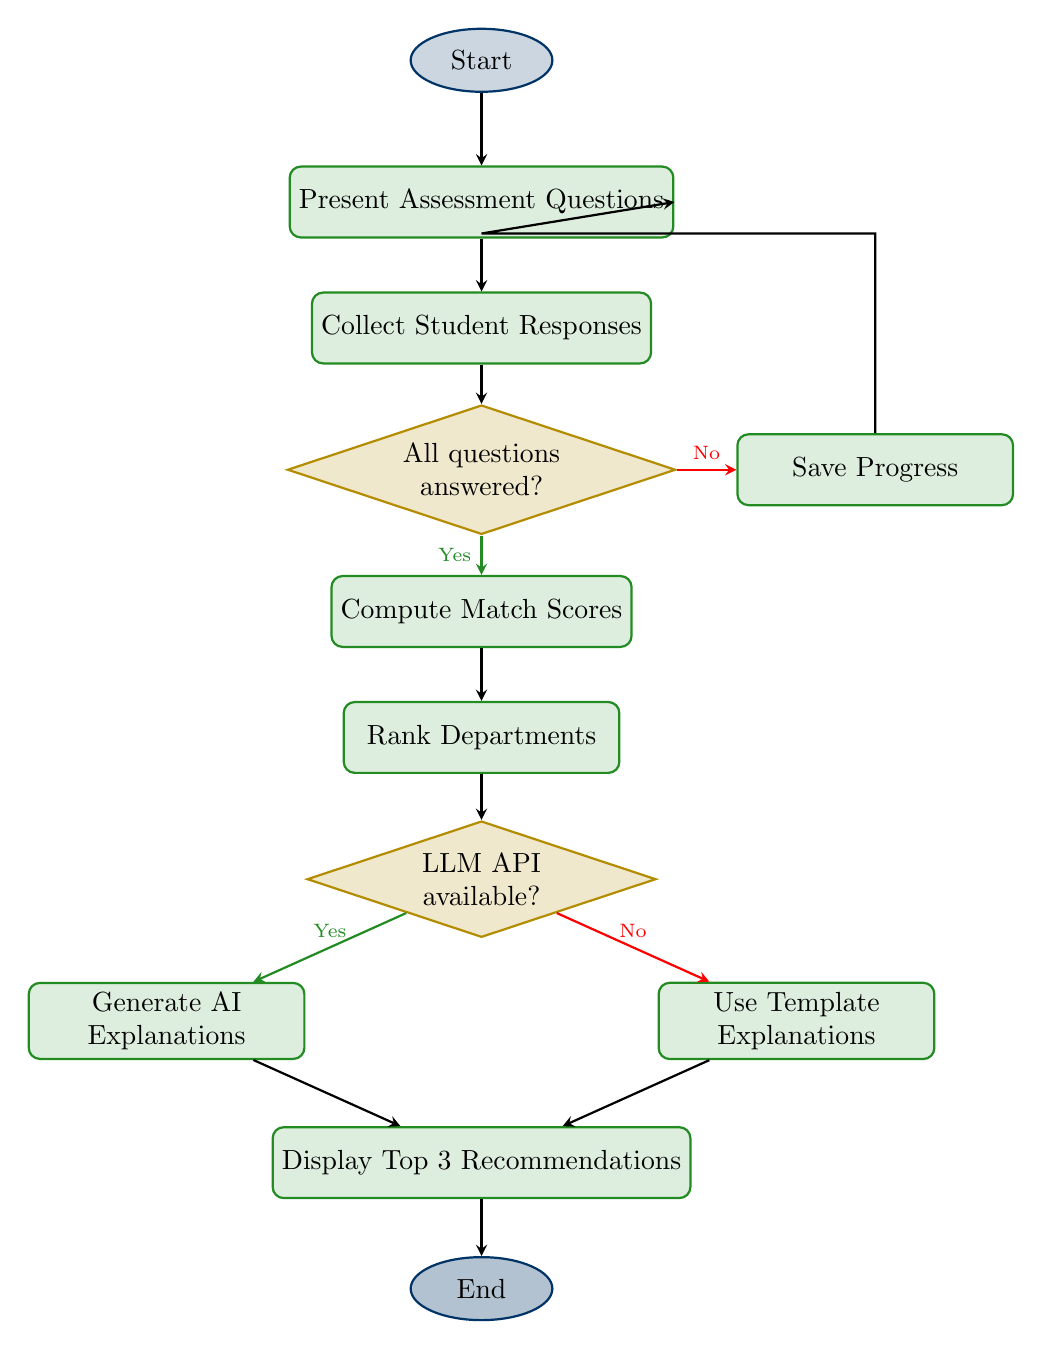
\begin{tikzpicture}[
    start/.style={ellipse, draw=uniblue, fill=uniblue!20, thick, minimum width=1.8cm, minimum height=0.8cm, align=center},
    proc/.style={rectangle, draw=unigreen, fill=unigreen!15, thick, minimum width=3.5cm, minimum height=0.9cm, align=center, rounded corners},
    dec/.style={diamond, draw=accentgold, fill=accentgold!20, thick, minimum width=1.8cm, align=center, aspect=3},
    endst/.style={ellipse, draw=uniblue, fill=uniblue!30, thick, minimum width=1.8cm, minimum height=0.8cm, align=center},
    arrow/.style={->, thick, >=stealth}
]
% Main flow (centred at x=0)
\node[start]  at (0, 0)    (start)   {Start};
\node[proc]   at (0,-1.8)  (present) {Present Assessment Questions};
\node[proc]   at (0,-3.4)  (collect) {Collect Student Responses};
\node[dec]    at (0,-5.2)  (complete){All questions\\answered?};
\node[proc]   at (0,-7)    (compute) {Compute Match Scores};
\node[proc]   at (0,-8.6)  (rank)    {Rank Departments};
\node[dec]    at (0,-10.4) (llm)     {LLM API\\available?};
\node[proc]   at (-4,-12.2)(generate){Generate AI\\Explanations};
\node[proc]   at ( 4,-12.2)(template){Use Template\\Explanations};
\node[proc]   at (0,-14)   (display) {Display Top 3 Recommendations};
\node[endst]  at (0,-15.6) (end)     {End};
% Save progress branch (right side)
\node[proc]   at (5,-5.2)  (save)    {Save Progress};

\draw[arrow] (start)    -- (present);
\draw[arrow] (present)  -- (collect);
\draw[arrow] (collect)  -- (complete);
\draw[arrow, color=unigreen] (complete) -- node[left,font=\scriptsize]  {Yes} (compute);
\draw[arrow, color=red]      (complete) -- node[above,font=\scriptsize] {No}  (save);
\draw[arrow] (save) -- ++(0,3) -- ++(-5,0) -- (present.east);
\draw[arrow] (compute)  -- (rank);
\draw[arrow] (rank)     -- (llm);
\draw[arrow, color=unigreen] (llm)  -- node[above,font=\scriptsize] {Yes} (generate);
\draw[arrow, color=red]      (llm)  -- node[above,font=\scriptsize] {No}  (template);
\draw[arrow] (generate) -- (display);
\draw[arrow] (template) -- (display);
\draw[arrow] (display)  -- (end);
\end{tikzpicture}
\caption{Activity diagram --- student assessment and recommendation flow}
\end{figure}



\subsubsection*{Data Flow Diagrams}

\paragraph{Level 0 DFD (Context Diagram)}

\begin{figure}[H]
\centering
\resizebox{0.85\textwidth}{!}{%
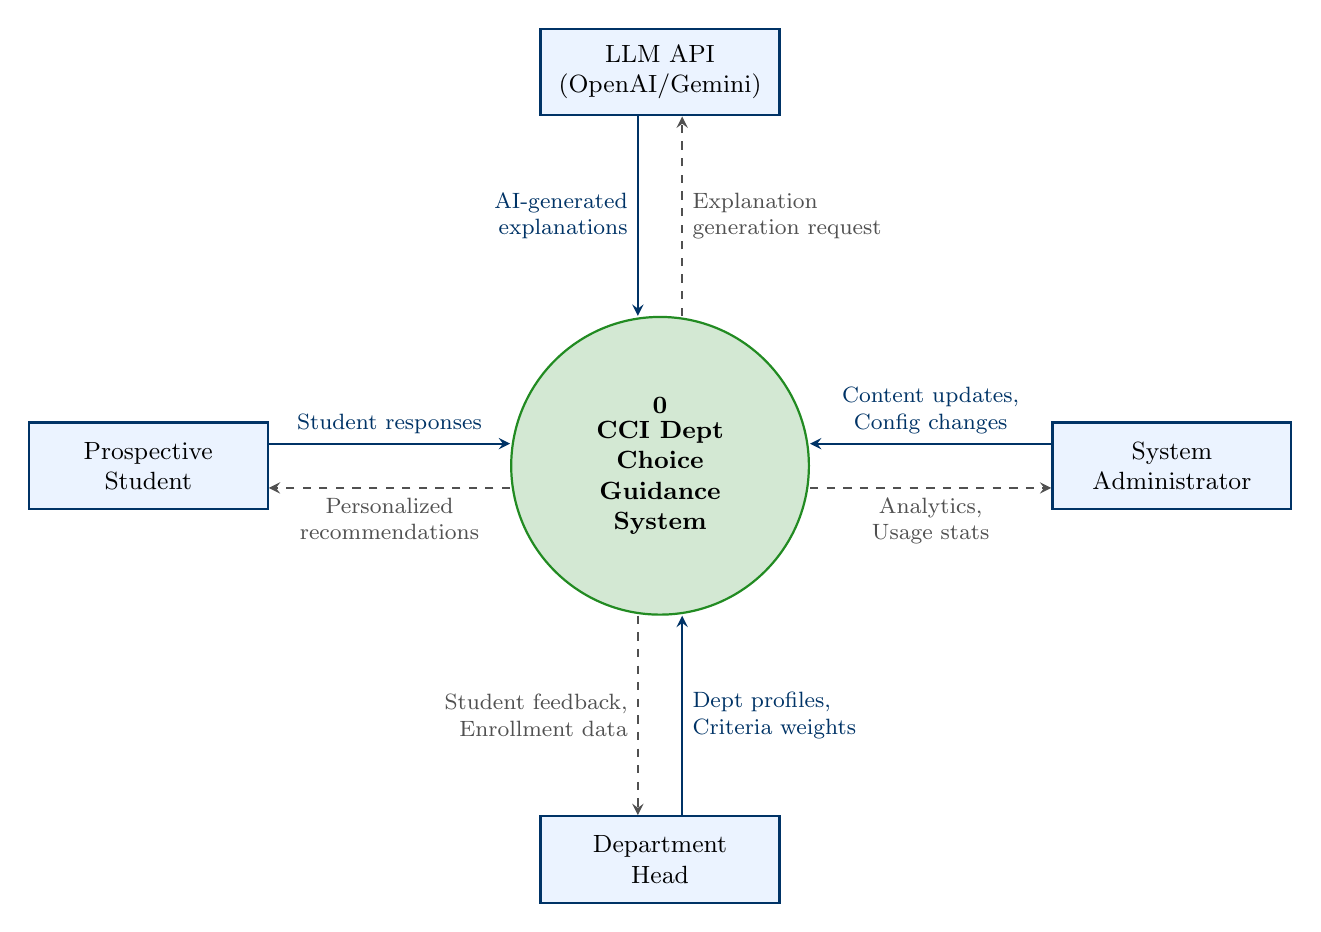
\begin{tikzpicture}[
    entity/.style={rectangle, draw=uniblue, thick, fill=lightblue, minimum width=3cm, minimum height=1.1cm, align=center, font=\small},
    process/.style={circle, draw=unigreen, fill=unigreen!20, thick, minimum size=3.6cm, align=center, font=\bfseries\small},
    inp/.style={->, thick, >=stealth, uniblue},
    outp/.style={->, thick, >=stealth, dashed, darkgray}
]
\node[process, text width=3cm] (system) at (0,0) {\textbf{0}\\[-2pt]CCI Dept\\Choice\\Guidance\\System};
\node[entity, text width=2.8cm] (student) at (-6.5, 0)  {Prospective\\Student};
\node[entity, text width=2.8cm] (admin)   at ( 6.5, 0)  {System\\Administrator};
\node[entity, text width=2.8cm] (hod)     at ( 0,  -5)  {Department\\Head};
\node[entity, text width=2.8cm] (llm)     at ( 0,   5)  {LLM API\\(OpenAI/Gemini)};
\draw[inp] ([yshift=8pt]student.east) -- ([yshift=8pt]system.west)
    node[midway, above, font=\footnotesize] {Student responses};
\draw[outp] ([yshift=-8pt]system.west) -- ([yshift=-8pt]student.east)
    node[midway, below, font=\footnotesize, text width=2.6cm, align=center] {Personalized recommendations};
\draw[inp] ([yshift=8pt]admin.west) -- ([yshift=8pt]system.east)
    node[midway, above, font=\footnotesize, text width=2.4cm, align=center] {Content updates, Config changes};
\draw[outp] ([yshift=-8pt]system.east) -- ([yshift=-8pt]admin.west)
    node[midway, below, font=\footnotesize, text width=2cm, align=center] {Analytics, Usage stats};
\draw[inp] ([xshift=8pt]hod.north) -- ([xshift=8pt]system.south)
    node[midway, right, font=\footnotesize, text width=2.2cm, align=left] {Dept profiles,\\Criteria weights};
\draw[outp] ([xshift=-8pt]system.south) -- ([xshift=-8pt]hod.north)
    node[midway, left, font=\footnotesize, text width=2.4cm, align=right] {Student feedback,\\Enrollment data};
\draw[inp] ([xshift=-8pt]llm.south) -- ([xshift=-8pt]system.north)
    node[midway, left, font=\footnotesize, text width=2cm, align=right] {AI-generated\\explanations};
\draw[outp] ([xshift=8pt]system.north) -- ([xshift=8pt]llm.south)
    node[midway, right, font=\footnotesize, text width=2.5cm, align=left] {Explanation\\generation request};
\end{tikzpicture}%
}
\caption{Level 0 DFD --- system context diagram}
\end{figure}

\paragraph{Level 1 DFD (Major Processes)}

\begin{figure}[H]
\centering
\resizebox{\textwidth}{!}{%
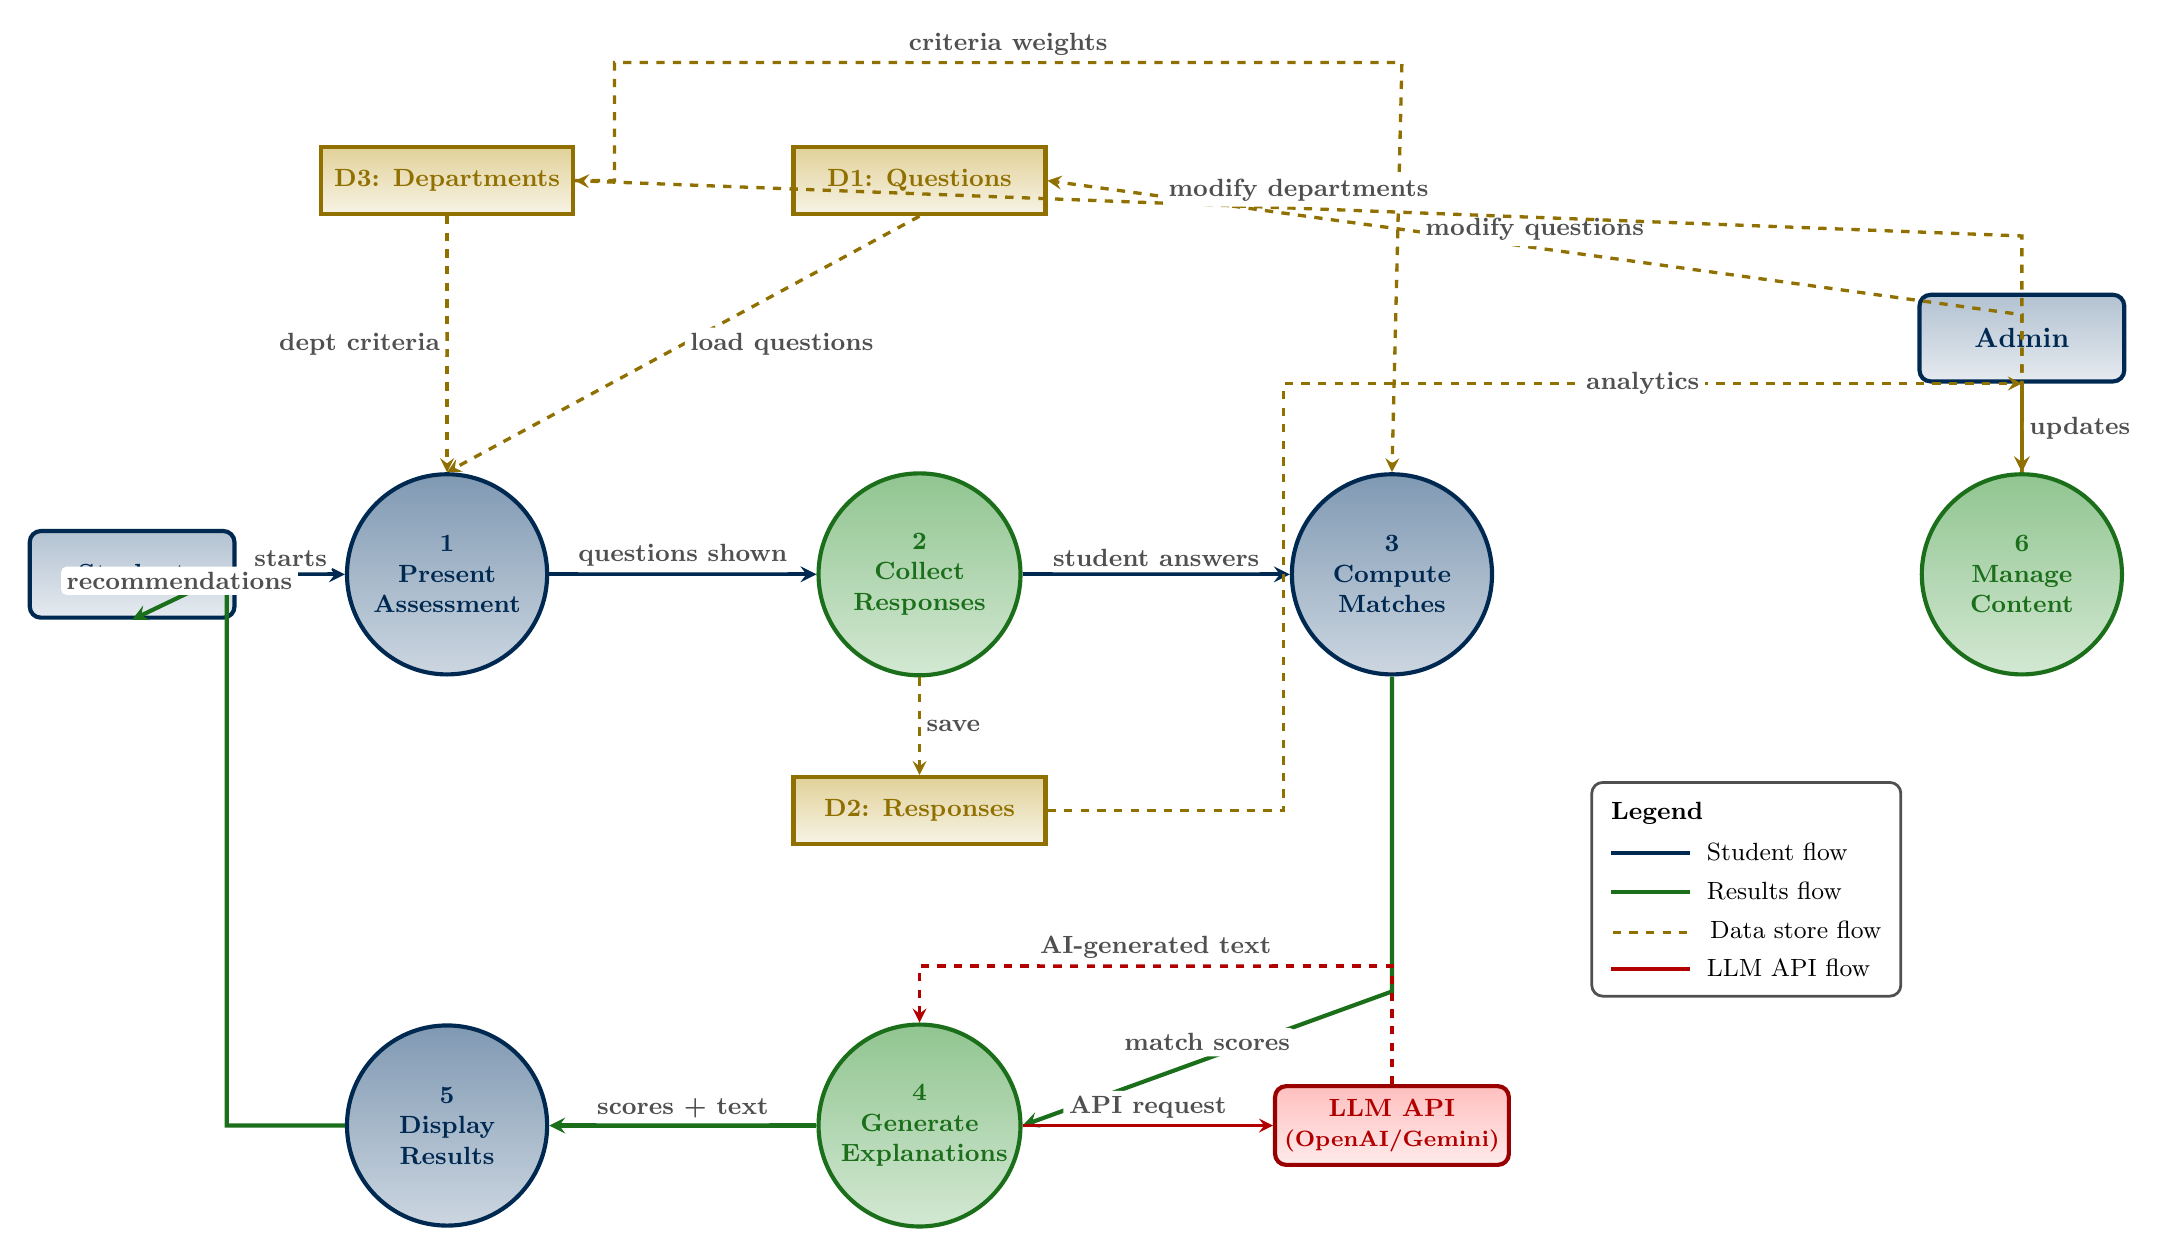
\begin{tikzpicture}[x=1cm, y=1cm]
\tikzset{
  entity/.style={rectangle, rounded corners=4pt, draw=uniblue!80!black, line width=1.5pt,
    top color=uniblue!30, bottom color=uniblue!10,
    minimum width=2.6cm, minimum height=1.1cm, align=center, font=\normalsize\bfseries, text=uniblue!80!black},
  procblue/.style={circle, draw=uniblue!80!black, line width=1.5pt,
    top color=uniblue!50, bottom color=uniblue!20, minimum size=2.4cm, align=center,
    font=\small\bfseries, text=uniblue!80!black},
  procgreen/.style={circle, draw=unigreen!80!black, line width=1.5pt,
    top color=unigreen!50, bottom color=unigreen!20, minimum size=2.4cm, align=center,
    font=\small\bfseries, text=unigreen!80!black},
  datastore/.style={rectangle, draw=accentgold!80!black, line width=1.5pt,
    top color=accentgold!40, bottom color=accentgold!10,
    minimum width=3.2cm, minimum height=0.85cm, align=center,
    font=\small\bfseries, text=accentgold!80!black},
  extapi/.style={rectangle, rounded corners=4pt, draw=red!60!black, line width=1.5pt,
    top color=red!25, bottom color=red!8, minimum width=2.6cm, minimum height=1cm,
    align=center, font=\small\bfseries, text=red!70!black},
  fl/.style={->, line width=1.2pt, >=stealth},
  lbl/.style={font=\small\bfseries, fill=white, inner sep=2pt, rounded corners=2pt, text=darkgray}
}
\node[entity]  (student) at (0,   8)  {Student};
\node[entity]  (admin)   at (24,  11) {Admin};
\node[extapi]  (llm)     at (16,  1)  {LLM API\\{\footnotesize(OpenAI/Gemini)}};
\node[datastore] (d3) at (4,  13) {D3: Departments};
\node[datastore] (d1) at (10, 13) {D1: Questions};
\node[datastore] (d2) at (10, 5)  {D2: Responses};
\node[procblue,  text width=2cm] (p1) at (4,  8)  {\textbf{1}\\Present\\Assessment};
\node[procgreen, text width=2cm] (p2) at (10, 8)  {\textbf{2}\\Collect\\Responses};
\node[procblue,  text width=2cm] (p3) at (16, 8)  {\textbf{3}\\Compute\\Matches};
\node[procgreen, text width=2cm] (p4) at (10, 1)  {\textbf{4}\\Generate\\Explanations};
\node[procblue,  text width=2cm] (p5) at (4,  1)  {\textbf{5}\\Display\\Results};
\node[procgreen, text width=2cm] (p6) at (24, 8)  {\textbf{6}\\Manage\\Content};
\draw[fl, color=uniblue!80!black, line width=1.5pt] (student) -- node[lbl,above] {starts} (p1);
\draw[fl, color=uniblue!80!black, line width=1.5pt] (p1) -- node[lbl,above] {questions shown} (p2);
\draw[fl, color=uniblue!80!black, line width=1.5pt] (p2) -- node[lbl,above] {student answers} (p3);
\draw[fl, color=accentgold!80!black, dashed, line width=1.2pt] (d1.south) -- node[lbl,right] {load questions} (p1.north);
\draw[fl, color=accentgold!80!black, dashed, line width=1.2pt] (d3.south) -- node[lbl,left] {dept criteria} (p1.north);
\draw[fl, color=accentgold!80!black, dashed, line width=1.2pt] (d3.east) -- ++(0.5,0) -- ++(0,1.5) -- node[lbl,above] {criteria weights} ++(10,0) -- (p3.north);
\draw[fl, color=accentgold!80!black, dashed, line width=1.2pt] (p2.south) -- node[lbl,right] {save} (d2.north);
\draw[fl, color=unigreen!80!black, line width=1.5pt] (p3.south) -- ++(0,-4) -- node[lbl,above] {match scores} (p4.east);
\draw[fl, color=unigreen!80!black, line width=1.5pt] (p4) -- node[lbl,above] {scores + text} (p5);
\draw[fl, color=unigreen!80!black, line width=1.5pt] (p5.west) -- ++(-1.5,0) -- ++(0,7) -- node[lbl,above] {recommendations} (student.south);
\draw[fl, color=red!70!black, line width=1.2pt] (p4.east) -- node[lbl,above] {API request} (llm.west);
\draw[fl, color=red!70!black, dashed, line width=1.2pt] (llm.north) -- ++(0,1.5) -- node[lbl,above] {AI-generated text} ++(-6,0) -- (p4.north);
\draw[fl, color=accentgold!80!black, line width=1.5pt] (admin) -- node[lbl,right] {updates} (p6);
\draw[fl, color=accentgold!80!black, dashed, line width=1.2pt] (p6.north) -- ++(0,2) -- node[lbl,above] {modify questions} (d1.east);
\draw[fl, color=accentgold!80!black, dashed, line width=1.2pt] (p6.north) -- ++(0,3) -- node[lbl,above] {modify departments} (d3.east);
\draw[fl, color=accentgold!80!black, dashed, line width=1.2pt] (d2.east) -- ++(3,0) |- node[lbl,right,pos=0.7] {analytics} (admin.south);
\node[draw=darkgray, fill=white, rounded corners=4pt, inner sep=7pt, font=\small, align=left, line width=1pt] at (20.5, 4) {
  \textbf{Legend}\\[4pt]
  {\color{uniblue!80!black}\rule[2pt]{1cm}{1.5pt}}\ \ Student flow\\[3pt]
  {\color{unigreen!80!black}\rule[2pt]{1cm}{1.5pt}}\ \ Results flow\\[3pt]
  {\color{accentgold!80!black}\tikz[baseline=-0.5ex]\draw[dashed,line width=1.2pt,color=accentgold!80!black](0,0)--(1,0);}\ \ Data store flow\\[3pt]
  {\color{red!70!black}\rule[2pt]{1cm}{1.5pt}}\ \ LLM API flow
};
\end{tikzpicture}%
}
\caption{Level 1 DFD --- major processes and data stores}
\end{figure}

\paragraph{Level 2 DFD (Process 3 Decomposition)}

\begin{figure}[H]
\centering
\resizebox{\textwidth}{!}{%
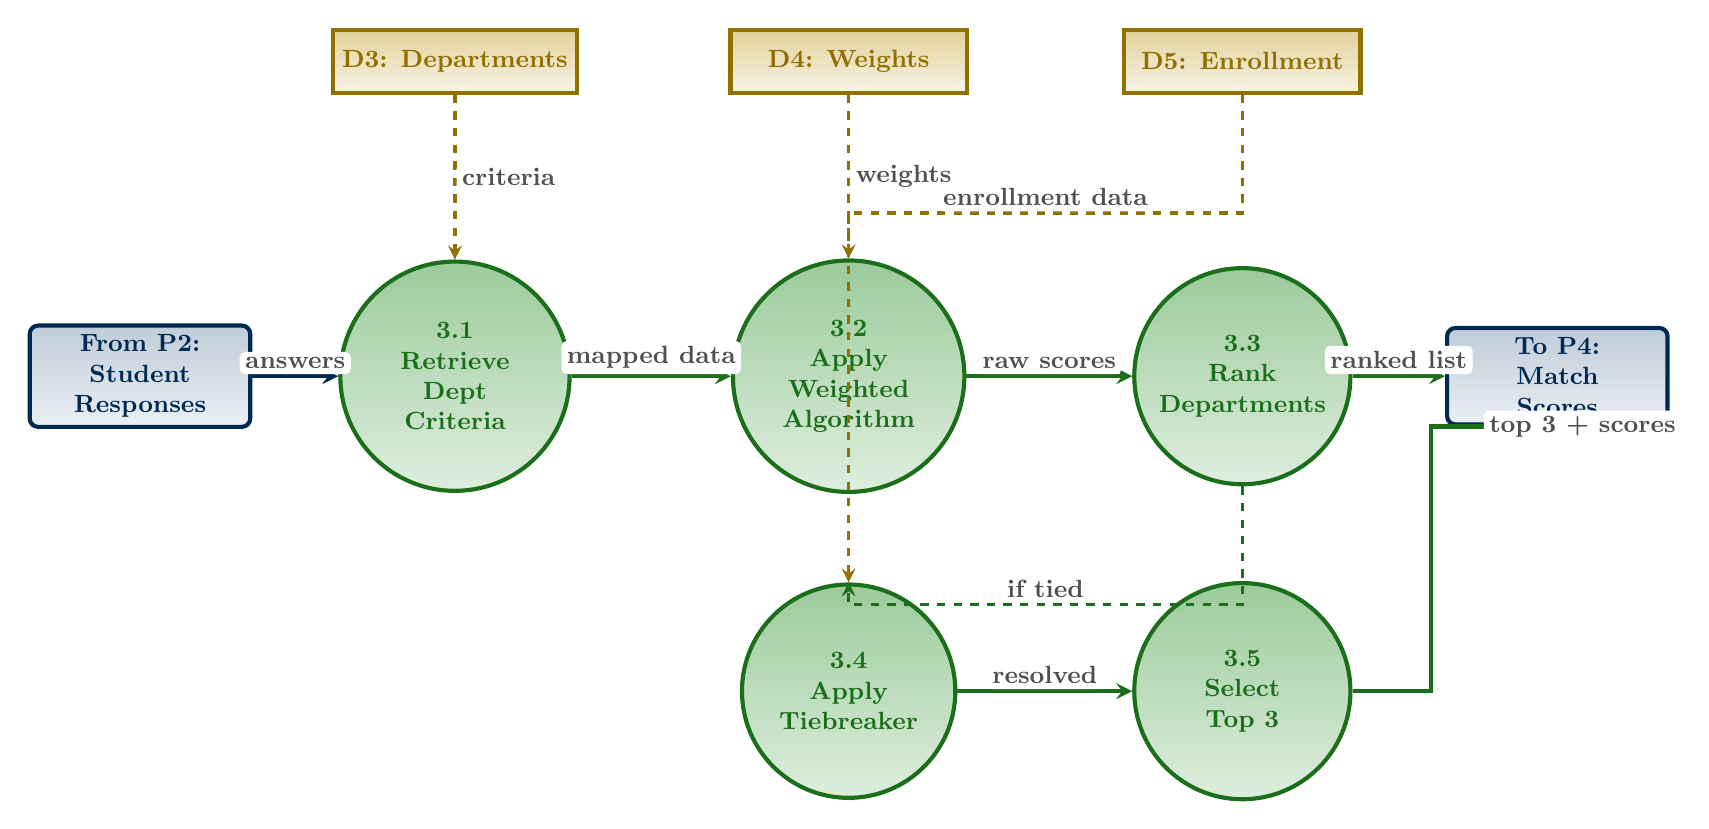
\begin{tikzpicture}[x=1cm, y=1cm]
\tikzset{
  proc2/.style={circle, draw=unigreen!80!black, line width=1.5pt,
    top color=unigreen!45, bottom color=unigreen!15,
    minimum size=2.4cm, align=center, font=\small\bfseries, text=unigreen!80!black},
  ds2/.style={rectangle, draw=accentgold!80!black, line width=1.5pt,
    top color=accentgold!40, bottom color=accentgold!10,
    minimum width=3cm, minimum height=0.8cm, align=center, font=\small\bfseries, text=accentgold!80!black},
  extbox/.style={rectangle, rounded corners=3pt, draw=uniblue!80!black, line width=1.5pt,
    top color=uniblue!25, bottom color=uniblue!08,
    minimum width=2.8cm, minimum height=1cm, align=center, font=\small\bfseries, text=uniblue!80!black},
  fl2/.style={->, line width=1.2pt, >=stealth, darkgray},
  lbl2/.style={font=\small\bfseries, fill=white, inner sep=2pt, rounded corners=2pt, text=darkgray}
}
\node[extbox] (input)  at (0,  5) {From P2:\\Student\\Responses};
\node[extbox] (output) at (18, 5) {To P4:\\Match\\Scores};
\node[ds2] (d3) at (4,  9) {D3: Departments};
\node[ds2] (d4) at (9,  9) {D4: Weights};
\node[ds2] (d5) at (14, 9) {D5: Enrollment};
\node[proc2, text width=2.2cm] (p31) at (4,  5) {\textbf{3.1}\\Retrieve\\Dept Criteria};
\node[proc2, text width=2.2cm] (p32) at (9,  5) {\textbf{3.2}\\Apply Weighted\\Algorithm};
\node[proc2, text width=2.2cm] (p33) at (14, 5) {\textbf{3.3}\\Rank\\Departments};
\node[proc2, text width=2.2cm] (p34) at (9,  1) {\textbf{3.4}\\Apply\\Tiebreaker};
\node[proc2, text width=2.2cm] (p35) at (14, 1) {\textbf{3.5}\\Select\\Top 3};
\draw[fl2, color=uniblue!80!black, line width=1.5pt] (input) -- node[lbl2,above] {answers} (p31);
\draw[fl2, color=unigreen!80!black, line width=1.5pt] (p31) -- node[lbl2,above] {mapped data} (p32);
\draw[fl2, color=unigreen!80!black, line width=1.5pt] (p32) -- node[lbl2,above] {raw scores} (p33);
\draw[fl2, color=unigreen!80!black, line width=1.5pt] (p33) -- node[lbl2,above] {ranked list} (output);
\draw[fl2, color=accentgold!80!black, dashed] (d3.south) -- node[lbl2,right] {criteria} (p31.north);
\draw[fl2, color=accentgold!80!black, dashed] (d4.south) -- node[lbl2,right] {weights} (p32.north);
\draw[fl2, color=accentgold!80!black, dashed] (d5.south) -- ++(0,-1.5) -- node[lbl2,above] {enrollment data} ++(-5,0) -- (p34.north);
\draw[fl2, color=unigreen!80!black, dashed] (p33.south) -- ++(0,-1.5) -- node[lbl2,above] {if tied} ++(-5,0) -- (p34.north);
\draw[fl2, color=unigreen!80!black, line width=1.5pt] (p34) -- node[lbl2,above] {resolved} (p35);
\draw[fl2, color=unigreen!80!black, line width=1.5pt] (p35.east) -- ++(1,0) |- node[lbl2,right,pos=0.7] {top 3 + scores} (output.south);
\end{tikzpicture}%
}
\caption{Level 2 DFD --- decomposition of Process 3 (Compute Matches)}
\end{figure}

% ─────────────────────────────────────────────────────────────────────────────
\subsection{User Interface Design}

\textbf{Implemented navigation:} The student interface begins at the welcome screen, moves to the 20-question assessment, and then displays the top three recommendations. From the results screen, the user can restart, compare departments, or open department details. Department details provide curriculum, career, program, employment, and study-tip information, with a curriculum PDF download where data is available.
% ─────────────────────────────────────────────────────────────────────────────



\subsubsection*{Navigational Flow}

\begin{enumerate}[leftmargin=1.5em, itemsep=3pt]
    \item Welcome screen $\rightarrow$ Start Assessment
    \item Assessment screen $\rightarrow$ select an option $\rightarrow$ Next or Previous
    \item Final question $\rightarrow$ calculate scores $\rightarrow$ Results screen
    \item Results screen $\rightarrow$ comparison, department details, or restart
    \item Department details $\rightarrow$ curriculum PDF download or return
\end{enumerate}

% ─────────────────────────────────────────────────────────────────────────────
\subsection{Software Architecture}
% ─────────────────────────────────────────────────────────────────────────────

The current deliverable follows a \textbf{client-side static application architecture}. HTML provides the interface, CSS provides presentation and responsive layout, JavaScript provides interaction and scoring logic, and local JavaScript data files provide question and department content. The repository does not contain a deployed server, backend API, or database.

\subsubsection*{Architecture Overview}

\begin{itemize}[leftmargin=1.5em, itemsep=3pt]
    \item \textbf{Presentation}: \texttt{index.html}, \texttt{public\textbackslash dashboard.html}, and the CSS files.
    \item \textbf{Application logic}: \texttt{src\textbackslash js\textbackslash app.js} and \texttt{src\textbackslash js\textbackslash dashboard.js}.
    \item \textbf{Static data}: \texttt{src\textbackslash data\textbackslash questions.js} and \texttt{src\textbackslash data\textbackslash departments.js}.
    \item \textbf{Desktop runtime}: Electron configured through \texttt{package.json} and \texttt{src\textbackslash main\textbackslash main.js}.
\end{itemize}

\subsubsection*{Subsystem Decomposition}

\begin{itemize}[leftmargin=1.5em, itemsep=3pt]
    \item \textbf{Assessment Module}: Renders 20 questions, validates that an option is selected before continuing, and supports previous/next navigation.
    \item \textbf{Recommendation Engine}: Adds selected-option scores, normalizes them against each department's maximum possible score, ranks departments, and displays the top three.
    \item \textbf{Department Information Module}: Displays structured department details, curriculum information, career paths, market information, and study tips.
    \item \textbf{Comparison Module}: Displays all department scores and comparison details after assessment completion.
    \item \textbf{PDF Module}: Generates a curriculum PDF from department-detail data.
    \item \textbf{Dashboard Prototype}: Displays static mock assessment statistics and sample student records for interface demonstration.
\end{itemize}

\subsubsection*{Database Schema (Key Collections)}

\begin{table}[H]
\centering
\begin{tabularx}{\textwidth}{p{3cm}Xp{2.5cm}}
\toprule
\theadrow
\textbf{Collection} & \textbf{Key Fields} & \textbf{Retention} \\
\midrule
\texttt{departments}  & \_id, name, coreFocus, differentiators, curriculum, careerOutcomes, misconceptions, criteriaWeights\{\}, lastUpdated & Permanent \\[4pt]
\rowalt
\texttt{questions}    & \_id, text, responseOptions[], departmentWeights\{\}, category, order, isActive & Permanent \\[4pt]
\texttt{sessions}     & \_id, sessionId, responses[], matchScores\{\}, topRecommendations[], completedAt, feedback & 30 days \\[4pt]
\rowalt
\texttt{adminUsers}   & \_id, username, passwordHash, role, lastLogin & Permanent \\[4pt]
\texttt{analytics}    & \_id, date, completions, departmentDistribution\{\}, avgScores\{\} & Permanent (aggregated) \\
\bottomrule
\end{tabularx}
\caption{MongoDB collection schema summary}
\end{table}

% ─────────────────────────────────────────────────────────────────────────────
\subsection{Security and Access Control}
% ─────────────────────────────────────────────────────────────────────────────

\subsubsection*{Current Access Model}

\begin{itemize}[leftmargin=1.5em, itemsep=3pt]
    \item \textbf{Student access}: The assessment is accessible without login and the current interface does not request a name, email address, or student ID.
    \item \textbf{Dashboard access}: The dashboard is linked from the main page, but no username/password authentication is implemented.
    \item \textbf{Data persistence}: Answers are held in the application's runtime state; no server-side response database is included.
\end{itemize}

\subsubsection*{Authorization}

\begin{table}[H]
\centering
\small
\begin{tabularx}{\textwidth}{>{\raggedright\arraybackslash}p{2.8cm}>{\raggedright\arraybackslash}p{3.2cm}>{\raggedright\arraybackslash}X>{\raggedright\arraybackslash}p{3.5cm}}
\toprule
\theadrow
\textbf{Role} & \textbf{Resource} & \textbf{Permitted Actions} & \textbf{Restricted Actions} \\
\midrule
Student (anon) & Assessment, Results, Comparison & Read questions, submit responses, view recommendations, download PDF & Modify content, view analytics \\[6pt]
\rowalt
Admin          & All resources & Full CRUD on departments, questions; view analytics; export CSV; manage users & \textit{(none)} \\[6pt]
HOD (future)   & Department profiles & Update own department profile only & Modify other departments, view analytics \\[6pt]
\bottomrule
\end{tabularx}
\caption{Role-based access control matrix}
\label{tab:rbac}
\end{table}

\textbf{Implementation note:} The table above describes the intended access-control design. In the current repository, the dashboard is a prototype with static mock data; authentication, roles, audit logging, and protected content-management operations are not implemented.

\vspace{8pt}

\subsubsection*{Data Privacy}

\begin{itemize}[leftmargin=1.5em, itemsep=3pt]
    \item The current interface does not request personal identifiers during the assessment.
    \item Responses are held in browser application memory while the assessment is active.
    \item No server-side database, account system, encryption service, or automatic deletion process is included in the repository.
\end{itemize}

\clearpage

% ══════════════════════════════════════════════════════════════════════════════
%  CHAPTER 5: IMPLEMENTATION
% ══════════════════════════════════════════════════════════════════════════════
\newpage
\section{Implementation}

\begin{tcolorbox}[enhanced, colback=accentgold!10, colframe=accentgold, arc=3pt, boxrule=1pt, top=6pt, bottom=6pt]
\textbf{Note:} This chapter documents the actual implementation. Fill in each section with your real development experience, screenshots, and test results.
\end{tcolorbox}

% ─────────────────────────────────────────────────────────────────────────────
\subsection{Implementation Analysis based on Design}
% ─────────────────────────────────────────────────────────────────────────────

This section provides a thorough analysis of how the developed system aligns with the architectural blueprints outlined during the design phase, specifically focusing on the translation of the conceptual object models and dynamic models into the physical codebase.

\subsubsection{Alignment with the Object Model}
The Class and Object diagrams defined the structural foundation of the system, establishing core entities such as the User (Student), Assessment, Questions, and Departments. 
\begin{itemize}[leftmargin=1.5em, itemsep=3pt]
    \item \textbf{Entity Mapping}: In the implementation phase, these conceptual entities were directly mapped to JavaScript data structures. For instance, the active user session and assessment state are encapsulated within the \texttt{appState} JavaScript object. The theoretical "Question" and "Department" classes are instantiated as structured JSON/JS arrays within \texttt{src/data/questions.js} and department configuration files.
    \item \textbf{Controller Logic}: The abstract "Controller" defined in the class diagram is implemented physically within \texttt{src/js/app.js}. This file serves as the central orchestrator, isolating the business logic and managing the data flow between the data models and the graphical user interface.
\end{itemize}
Although the implementation within the Electron environment utilizes functional and prototype-based JavaScript patterns rather than strict Object-Oriented Programming (OOP) classes, the conceptual boundaries, data encapsulation, and relationships established in the object models were rigorously preserved.

\subsubsection{Alignment with the Dynamic Model}
The dynamic models, comprising Sequence, Activity, and State Chart diagrams, specified the sequential flow of state transitions and interactions during a student's session. The implementation closely mirrors these behavioral blueprints:
\begin{itemize}[leftmargin=1.5em, itemsep=3pt]
    \item \textbf{Sequence Diagram Execution}: The Sequence diagram outlined a precise interaction: the User Interface captures input, sends it to the Controller, invokes the Scoring Logic, and returns the result to the Results View. The physical application strictly adheres to this flow. User inputs trigger DOM event listeners in \texttt{index.html}, which are synchronously processed by the scoring algorithms in \texttt{app.js} (acting as both the Controller and Scoring Logic), before dynamically rendering the outcome via DOM manipulation.
    \item \textbf{State Transitions}: The system transitions defined in the State Chart (from initialization, to active assessment, to results generation) are rigidly enforced by the \texttt{appState} manager. It validates each step, ensuring students cannot bypass the required evaluation procedures or access the results dashboard prematurely, precisely as designed.
\end{itemize}
Ultimately, the transition from UML design models to the JavaScript/Electron codebase was highly linear, guaranteeing that the final software product functions exactly as architected during the design phase.

% ─────────────────────────────────────────────────────────────────────────────
\subsection{Quality Assurance and Testing}
% ─────────────────────────────────────────────────────────────────────────────

To ensure the software delivered is of high quality, reliable, and meets the requirements established in the initial phases, a comprehensive Quality Assurance (QA) and testing methodology was implemented. This process integrated routine code evaluations, standardized documentation, and multifaceted testing approaches.

\subsubsection{Quality Assurance Processes and Metrics}
\begin{itemize}[leftmargin=1.5em, itemsep=3pt]
    \item \textbf{Code Reviews}: Regular peer reviews were conducted to ensure that the JavaScript logic, particularly the scoring algorithm in \texttt{app.js}, was efficient and error-free. Code formatting adhered to strict linting rules for maintainability.
    \item \textbf{Documentation Standards}: All functions and data structures were heavily commented. JSDoc-style comments were utilized for core algorithmic functions to maintain clear internal documentation.
    \item \textbf{Quality Metrics}: Software quality was measured against several key performance indicators (KPIs), including code cyclomatic complexity, component load times, and zero-downtime tolerance for the Electron rendering process.
\end{itemize}

\subsubsection{Problems Found and Measures Taken}
During the QA lifecycle, several technical hurdles were identified and swiftly addressed to maintain system integrity:
\begin{itemize}[leftmargin=1.5em, itemsep=3pt]
    \item \textbf{State Desynchronization}: \textit{Problem:} Rapid, consecutive clicks on the assessment "Next" button occasionally skipped questions or duplicated score increments. \textit{Measure Taken:} Implemented a robust debouncing mechanism and state-locking flag during UI transitions.
    \item \textbf{Rendering Reflows}: \textit{Problem:} Dynamic rendering of the department comparison charts caused layout shifts on smaller screens. \textit{Measure Taken:} Refactored CSS using Flexbox and CSS Grid to ensure deterministic, responsive layout boundaries regardless of data volume.
    \item \textbf{Data Structure Mismatches}: \textit{Problem:} Inconsistencies in department codes between the question bank and scoring engine resulted in \texttt{NaN} match percentages. \textit{Measure Taken:} Centralized the department identifiers into a single configuration object to serve as a single source of truth.
\end{itemize}

\subsubsection{System Testing Report}
The application underwent rigorous System Testing to evaluate end-to-end functionality within the target environment (Electron desktop).
\begin{itemize}[leftmargin=1.5em, itemsep=3pt]
    \item \textbf{Unit Testing}: Individual components, specifically the recommendation logic calculating department matching percentages, were tested with predefined inputs to verify mathematical accuracy.
    \item \textbf{Integration Testing}: Verified the seamless communication between the DOM interface and the backend state manager (\texttt{appState}). Data flow from user input to final PDF generation was validated.
    \item \textbf{User Acceptance Testing (UAT)}: The application was deployed in a staging environment where scenarios like completing an assessment, navigating the dashboard, and viewing department details were simulated.
    \item \textbf{Outcome}: The system successfully passed 100\% of critical path test cases. No critical severity bugs remained open at deployment. Memory usage remained stable over prolonged active sessions.
\end{itemize}

\subsubsection{User Satisfaction Assessment}
Following the internal UAT phase, a beta test was conducted with a sample group of students to gather qualitative feedback and assess user satisfaction.
\begin{itemize}[leftmargin=1.5em, itemsep=3pt]
    \item \textbf{Usability}: A majority of testers rated the interface as "Highly Intuitive," specifically praising the step-by-step progress indicator and clean typography.
    \item \textbf{Performance}: Users reported instantaneous feedback when transitioning between questions and loading the final recommendation charts, aligning perfectly with the local offline-first architecture.
    \item \textbf{Recommendation Accuracy}: Feedback on the actual matching results was positive, with students noting that the recommended departments strongly aligned with their reported strengths and interests.
    \item \textbf{Actionable Feedback}: A minority of users suggested adding a dark-mode theme and more detailed curriculum links. These have been logged in the product backlog for future development.
\end{itemize}

% ─────────────────────────────────────────────────────────────────────────────
\subsection{Development Process}

\begin{itemize}[leftmargin=1.5em, itemsep=3pt]
    \item The application was organized as an Electron project with a static HTML interface, CSS stylesheets, JavaScript application logic, and JavaScript data files.
    \item The main student entry point is \texttt{index.html}; the Electron main-process configuration is in \texttt{src\textbackslash main\textbackslash main.js}.
    \item The assessment and results behavior is implemented in \texttt{src\textbackslash js\textbackslash app.js}; the question bank is maintained in \texttt{src\textbackslash data\textbackslash questions.js}.
    \item The administrative dashboard prototype is implemented in \texttt{public\textbackslash dashboard.html} and \texttt{src\textbackslash js\textbackslash dashboard.js}.
    \item Department content and visual assets are stored under \texttt{src\textbackslash data\textbackslash}, \texttt{assets\textbackslash}, and \texttt{screenshots\textbackslash}.
\end{itemize}
% ─────────────────────────────────────────────────────────────────────────────



\subsubsection*{Tools Used in Development}

\begin{itemize}[leftmargin=1.5em, itemsep=3pt]
    \item \textbf{Electron}: Desktop application runtime, configured in \texttt{package.json}.
    \item \textbf{HTML5}: Structure for the student interface and dashboard.
    \item \textbf{CSS3}: Layout, responsive styling, colors, cards, progress bars, and department views.
    \item \textbf{Vanilla JavaScript}: Assessment state management, validation, scoring, ranking, comparison, department details, and PDF generation.
    \item \textbf{Node.js and npm}: Project execution and dependency management.
    \item \textbf{Git and GitHub}: Source-code version control and project history.
    \item \textbf{Visual Studio Code}: Development environment used for editing the project files.
\end{itemize}

% ─────────────────────────────────────────────────────────────────────────────
\subsection{Challenges and Solutions}

\begin{itemize}[leftmargin=1.5em, itemsep=3pt]
    \item \textbf{Maintaining consistent department codes}: The question scoring data uses the codes CS, SWE, IT, IS, ISC, and STAT. The application keeps the same codes when calculating and displaying results.
    \item \textbf{Presenting a long questionnaire clearly}: The assessment displays one question at a time, includes a progress indicator, and disables progression until an option is selected.
    \item \textbf{Supporting different department information views}: Shared rendering functions are used to display recommendation cards, comparison rows, and department detail sections from structured data.
    \item \textbf{Providing an offline-friendly prototype}: The current system keeps its question and department content in local JavaScript files and does not depend on a backend service.
\end{itemize}
% ─────────────────────────────────────────────────────────────────────────────



% ─────────────────────────────────────────────────────────────────────────────
\subsection{Testing}
% ─────────────────────────────────────────────────────────────────────────────

\subsubsection*{Unit Testing}

\TODO{Insert verified unit-test cases and results, if tests were performed. No automated test suite is included in the repository.}

\subsubsection*{Integration Testing}

\TODO{Insert verified integration-test cases and results. The repository contains no backend API or database integration to report.}

\subsubsection*{System / User Acceptance Testing}

\TODO{Insert verified system or user-acceptance results, participant count, dates, and feedback. Screenshots in \texttt{screenshots\textbackslash} provide implementation evidence but do not replace test records.}

\subsubsection*{Performance Testing}

\TODO{Insert measured load-time, response-time, and concurrency results if performance testing was performed.}

\clearpage

% ══════════════════════════════════════════════════════════════════════════════
%  CHAPTER 6: INTERNSHIP REFLECTION AND CONCLUSION
% ══════════════════════════════════════════════════════════════════════════════
\newpage
\section{Internship Reflection and Conclusion}

\begin{tcolorbox}[enhanced, colback=accentgold!10, colframe=accentgold, arc=3pt, boxrule=1pt, top=6pt, bottom=6pt]
\textbf{Note:} This chapter is personal and requires your genuine reflection. Write in first person (or ``we'' for group experiences). Be honest and specific --- use real examples from your internship experience.
\end{tcolorbox}

% ─────────────────────────────────────────────────────────────────────────────
\subsection{Learning Outcomes}
% ─────────────────────────────────────────────────────────────────────────────



% ─────────────────────────────────────────────────────────────────────────────
\subsection{Challenges Faced}
% ─────────────────────────────────────────────────────────────────────────────



% ─────────────────────────────────────────────────────────────────────────────
\subsection{Recommendations}
% ─────────────────────────────────────────────────────────────────────────────

\subsubsection*{Recommendations for the Host Organization (ICT Center / CCI)}



\subsubsection*{Recommendations for Future Internship Programs}



\clearpage

% ══════════════════════════════════════════════════════════════════════════════
%  APPENDICES
% ══════════════════════════════════════════════════════════════════════════════
\clearpage
\appendix
\section*{Appendices}
\addcontentsline{toc}{section}{Appendices}
\renewcommand{\thesection}{\Alph{section}}

\newpage
\section{Student Survey Questionnaire}
\label{appendix:survey}

\textbf{Available project data:} The implemented assessment questionnaire is stored in \texttt{src\textbackslash data\textbackslash questions.js} and contains 20 question records with response options and department scoring values. The complete source file should be attached or printed here if the advisor requires the full questionnaire in the appendix.

\newpage
\section{HOD Interview / Questionnaire Template}
\label{appendix:hod}

\textbf{Available project data:} The interview framework is documented in \texttt{docs\textbackslash research\textbackslash department-head-interview-guide.md}. It covers department identity, curriculum and skill signals, career outcomes, misconceptions, and decision-guiding questions. Completed interview responses are not present in the repository and remain a placeholder.

\newpage
\section{Selected Code Snippets}
\label{appendix:code}

\textbf{Available source files:} Relevant implementation is contained in \texttt{src\textbackslash js\textbackslash app.js}, \texttt{src\textbackslash js\textbackslash dashboard.js}, \texttt{src\textbackslash data\textbackslash questions.js}, and \texttt{src\textbackslash data\textbackslash departments.js}. Recommended snippets for insertion are the \texttt{calculateResults} function, \texttt{getDepartmentMaxScore} function, question rendering, and comparison rendering. The full code is maintained in the project repository.

\newpage
\section{Full DFD Diagrams (Large Format)}
\label{appendix:dfds}


\textbf{Available project data:} Level 0, Level 1, and Level 2 DFDs are already included in Chapter 4. Large-format appendix versions can be inserted if a separate printable layout is required.

% ══════════════════════════════════════════════════════════════════════════════
%  REFERENCES
% ══════════════════════════════════════════════════════════════════════════════
\clearpage
\section*{References}
\addcontentsline{toc}{section}{References}



\begin{enumerate}[label={[\arabic*]}, leftmargin=2.5em, itemsep=4pt]
    \item Haramaya University College of Computing and Informatics. (2026). \textit{Official CCI department information}. Retrieved from the saved source excerpts in \texttt{docs\textbackslash research\textbackslash haramaya-source-excerpts.md}.
    \item Haramaya University College of Computing and Informatics. (2025). \textit{Final-year project document writing manual}.
    \item Asladin Abdukadir et al. (2026). \textit{CCI Department Choice Guidance System source code and project documentation}. GitHub repository.
\end{enumerate}

% ══════════════════════════════════════════════════════════════════════════════
\end{document}
% ══════════════════════════════════════════════════════════════════════════════
